\documentclass[11pt,final]{article}

\pdfoutput=1 
\newcommand{\rl}[1]{\textcolor{purple}{RL:#1}}
\newcommand{\ia}[1]{\textcolor{orange}{ia:#1}}
\usepackage[utf8]{inputenc}
\usepackage{lmodern} \normalfont %
\usepackage{anyfontsize}
\usepackage[T1]{fontenc}
\DeclareFontShape{T1}{lmr}{bx}{sc} { <-> ssub * cmr/bx/sc }{}
\DeclareFontShape{T1}{lmr}{m}{scit}{ <-> ssub * cmr/m/sc }{}
\DeclareFontShape{T1}{lmr}{bx}{scit}{ <-> ssub * cmr/bx/sc }{}

%
\usepackage{amsthm}
\usepackage{amsmath}
\usepackage[utf8]{inputenc} 
\usepackage{amsmath, amssymb,bm, cases, mathtools, thmtools}
\usepackage{verbatim}
\usepackage{graphicx}
\usepackage{multicol}
\usepackage{tabularx}
\usepackage{mathrsfs} 
\usepackage{algorithm}
\usepackage{algorithmicx}
\usepackage[noend]{algpseudocode}
\usepackage{array,booktabs,arydshln,xcolor}
\usepackage[normalem]{ulem}

\usepackage{multirow}

\usepackage[%
            minnames=1,maxnames=99,maxbibnames=99,minalphanames=1,maxalphanames=99,
		%
		style=alphabetic,
		sorting=nyt,
		sortcites=false, %
        %
		doi=false,url=false,
		uniquename=init,
		giveninits=true,
		hyperref,natbib,
		%
		backend=biber]{biblatex}
\renewbibmacro{in:}{%
	\ifentrytype{article}{}{\printtext{\bibstring{in}\intitlepunct}}}

\addbibresource{refs.bib} 


\usepackage{inconsolata}
\usepackage{dsfont}
\usepackage{hyperref}
\usepackage{tikz}
\usepackage{listings} 
\usepackage[shortlabels]{enumitem}
\usepackage{nicefrac}
\usepackage{lineno}
\usepackage{bbm}
\usepackage{subcaption}
\usepackage{datetime}

\DeclareMathAlphabet\EuRoman{U}{eur}{m}{n}
\SetMathAlphabet\EuRoman{bold}{U}{eur}{b}{n}
\newcommand{\eurom}{\EuRoman}


%
\declaretheorem[style=plain,numberwithin=section,name=Theorem]{theorem}
\declaretheorem[style=plain,sibling=theorem,name=Lemma]{lemma}
\declaretheorem[style=plain,sibling=theorem,name=Proposition]{proposition}
\declaretheorem[style=plain,sibling=theorem,name=Corollary]{corollary}

\declaretheorem[style=definition,sibling=theorem,name=Definition]{definition}
\declaretheorem[style=definition,qed=$\triangleleft$,sibling=theorem,name=Example]{example}
\declaretheorem[style=remark,qed=$\triangleleft$,sibling=theorem,name=Remark]{remark}
%

%
\numberwithin{theorem}{section}

\renewcommand{\appendixname}{}
%

\usepackage{xparse}
\usepackage{xstring}
\usepackage{xspace}

\usepackage{xfrac}


%
\setlength\unitlength{1mm}
\newcommand{\twodots}{\mathinner {\ldotp \ldotp}}
% bb font symbols
\newcommand{\Rho}{\mathrm{P}}
\newcommand{\Tau}{\mathrm{T}}

\newfont{\bbb}{msbm10 scaled 700}
\newcommand{\CCC}{\mbox{\bbb C}}

\newfont{\bb}{msbm10 scaled 1100}
\newcommand{\CC}{\mbox{\bb C}}
\newcommand{\PP}{\mbox{\bb P}}
\newcommand{\RR}{\mbox{\bb R}}
\newcommand{\QQ}{\mbox{\bb Q}}
\newcommand{\ZZ}{\mbox{\bb Z}}
\newcommand{\FF}{\mbox{\bb F}}
\newcommand{\GG}{\mbox{\bb G}}
\newcommand{\EE}{\mbox{\bb E}}
\newcommand{\NN}{\mbox{\bb N}}
\newcommand{\KK}{\mbox{\bb K}}
\newcommand{\HH}{\mbox{\bb H}}
\newcommand{\SSS}{\mbox{\bb S}}
\newcommand{\UU}{\mbox{\bb U}}
\newcommand{\VV}{\mbox{\bb V}}


\newcommand{\yy}{\mathbbm{y}}
\newcommand{\xx}{\mathbbm{x}}
\newcommand{\zz}{\mathbbm{z}}
\newcommand{\sss}{\mathbbm{s}}
\newcommand{\rr}{\mathbbm{r}}
\newcommand{\pp}{\mathbbm{p}}
\newcommand{\qq}{\mathbbm{q}}
\newcommand{\ww}{\mathbbm{w}}
\newcommand{\hh}{\mathbbm{h}}
\newcommand{\vvv}{\mathbbm{v}}

% Vectors

\newcommand{\av}{{\bf a}}
\newcommand{\bv}{{\bf b}}
\newcommand{\cv}{{\bf c}}
\newcommand{\dv}{{\bf d}}
\newcommand{\ev}{{\bf e}}
\newcommand{\fv}{{\bf f}}
\newcommand{\gv}{{\bf g}}
\newcommand{\hv}{{\bf h}}
\newcommand{\iv}{{\bf i}}
\newcommand{\jv}{{\bf j}}
\newcommand{\kv}{{\bf k}}
\newcommand{\lv}{{\bf l}}
\newcommand{\mv}{{\bf m}}
\newcommand{\nv}{{\bf n}}
\newcommand{\ov}{{\bf o}}
\newcommand{\pv}{{\bf p}}
\newcommand{\qv}{{\bf q}}
\newcommand{\rv}{{\bf r}}
\newcommand{\sv}{{\bf s}}
\newcommand{\tv}{{\bf t}}
\newcommand{\uv}{{\bf u}}
\newcommand{\wv}{{\bf w}}
\newcommand{\vv}{{\bf v}}
\newcommand{\xv}{{\bf x}}
\newcommand{\yv}{{\bf y}}
\newcommand{\zv}{{\bf z}}
\newcommand{\zerov}{{\bf 0}}
\newcommand{\onev}{{\bf 1}}

% Matrices

\newcommand{\Am}{{\bf A}}
\newcommand{\Bm}{{\bf B}}
\newcommand{\Cm}{{\bf C}}
\newcommand{\Dm}{{\bf D}}
\newcommand{\Em}{{\bf E}}
\newcommand{\Fm}{{\bf F}}
\newcommand{\Gm}{{\bf G}}
\newcommand{\Hm}{{\bf H}}
\newcommand{\Id}{{\bf I}}
\newcommand{\Jm}{{\bf J}}
\newcommand{\Km}{{\bf K}}
\newcommand{\Lm}{{\bf L}}
\newcommand{\Mm}{{\bf M}}
\newcommand{\Nm}{{\bf N}}
\newcommand{\Om}{{\bf O}}
\newcommand{\Pm}{{\bf P}}
\newcommand{\Qm}{{\bf Q}}
\newcommand{\Rm}{{\bf R}}
\newcommand{\Sm}{{\bf S}}
\newcommand{\Tm}{{\bf T}}
\newcommand{\Um}{{\bf U}}
\newcommand{\Wm}{{\bf W}}
\newcommand{\Vm}{{\bf V}}
\newcommand{\Xm}{{\bf X}}
\newcommand{\Ym}{{\bf Y}}
\newcommand{\Zm}{{\bf Z}}

% Calligraphic

\newcommand{\Ac}{{\cal A}}
\newcommand{\Bc}{{\cal B}}
\newcommand{\Cc}{{\cal C}}
\newcommand{\Dc}{{\cal D}}
\newcommand{\Ec}{{\cal E}}
\newcommand{\Fc}{{\cal F}}
\newcommand{\Gc}{{\cal G}}
\newcommand{\Hc}{{\cal H}}
\newcommand{\Ic}{{\cal I}}
\newcommand{\Jc}{{\cal J}}
\newcommand{\Kc}{{\cal K}}
\newcommand{\Lc}{{\cal L}}
\newcommand{\Mc}{{\cal M}}
\newcommand{\Nc}{{\cal N}}
\newcommand{\nc}{{\cal n}}
\newcommand{\Oc}{{\cal O}}
\newcommand{\Pc}{{\cal P}}
\newcommand{\Qc}{{\cal Q}}
\newcommand{\Rc}{{\cal R}}
\newcommand{\Sc}{{\cal S}}
\newcommand{\Tc}{{\cal T}}
\newcommand{\Uc}{{\cal U}}
\newcommand{\Wc}{{\cal W}}
\newcommand{\Vc}{{\cal V}}
\newcommand{\Xc}{{\cal X}}
\newcommand{\Yc}{{\cal Y}}
\newcommand{\Zc}{{\cal Z}}

% Bold greek letters

\newcommand{\alphav}{\hbox{\boldmath$\alpha$}}
\newcommand{\betav}{\hbox{\boldmath$\beta$}}
\newcommand{\gammav}{\hbox{\boldmath$\gamma$}}
\newcommand{\deltav}{\hbox{\boldmath$\delta$}}
\newcommand{\etav}{\hbox{\boldmath$\eta$}}
\newcommand{\lambdav}{\hbox{\boldmath$\lambda$}}
\newcommand{\epsilonv}{\hbox{\boldmath$\epsilon$}}
\newcommand{\nuv}{\hbox{\boldmath$\nu$}}
\newcommand{\muv}{\hbox{\boldmath$\mu$}}
\newcommand{\zetav}{\hbox{\boldmath$\zeta$}}
\newcommand{\phiv}{\hbox{\boldmath$\phi$}}
\newcommand{\psiv}{\hbox{\boldmath$\psi$}}
\newcommand{\thetav}{\hbox{\boldmath$\theta$}}
\newcommand{\tauv}{\hbox{\boldmath$\tau$}}
\newcommand{\omegav}{\hbox{\boldmath$\omega$}}
\newcommand{\xiv}{\hbox{\boldmath$\xi$}}
\newcommand{\sigmav}{\hbox{\boldmath$\sigma$}}
\newcommand{\piv}{\hbox{\boldmath$\pi$}}
\newcommand{\rhov}{\hbox{\boldmath$\rho$}}
\newcommand{\upsilonv}{\hbox{\boldmath$\upsilon$}}

\newcommand{\Gammam}{\hbox{\boldmath$\Gamma$}}
\newcommand{\Lambdam}{\hbox{\boldmath$\Lambda$}}
\newcommand{\Deltam}{\hbox{\boldmath$\Delta$}}
\newcommand{\Sigmam}{\hbox{\boldmath$\Sigma$}}
\newcommand{\Phim}{\hbox{\boldmath$\Phi$}}
\newcommand{\Pim}{\hbox{\boldmath$\Pi$}}
\newcommand{\Psim}{\hbox{\boldmath$\Psi$}}
\newcommand{\Thetam}{\hbox{\boldmath$\Theta$}}
\newcommand{\Omegam}{\hbox{\boldmath$\Omega$}}
\newcommand{\Xim}{\hbox{\boldmath$\Xi$}}


% Sans Serif small case

\newcommand{\Gsf}{{\sf G}}

\newcommand{\asf}{{\sf a}}
\newcommand{\bsf}{{\sf b}}
\newcommand{\csf}{{\sf c}}
\newcommand{\dsf}{{\sf d}}
\newcommand{\esf}{{\sf e}}
\newcommand{\fsf}{{\sf f}}
\newcommand{\gsf}{{\sf g}}
\newcommand{\hsf}{{\sf h}}
\newcommand{\isf}{{\sf i}}
\newcommand{\jsf}{{\sf j}}
\newcommand{\ksf}{{\sf k}}
\newcommand{\lsf}{{\sf l}}
\newcommand{\msf}{{\sf m}}
\newcommand{\nsf}{{\sf n}}
\newcommand{\osf}{{\sf o}}
\newcommand{\psf}{{\sf p}}
\newcommand{\qsf}{{\sf q}}
\newcommand{\rsf}{{\sf r}}
\newcommand{\ssf}{{\sf s}}
\newcommand{\tsf}{{\sf t}}
\newcommand{\usf}{{\sf u}}
\newcommand{\wsf}{{\sf w}}
\newcommand{\vsf}{{\sf v}}
\newcommand{\xsf}{{\sf x}}
\newcommand{\ysf}{{\sf y}}
\newcommand{\zsf}{{\sf z}}


% mixed symbols

\newcommand{\sinc}{{\hbox{sinc}}}
\newcommand{\diag}{{\hbox{diag}}}
\renewcommand{\det}{{\hbox{det}}}
\newcommand{\trace}{{\hbox{tr}}}
\newcommand{\sign}{{\hbox{sign}}}
\renewcommand{\arg}{{\hbox{arg}}}
\newcommand{\var}{{\hbox{var}}}
\newcommand{\cov}{{\hbox{cov}}}
\newcommand{\Ei}{{\rm E}_{\rm i}}
\renewcommand{\Re}{{\rm Re}}
\renewcommand{\Im}{{\rm Im}}
\newcommand{\eqdef}{\stackrel{\Delta}{=}}
\newcommand{\defines}{{\,\,\stackrel{\scriptscriptstyle \bigtriangleup}{=}\,\,}}
\newcommand{\<}{\left\langle}
\renewcommand{\>}{\right\rangle}
\newcommand{\herm}{{\sf H}}
\newcommand{\trasp}{{\sf T}}
\newcommand{\transp}{{\sf T}}
\renewcommand{\vec}{{\rm vec}}
\newcommand{\Psf}{{\sf P}}
\newcommand{\SINR}{{\sf SINR}}
\newcommand{\SNR}{{\sf SNR}}
\newcommand{\MMSE}{{\sf MMSE}}
\newcommand{\REF}{{\RED [REF]}}

% Markov chain
\usepackage{stmaryrd} % for \mkv 
\newcommand{\mkv}{-\!\!\!\!\minuso\!\!\!\!-}

% Colors

\newcommand{\RED}{\color[rgb]{1.00,0.10,0.10}}
\newcommand{\BLUE}{\color[rgb]{0,0,0.90}}
\newcommand{\GREEN}{\color[rgb]{0,0.80,0.20}}

%%%%%%%%%%%%%%%%%%%%%%%%%%%%%%%%%%%%%%%%%%
\usepackage{hyperref}
\hypersetup{
    bookmarks=true,         % show bookmarks bar?
    unicode=false,          % non-Latin characters in AcrobatÕs bookmarks
    pdftoolbar=true,        % show AcrobatÕs toolbar?
    pdfmenubar=true,        % show AcrobatÕs menu?
    pdffitwindow=false,     % window fit to page when opened
    pdfstartview={FitH},    % fits the width of the page to the window
%    pdftitle={My title},    % title
%    pdfauthor={Author},     % author
%    pdfsubject={Subject},   % subject of the document
%    pdfcreator={Creator},   % creator of the document
%    pdfproducer={Producer}, % producer of the document
%    pdfkeywords={keyword1} {key2} {key3}, % list of keywords
    pdfnewwindow=true,      % links in new window
    colorlinks=true,       % false: boxed links; true: colored links
    linkcolor=red,          % color of internal links (change box color with linkbordercolor)
    citecolor=green,        % color of links to bibliography
    filecolor=blue,      % color of file links
    urlcolor=blue           % color of external links
}
%%%%%%%%%%%%%%%%%%%%%%%%%%%%%%%%%%%%%%%%%%%



\usepackage{etoolbox}
\usepackage{url}            %
\usepackage{amsfonts}       %
\usepackage{microtype}
\usepackage{booktabs} %
\usepackage{cellspace}    
\usepackage{lipsum}
\usepackage{makecell}
\usepackage{wrapfig}
\usepackage{cellspace}    
\definecolor{darkblue}{rgb}{0,0,.75}
\hypersetup{
	linktocpage=true,
	colorlinks=true,				
	linkcolor=darkblue,				
	citecolor=darkblue,				
	urlcolor=darkblue,
}

\usepackage[capitalize,noabbrev]{cleveref}
\usepackage{titlesec}
\titlespacing*{\section}{0pt}{0.05\baselineskip}{0.05\baselineskip}
\usepackage[font=small,labelfont=bf]{caption}
\let\originalleft\left
\let\originalright\right


\title{On the Dichotomy Between Privacy and Traceability  \\
in $\ell_p$ Stochastic Convex Optimization}


\author{
    Sasha Voitovych\thanks{Institute for Data, Systems, and Society, Massachusetts Institute of Technology.} 
    \and
    Mahdi Haghifam\thanks{Khoury College of Computer Sciences, Northeastern University.} 
    \and
    Idan Attias\thanks{University of Illinois at Chicago and Toyota Technological Institute at Chicago.} 
    \and
    Gintare Karolina Dziugaite\thanks{Google DeepMind} 
    \and
    Roi Livni\thanks{Department of Electrical Engineering, Tel Aviv University.} 
    \and
    Daniel M. Roy\thanks{Department of Statistical Sciences, University of Toronto and Vector Institute.} 
}

\date{}

\setlength{\parindent}{0pt}
\setlength{\parskip}{6pt}
\usepackage{titlesec}
\titlespacing{\section}{0pt}{\parskip}{0pt}
\titlespacing{\subsection}{0pt}{\parskip}{0pt}
\titlespacing{\subsubsection}{0pt}{\parskip}{0pt}
\usepackage[letterpaper, margin=1in]{geometry}
\usepackage{crossreftools}

\usepackage{color-edits}
\addauthor[suppress]{sv}{red}
\addauthor[suppress]{mh}{cyan}
\addauthor[suppress]{ia}{purple}
\renewcommand{\epsilon}{\varepsilon}


\usepackage{soul}
\makeatletter
\newcommand*{\whiten}[1]{\llap{\textcolor{white}{{\the\SOUL@token}}\hspace{#1pt}}}
\DeclareRobustCommand*\myul{%
    \def\SOUL@everyspace{\underline{\space}\kern\z@}%
    \def\SOUL@everytoken{%
     \setbox0=\hbox{\the\SOUL@token}%
     \ifdim\dp0>\z@
        \raisebox{\dp0}{\underline{\phantom{\the\SOUL@token}}}%
        \whiten{1}\whiten{0}%
        \whiten{-1}\whiten{-2}%
        \llap{\the\SOUL@token}%
     \else
        \underline{\the\SOUL@token}%
     \fi}%
\SOUL@}

%
\def\blfootnote{\xdef\@thefnmark{}\@footnotetext}

\makeatother



\begin{document}



\addtocontents{toc}{\protect\setcounter{tocdepth}{0}}


\blfootnote{Sasha Voitovych and Mahdi Haghifam are equal-contribution authors.}

\maketitle



\begin{abstract}

In this paper, we investigate the necessity of memorization in stochastic convex optimization (SCO) under $\ell_p$ geometries.
Informally, we say a learning algorithm memorizes $m$ samples (or is \emph{$m$-traceable}) if, by analyzing its output, it is possible to identify at least $m$ of its training samples. Our main results uncover a fundamental tradeoff between traceability and excess risk in SCO. For every $p\in [1,\infty)$, we establish the existence of a risk threshold below which any sample-efficient learner must memorize a \emph{constant fraction} of its sample. For $p\in [1,2]$, this threshold coincides with best risk of differentially private (DP) algorithms, i.e., above this threshold, there are algorithms that do not memorize even a single sample. This establishes a sharp dichotomy between privacy and traceability for $p \in [1,2]$. For $p \in (2,\infty)$, this threshold instead gives novel lower bounds for DP learning, partially closing an open problem in this setup. En route of proving these results, we introduce a complexity notion we term \emph{trace value} of a problem, which unifies privacy lower bounds and traceability results, and prove a sparse variant of the fingerprinting lemma.

\end{abstract}


\section{Introduction}

In machine learning (ML), the goal of learning is to extract useful patterns from training data in order to produce a model that performs well on unseen data.  While there are settings (such as private machine learning) where one attempts to minimize the information the learned model retains about its training data,  it is now widely accepted that, in some scenarios,  certain forms of memorization are compatible with learning. The quintessential example of a learner that memorizes its training data is the 1-nearest neighbor algorithm \citep{cover1967nearest}. Among modern ML methodologies, there are many examples of the so-called \emph{benign overfitting} phenomenon \citep{zhang2021understanding, bartlett2020benign,bartlett2021deep}, demonstrating that memorization can coexist with learning, and may even be necessary~\citep{feldman2020does}. 


This work asks: \emph{to what extent is memorization  necessary for learning?} Prior work \citep{dwork2015robust, feldman2020does,feldman2020neural,brown2021memorization,cheng2022memorize} has studied this question in various settings and under different notions of memorization. Our aim is to understand memorization in the simplest settings. We do so by revisiting the fundamental setting of \emph{Stochastic Convex Optimization} (SCO) \citep{shalev2009stochastic}. 
We adopt a notion of memorization known as traceability (membership inference) \citep{dwork2015robust,shokri2017membership,carlini2022membership,attias2024information}.  
Informally, we say a learning algorithm is \emph{$m$-traceable} (i.e., memorizes $m$ samples) if there is a \emph{tracer} that, 
using the output of the learning algorithm, can distinguish at least $m$ samples in the training set from those freshly drawn from the distribution. 
%
SCO is an ideal testbed for this problem: (1) as in modern machine learning practices, first-order methods are known to achieve optimal sample-complexity rates in this setting \citep{feldmanerm,hardt2016train,amir2021sgd}, and (2) within this framework, we can design provable methods that mitigate memorization, such as differentially private algorithms \citep{chaudhuri2011differentially,bassily2014private,bassily2019private}. 
By examining the connection between learning and traceability %
in SCO, we gain valuable insights into the interplay between privacy, memorization, and generalization. 


Our main result  uncovers a fundamental \emph{dichotomy} in the behavior of traceability in SCO for various geometries. We show that there exists a risk threshold: below this threshold, every sample-efficient algorithm requires memorization of a constant fraction of the training set, while above this threshold, there exist algorithms that can avoid memorization of even a single example. 

In more detail, an SCO problem is defined by a parameter space $\parspace \subset \mathbb{R}^d$, a data space $\dataspace$ and a loss function  $f\colon \Theta \times\dataspace \to \mathbb R$ that is convex in its first argument. In this problem, a learner receives a finite sample from $\dataspace$ drawn i.i.d.\ from an unknown data distribution $\Dist$. The goal of the learner is to find an approximate minimizer of the population risk $\poprisk(\theta):= \E_{Z\sim \Dist}\left[f(\theta,Z)\right]$.  For an SCO problem to be learnable, one often assumes that the loss function $f$ is \emph{Lipschitz} and the \emph{diameter} of the space $\parspace$ is bounded. These bounds govern the behavior of learnability, but they can be measured in different geometries. A canonical class of geometries is induced by the $\ell_p$ norms, in which case we assume that $\parspace$ has bounded $\ell_p$-diameter and $f(\cdot,z)$ is $\ell_p$-Lipschitz, for a fixed $p\in[1,\infty]$.



Following previous works~\citep{dwork2015robust, attias2024information}, we formalize memorization as follows. Let $n$ denote the number of training samples and  $\Alg_n: \dataspace^n \to \parspace$ be a (possibly randomized)  learning algorithm that takes as input a dataset of size $n$, $S_n=(Z_1,\dots,Z_n)\sim \Dist^{\otimes n}$, and outputs a parameter $\hat\theta\in \parspace$. Then, a \emph{tracer} $\mathcal T$ is a function that takes as input the parameter $\hat \theta$ and a data point $Z$, and outputs a binary decision, \textsc{In} or \textsc{Out}, indicating whether it believes $Z$ was in the training set used by $\Alg_n$. We interpret $\mathcal T$ as a \emph{hypothesis test} distinguishing between samples generated independently of $S_n$ (null, or \textsc{Out}) and samples coming from $S_n$ (alternative, or \textsc{In}). Formally, for some fixed $\xi \in (0,1)$ and $m\le n$, if we sample $Z_\textsc{Out}\sim \Dist$ independently of $S_n$ and sample $Z_{\textsc{In}} \sim \unif{S_n}$, we require $\mathcal T$ to satisfy 
\[\P\big[\mathcal T(\hat\theta, Z_{\textsc{Out}}) = \textsc{In}\big] \le \xi \qquad \text{and}\qquad  \P\big[\mathcal T(\hat\theta, Z_{\textsc{In}}) = \textsc{In}\big] \ge \frac{m}{n}, \] 
where the probability is over the randomness of $S_n$, $\Alg_n$, and $Z_\textsc{Out}$ or $Z_\textsc{In}$. 
The first condition above can be interpreted as a \emph{false-positive rate} of $\mathcal T$ under the null (\textsc{Out}), and the second can be interpreted as a \emph{power} of $\mathcal T$ under the alternative (\textsc{In}).
Equivalently, $m$ is the expected number of samples in the training set $S_n$ that the tracer can distinguish, i.e., for which $\mathcal{T}$ outputs $\textsc{IN}$. Then, we say $\Alg_n$ is $(\xi,m)$-\emph{traceable} if there exist a tracer $\mathcal T$ with these properties. (See~\Cref{def:tracer-def,def:soundness-recall}.) 

A notable setting when an algorithm is not traceable is when $\Alg_n$ satisfies differential privacy (DP) \citep{dwork2006calibrating}. DP intuitively guarantees that even an adversary that knows all but one point in the training set cannot reliably identify the remaining point. DP is a strong notion, and learners often pay a high excess risk to satisfy it. However, precisely because DP is stringent, it is unclear what information a learner \emph{actually} leaks if it cannot satisfy DP. For instance, it is unclear whether, in the absence of DP, memorization needs to occur. This makes traceability, a weaker notion, a suitable framework to study memorization in the absence of DP.  More formally, let $\mathfrak P$ be a family of SCO problems $\mathcal P$ (e.g., $\ell_p$-Lipschitz problems), and consider the minimax statistical and DP excess risks 
\begin{align}
\label{eq:alpha-stat}
\alpha_{\mathsf{stat}} \left(\mathfrak P,n\right) &= \max_{\mathcal P \in \mathfrak P} \min_{\hphantom{,(\text{D-}\delta}\Alg_n\hphantom{\text{P-}\varepsilon)}} \max_{\Dist} \big\{ \E\left[ \poprisk(\Alg_n(S_n))\right] - \inf_{\param \in \parspace} \poprisk(\param)\big\} \qquad \text{ and} \\
\label{eq:alpha-dp}
\alpha_{\mathsf{DP}} \left(\mathfrak{P},n\right) &= \max_{\mathcal P \in \mathfrak P} 
 \min_{(\varepsilon,\delta)\text{-DP-}\Alg_n} \max_{\Dist} \big\{ \E\left[ \poprisk(\Alg_n(S_n))\right] - \inf_{\param \in \parspace} \poprisk(\param)\big\},
\end{align}
where we set $\varepsilon=0.1,\delta=1/n^2$ for concreteness. 
Note that achieving an excess risk less than $\alpha_{\mathsf{stat}}(\mathfrak{P},n)$ on all $\mathcal P \in \mathfrak P$ is not possible, and there are non-traceable algorithms (DP algorithms) achieving risks $\alpha \ge \alpha_{\mathsf{DP}} (\mathfrak P,n)$.\footnote{\mhedit{In the rest of the paper, we drop $\mathfrak P$ and $n$, since we implicitly assume that $\mathfrak P$ denotes the class of SCO problems such that the loss function is Lipschitz wrt $\ell_p$ norm and the parameter space is a subset of unit $\ell_p$ ball in $\Reals^d$ (See \cref{def:lip-bdd}). Moreover, $n$ always denotes the number of samples available to the learner.}}  
The current paper then revolves around the following fundamental questions, which is shown in \cref{fig:intro-mem}, toward a general understanding of memorization in SCO:
\begin{center}
    \parbox{0.85\textwidth}{
    \centering 
    \emph{Do algorithms with excess risk $\alpha \in (\alpha_{\mathsf{stat}}, \alpha_{\mathsf{DP}})$ need to memorize their training data? If so, how many samples need to be memorized in this excess risk regime?}}
\end{center}    
      
\begin{figure}
\centering
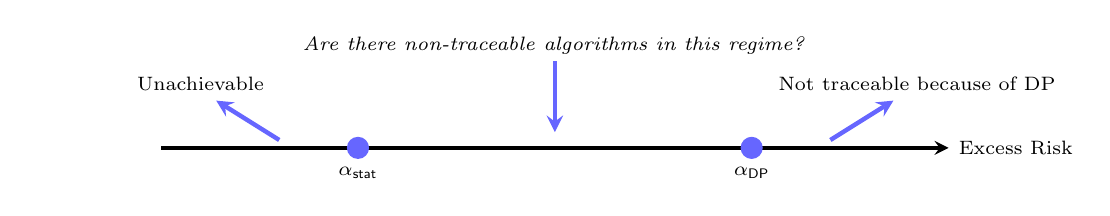
\begin{tikzpicture}[>=stealth, thick]

%
\draw[->, very thick] (-5,0) -- (5,0);

%
%
\node[anchor=west, font=\scriptsize] at (5,0){Excess Risk};

%
\fill[blue!60] (-2.5,0) circle (4pt);
\fill[blue!60] (2.5,0) circle (4pt);

%
\node[ font=\scriptsize] at (-2.5,-9pt){$\alpha_{\mathsf{stat}}$};
\node[above, font=\scriptsize] at (-4.5,0.6) {Unachievable};

%
\node[ font=\scriptsize,] at (2.5,-9pt) {$\alpha_{\mathsf{DP}}$};
\node[above, font=\scriptsize] at (4.6,0.6) {Not traceable because of DP};

%
\node[align=center, font=\scriptsize] at (0,1.3) 
{\emph{Are there non-traceable algorithms in this regime?}};
%

%
\draw[->, ultra thick, blue!60] (0,1.1) -- (0,0.2);

%
\draw[->, ultra thick, blue!60] (-3.5,0.1) -- (-4.3,0.6);
\draw[->, ultra thick, blue!60] (3.5,0.1) -- (4.3,0.6);

%
\phantom{\node[anchor=east, font=\scriptsize] at (-5,0){Excess Risk};}

\end{tikzpicture}
\vspace{-1.1em}
\caption{The various regimes for the excess risk and the main question of this paper.}
\label{fig:intro-mem}
\end{figure}

\subsection{Contributions}

\subsubsection{Tradeoff between Excess Risk and Traceability}

In this paper,  we establish a tradeoff between traceability and excess risk for algorithms in the context of SCO in general geometries.  We give informal statements of our main results below, and give a summary in~\cref{tab:trace}.

\paragraph{Tracing when \texorpdfstring{$p \in (1,2]$}{p in (1,2]}.} For the case $p\in (1,2]$, we show that every learner that obtains logarithmically better error than $\alpha_\text{DP}$ must memorize its samples, and provide essentially the best possible lower bound on the number of samples memorized. In more detail, %
we show that there exists an $\ell_p$-SCO problem such that, if an algorithm that achieves risk %
    \[\alpha \lesssim\frac {\alpha_{\mathsf{DP}}}{\log^2(n)},\]
    then $\Omega(1/\alpha^2)$ of its sample points are traceable (see~\Cref{thm:lp-traceability} for the exact statement). This result uncovers a fundamental dichotomy between traceability and privacy in $\ell_p$-SCO. It is known that $p \in (1,2]$, $\Theta(1/\alpha^2)$ is precisely the sample complexity (that is, the minimal number of samples a learner requires to achieve excess risk of $\alpha$) of learning $\ell_p$-Lipschitz problems~\citep{agarwal2009information}. Thus, any sample-efficient learner that obtains logarithmically better error than $\alpha_\text{DP}$ must memorize \emph{a constant fraction} of its sample. Note that $\Omega(1/\alpha^2)$ is essentially the best possible lower bound on recall, as there are algorithms that learn using $O(1/\alpha^2)$ samples. Hence, this result shows that a phase transition occurs: for $\alpha \ge \alpha_\text{DP}$, there are algorithms that are not $1$-traceable, and for $\alpha \lesssim \alpha_\text{DP}/\log^2(n)$, every algorithm is $\Omega(1/\alpha^2)$-traceable. ($\alpha_\text{DP}$ in this regime is known due to results in \citep{bassily2019private,asi2021private,bassily2021non}.)

\paragraph{Tracing when \texorpdfstring{$p=1$}{p = 1}.} The above result also applies to $p = 1$. However, note that, for $p = 1$, the sample complexity of learning is $\Theta(\log(d)/\alpha^2)$ \citep{agarwal2009information}, i.e., the above result only shows $1/\log(d)$ fraction of the sample can be traced in this setting. We derive a tighter version of the above result for $p = 1$, which intuitively shows that slightly more accurate learners in $\ell_1$-SCO must still memorize a constant fraction of their sample. Specifically, we show that for $p=1$ there exists an SCO problem such that, \svedit{if an algorithm achieves risk 
    \[\alpha 
    \lesssim 
    \frac{\alpha_{\mathsf{DP}}} {d^{0.01} \log^2(n)},
    \]
then $\Omega(\log(d)/\alpha^2))$ of its samples} can be traced (see~\Cref{thm:l1-traceability}). The choice of the constant $0.01$ is arbitrary.

\paragraph{Tracing when \texorpdfstring{$p \in (2,\infty)$}{p in (2,infinity)}.}
The situation becomes more complex for $2 < p < \infty$, since determining the optimal excess risk of DP learning in this setting is an open problem~\citep{bassily2019private,arora2022differentially,lee2024powersamplingdimensionfreerisk}. Nevertheless, in this setting, \svedit{we show an existence of a risk threshold below which any sample-efficient learner must again memorize a constant fraction of its samples. In more detail,}~\Cref{thm:lp-traceability-large-p} uncovers that, 
for 
    \[\alpha \lesssim \frac{\underline{\alpha}_{\mathsf{DP}}}{ \log(n)}, \] 
where $\underline{\alpha}_{\mathsf{DP}}$ is set as 
\[\underline{\alpha}_{\mathsf{DP}} = \Theta\left( \frac{d}{n^2}\right)^{1/p},\]
we can construct an SCO problem such that, if a learner achieves a risk of $\alpha$, then $\Omega(1/\alpha^p)$ of its samples are traceable. Note that, in the regime $\varepsilon \in \Theta(1)$, $\alpha_\mathsf{stat} \ll \alpha_\mathsf{DP}$ only when $d \in \Omega(n)$; in this regime, the sample complexity of learning for $p > 2$ is precisely $\Theta(1/\alpha^p)$, i.e., the number of traced out samples is again on the order of the sample complexity.

Note that $\underline{\alpha}_{\mathsf{DP}}$ need not be the optimal DP risk in this setting. Nevertheless, this quantity can be shown to be a \emph{lower bound} on the optimal DP risk (in the regime $\varepsilon \in \Theta(1)$). We extend this result to other regimes of $\varepsilon$, and another important contribution of our work is proving such DP lower bounds. 

\begin{table}
    \centering
\begin{tabular}{@{}ccc>{\centering\arraybackslash}m{1.9cm}>{\centering\arraybackslash}m{2.05cm}c@{}} 
    \toprule
     $p$ & Recall & Range of $ \alpha$ & Sample complexity & Minimax DP rate & Refs.\\
 \midrule
$1$ & $ \frac{\log(d)}{\alpha^2}$ & $ \left(\sqrt{\frac{\log(d)}{n}},\ \frac{d^{0.49}}{n \sqrt{\log(1/\xi)}}\right)$ & $\frac{\log(d)}{\alpha^2}$ &  $\sqrt{\frac{\log(d)}{n}} + \frac{\sqrt{d}}{\varepsilon n}$ &  Thm.~\ref{thm:l1-traceability}\\
 \midrule 
 $(1,2]$ & $ \frac{1}{\alpha^2}$ & $ \left(\sqrt{\frac{1}{n}},\ \frac{\sqrt{d}}{n \sqrt{\log(1/\xi)}}\right)$ & $ \frac{1}{\alpha^2}$ &  $\frac{1}{\sqrt{n}} + \frac{\sqrt{d}}{\varepsilon n}$ & Thm.~\ref{thm:lp-traceability} \\
 \midrule
 $[2,\infty)$ & $\frac{1}{\alpha^p}$ & $ \left(\min\left\{\frac{1}{n^{1/p}}, \frac{d^{1/2 - 1/p}}{\sqrt{n}}\right\}, \  \left(\frac{d}{n^2 \log(1/\xi)}\right)^{1/p}\right)$ & $\hphantom{^\dagger}\frac{1}{\alpha^p}^{\svedit\dagger}$ & \text{Open} & Thm.~\ref{thm:lp-traceability-large-p}\\
 \bottomrule
\end{tabular}
\vspace{5pt}
    \caption{Summary of traceability results. \svedit{All results are stated up to constants.} %
    The sample complexity bounds are implied by~\cref{thm:minimax-lp-rates}. Minimax DP rates are known due to~\cite{bassily2019private,bassily2021non,asi2021private,gopi2023private} and are displayed up to $\log$ factors and with $\delta = 1/n^2$. \svedit{($\dagger$) Although, in general, the sample complexity in this setting is a minimum of two terms, within the stated range of $\alpha$, the term $1/\alpha^p$ dominates.}   } 
    \label{tab:trace}
\end{table}

\subsubsection{Tighter Lower Bounds for \texorpdfstring{$\ell_p$}{Lp} DP-SCO for \texorpdfstring{$p>2$}{p greater than 2}}

Our proof techniques have implications for the sample complexity of DP-SCO. We provide an improved lower bound on DP-SCO under $\ell_p$ geometries for $p>2$ in the high dimensional regime, i.e., $d \geq \varepsilon n$, which is arguably the most interesting regime as it is more relevant for the modern ML applications. Specifically, we show, in~\Cref{thm:lp-dpsco-lb}, that for all $\varepsilon < 1$ and small $\delta$ we can construct a problem such that for every $(\varepsilon,\delta)$-DP algorithm, $\Alg_n$, there exists a data distribution such that:
    \[
    {\E_{S_n \sim \Dist^{\otimes n},\hat \param \sim \Alg_n(S_n)}\left[ \poprisk(\hat \param)\right] - \inf_{\param \in \parspace} \poprisk(\param)  \gtrsim 
    {\left(\frac{d}{n^2 \varepsilon^2}\right)^{1/p}}.}
    \]
In particular, the above implies that when $d \ge \varepsilon n$, the error due to privacy dominates the statistical error. This result improves upon all previous best bounds in the literature when $d \ge \varepsilon n$ \citep{arora2022differentially,lee2024powersamplingdimensionfreerisk}. In particular, Theorem 3.1 of~\cite{lee2024powersamplingdimensionfreerisk} gives a lower bound
   $
   \sqrt{d / n^2 \varepsilon^2},
   $
   which is weaker than our lower bound for any $p > 2$. Corollary 4 of~\cite{arora2022differentially} gives a lower bound
    $
    \min\left\{\left(\frac{1}{\varepsilon n}\right)^{\frac{1}{p}} , \frac{d^{1 - 1/p}}{\varepsilon n}\right\}
    $
    which is weaker than our lower bound for $d \ge \varepsilon n$. 
    
\subsubsection{DP and traceability in PAC Learning}
\label{sec:threshold}

Our results for SCO imply that any algorithm with an excess risk smaller than what is possible with DP is traceable with a recall that scales with the sample complexity.  A natural question is whether the same phenomenon holds true for other learning setups. 
Consider PAC classification. We show that, for every class with VC dimension bounded by $d_\mathsf{vc}$, recall of any tracer is in $O(d_{\mathsf{vc}}\log^2(n))$, i.e., it is at most a small fraction of the training sample provided $n \gg d_\mathsf{vc}$.
Many of these classes are not privately learnable, specifically, those with infinite Littlestone dimension~\cite{bun2015differentially,alon2019private,bun2020equivalence}, e.g., the class of thresholds. In other words, the sharp dichotomy between privacy and traceability does not hold in PAC classification. We also point out that for the class of thresholds, we can remove the $\log^2(n)$ factor from the recall upper bound. See~\Cref{appx:thresh} for a formal statement and further discussion.

\subsection{Related Work}

In this section, we discuss the prior work and put this paper in the context of existing results. 

\paragraph{Necessity of memorization in learning.} 
Our work is most similar in spirit to the works of~\citet{dwork2015robust} and~\citet{attias2024information}. In \cite{dwork2015robust}, the authors studied the traceability of algorithms for mean estimation in $\ell_\infty$ norm. In particular, they demonstrated that, in the accuracy regime where DP learning is impossible, every algorithm is traceable with large recall. 
More recently,~\cite{attias2024information} showed that a similar conclusion holds for learners in SCO in $\ell_2$ geometry. Our work builds on top of these results on a number of fronts. Our first novelty is a generic traceability theory (outlined in~\Cref{sec:technical}) that allows to seamlessly convert fingerprinting lemmas into traceability results and DP lower bounds. 
Another key difference is the structure of hard problems and the novelty of fingerprinting lemma. First, in our fingerprinting lemmas, the parameters of the priors in our constructions necessarily need to \emph{scale} with the risk level, in order to show that the number of memorized samples is the same as sample complexity. 
We emphasize that this scaling is indeed necessary to achieve an optimal result. For example, in the context of SCO in $\ell_2$ geometry, one could hope to use the fingerprinting lemma with \emph{uniform prior} from~\cite{dwork2015robust} along with the reduction in~\cite[Sec.~5.1]{bassily2014private}; however, it would only yield a recall of $\Omega(1/\alpha)$ samples, while the sample complexity is $\Theta(1/\alpha^2)$.  Second, $\ell_p$-SCO with $p > 2$ is distinct in the sense that the hardest problems have a sparse structure (see~\cite{agarwal2009information}). It is different from the usual constructions for mean estimation and $\ell_2$-SCO for which a ``hypercube-like'' construction suffices.  These differences necessitate new techniques, leading us to devise novel constructions and a new fingerprinting lemma specifically suited to sparse data vectors, which can be of independent interest.

A parallel line of work investigated memorization using the notion of \emph{label memorization} in supervised setups.
As per this definition, a learner is said to memorize its training samples if it ``overfits'' at these points.~\citet{feldman2020does} showed that, in some classification tasks, if the underlying distribution is \emph{long-tailed}, then a learner is forced to memorize many training labels.~\citet{cheng2022memorize} showed this phenomenon also occurs in the setting of linear regression. While this framework is suitable to study memorization in supervised tasks, the notion of ``labels'' in SCO in not well-defined and thus calls for alternative definitions.

Another line of work studied memorization through the lens of information theoretic measures. \citet{brown2021memorization} used \emph{input-output mutual information} (IOMI) as a memorization metric and showed that IOMI can scale linearly with the training sample's entropy, indicating that a constant fraction of bits is memorized. 
In the context of SCO in $\ell_2$ geometry, lower bounds on IOMI have been studied in \cite{haghifam23limitations,livni2024information}. Specifically~\cite{livni2024information} demonstrated that, for every accurate algorithm, its IOMI must scale with dimension $d$. Our approach to the study of memorization is conceptually different since we focus on the number of \emph{samples} memorized as opposed to the number of \emph{bits}. 
Nevertheless, it can be shown using~\Cref{lemma:threshold-tracing} and~\cite[Thm.~2.1]{haghifam2020sharpened} that the recall \emph{lower bounds} IOMI of an algorithm (provided that FPR $\xi$ is small enough, e.g., $\xi = 1/n^2$). However, because of the Lipschitzness of loss functions in $\ell_p$-SCO, we can use discretization of $\Theta$ and design algorithms with IOMI that is significantly smaller that the entropy of the training set, thus, memorization in the sense of \cite{brown2021memorization} does not arise here. 

\paragraph{Membership inference.} Membership inference is an important practical problem \citep{homer2008resolving, shokri2017membership, carlini2022membership}. In these works, the focus is on devising strategies for the tracer in modern machine learning settings, particularly neural networks. Our work takes a more fundamental perspective, aiming to determine whether membership inference is inherently unavoidable or simply a byproduct of specific training algorithms. An interesting aspect of our results is that, for $1 < p \le 2$, the optimal strategy for tracing depends \emph{only} on the loss function, which is in line with empirical studies~\citep{sablayrolles2019white}. 



\paragraph{Private Stochastic Convex Optimization.}
DP-SCO has been extensively studied in $\ell_2$ geometry (see, for instance, \citep{chaudhuri2011differentially,bassily2014private,bassily2019private,feldman2020private}). For $\ell_p$ with $p \in [1,2)$, the optimal DP excess risk was established in \citep{asi2021private,bassily2021non}. The best known upper bounds for DP-SCO in $\ell_p$ geometry for $p>2$ are due to \citep{bassily2021non,gopi2023private}. In this setting, there is a long-standing gap between upper and lower bounds, and the best known lower bounds are due to~\cite{arora2022differentially,lee2024powersamplingdimensionfreerisk}, which our paper improves on.  

\paragraph{Fingerprinting Lemmas and DP Lower Bounds.}
Fingerprinting codes were introduced by~\cite{boneh1998collusion}. The work~\cite{ullman2013answering} was first to relate them to lower bounds on differential privacy, and they were used extensively afterwards~\citep{bun2014fingerprinting,dwork2015robust, bun2017make,steinke2017tight,kamath2018privately,cai2023score,kamath2022new,peter2024smooth}. Intuitively, fingerprinting lemmas formalize the intuition that the output of an accurate algorithm must be correlated with its training set \citep{dwork2015robust,steinke2016upper,bun2017make,steinke2017tight,kamath2018privately,cai2023score,kamath2022new,peter2024smooth}. To put our \emph{sparse fingerprinting lemma} into the context of prior work, it can be seen to generalize the results of~\citep{steinke2017tight} to sparse sets. 
Another ``sparse fingerprinting lemma'' in the literature is given by~\cite{cai2023score} to address DP lower bounds in the sparse generalized linear model. Besides visual and naming similarities, our results are distinct. Indeed, sparsity enters the lemmas in different forms: in~\cite{cai2023score} the \emph{mean vector} is sparse (and data is dense), and in our case, the mean is dense and the \emph{data vectors} are sparse. The proof techniques also differ substantially.


\section{Problem Setup and Main Results}

\label{sec:framework-results}

We begin by a preliminary overview of the standard setup of SCO~\citep{shalev2009stochastic}. An SCO problem is characterized via a triple $\scoprob = (\dataspace, \parspace, f)$, where $\dataspace$ is the data space, $\parspace$ is the parameter space, which must be convex, and $f \colon \parspace \times \dataspace \to \Reals$ is a function such that $f(\cdot, z)$ is convex for all $z \in \dataspace$. We will assume $\parspace  \subset \Reals^d$, and $d$ is reserved to denote the dimension of the parameter space. 

In SCO, data points are drawn from an underlying distribution $\Dist$ over $\dataspace$, unknown to the learner. The objective of the learner is to minimize the \emph{expected risk} based on observed samples. More formally, assuming $\mathcal Z$ is equipped with an implicit $\sigma$-algebra, let $\mathcal M_1(\mathcal Z)$ denote the set of probability measures over $Z$. Then, a learning algorithm $\Alg_n \colon \dataspace^n \to \ProbMeasures{\parspace}$ receives a sample $S_n = (Z_1,\ldots,Z_n)$ of $n$ data points from $\dataspace^n$ and returns a (perhaps randomized) output in $\parspace$. Then, for $\Dist \in \ProbMeasures{\dataspace}$, expected risk is defined as $F_\Dist(\param) \defeq \E_{Z\sim \Dist} \left[f (Z, \param)\right].$ An $\alpha$-learner is defined to be a learner whose expected \emph{excess risk} is bounded by $\alpha$. A formal definition is given below.

\begin{definition}[$\alpha$-learner]
\label{def:alpha-learner}
Fix $\alpha > 0$, $n \in \Naturals$ and SCO problem $(\parspace,\dataspace,f)$. We say $\Alg_n:\dataspace^{n}\to \ProbMeasures{\parspace}$ is an $\alpha$-learner for $(\parspace,\dataspace,f)$ iff for every $\Dist \in \ProbMeasures{\dataspace}$, we have 
\[
\E_{S_n \sim \Dist^{\otimes n},\hat \param \sim \Alg_n(S_n)} \left[ \poprisk(\hat \param)\right] - \inf_{\param \in \parspace} \poprisk(\param)\leq \alpha
 .\]
\end{definition}

In our work, we focus on learning \emph{Lipschitz-bounded} families of problems, which are defined below. For every $p \in [1,\infty]$, let $\mathcal{B}_p(r)=\{\theta \in \Reals^d: \norm{\theta}_p\leq r\}$ be the unit ball in $\ell_p$ norm. 
\begin{definition}[Lipschitz-bounded problems] \label{def:lip-bdd}
 Fix $p\in [1,\infty]$, and let $d < \infty$ be a natural number. We let $\lipset_{p}^d$ denote the set of all $\ell_p$-Lipschitz-bounded SCO problems in $d$ dimensions. Namely, $\mathcal P = (\parspace, \dataspace, f)\in \lipset_{p}^d$ iff (i) $\parspace \subset \mathcal B_{p}(1)$, and (ii) for every $\param_1,\param_2\in \parspace$ and $z \in \dataspace$, we have 
 $|f(z,\theta_1)-f(z,\theta_2)|\leq \norm{\theta_1 - \theta_2}_p$. 
\end{definition}

\subsection{Tracing} 
\label{sec:tracing}
The key notion we study here is \emph{tracing}, and we next introduce our framework for traceability. The form of tracers discussed in the introduction takes as input the output of an algorithm and a data point and outputs a binary decision: \textsc{In} or \textsc{Out}. In the remainder of the paper, we consider families of tracers that output a real-valued \emph{score} (instead of a binary value) that intuitively corresponds to the likelihood of the event that the learner saw a data point during training. 
The binary decisions (\textsc{In} or \textsc{Out}) will then be obtained by thresholding the value of the score. Drawing parallels with hypothesis testing, this is similar to thresholding the log-likelihood ratio to obtain optimal binary tests in the Neymann--Pearson lemma. Below, we give the most general definition of a tracer.
\begin{definition}[Tracer] \label{def:tracer-def}
Fix data space $\dataspace$ and parameter space $\parspace$. A tracer's strategy is a tuple of $\tracer = (\trfn,\Dist)$ where $\trfn: \parspace \times \dataspace \to \Reals$ and $\Dist\in \ProbMeasures{\dataspace}$.
\end{definition}
In the next definition, we define the traceability of learning algorithms using the tracers in~\Cref{def:tracer-def}.
\begin{definition}[$(\xi,m)$-traceability]
\label{def:soundness-recall}
Let $n \in \Naturals$, $\xi \in (0,1)$, and $m \in \Naturals$. We say a learning algorithm $\Alg_n$ is $(\xi,m)$-traceable if there exists a tracer $(\trfn,\Dist)$ and $\lambda \in \Reals$ such that, 
if $(Z_0,Z_1,\dots,Z_n)\sim \Dist^{\otimes (n+1)}$
and $\hat \param \sim \Alg_n(Z_1,\dots,Z_n)$, 
we have
\begin{enumerate}[(i)]
\item \myul{False-positive rate (FPR):} $\P\big(\trfn(\hat{\param},Z_0)\geq \lambda\big)\leq \xi$,
\item \myul{Recall:} $\E\big[\big|\{i \in [n]:\trfn(\hat \param,Z_i)\geq \lambda\}\big|\big]\geq m$.
\end{enumerate}
\end{definition}

\subsection{Main Results}

\label{sec:main}

\subsubsection{Traceability of \texorpdfstring{$\alpha$}{alpha}-Learners}
In this section, we discuss our traceability results for accurate learners in $\ell_p$ geometries. First, we will state a result that applies to $p \in [1,2)$, and then present its slight refinement for $p = 1$. We will then present our result for $p \ge 2$. See~\Cref{pf:thm:lp-traceability,pf:thm:l1-traceability,pf:thm:lp-traceability-large-p} for proofs.%

\begin{restatable}{theorem}{LPTraceability}
\label{thm:lp-traceability}
    There exists a universal constant $c>0$ such that, 
    for all $p \in [1,2)$, if $d$, $n$, $\xi \in (0, 1/e)$, and $\alpha > 0$ are such that
    \svedit{\begin{equation} \label{eq:l-p-tracing-cor-condition-eps} 
    \frac{c}{\sqrt{n}} \le \alpha \le {\min\left\{c \cdot \sqrt{\frac {d} {n^2 \log(1/\xi)}}, \  \frac{1}{6}\right\}}, 
    \end{equation} 
    then} there exist an $\ell_p$-Lipschitz-bounded problem such that \myul{every} $\alpha$-learner is $(\xi, m)$-traceable with 
    $
    m \in \Omega\left(\alpha^{-2}\right).
    $
\end{restatable}
\svedit{Note that the upper bound on $\alpha$ in~\cref{eq:l-p-tracing-cor-condition-eps} is precisely the optimal DP excess risk for $\varepsilon \in \Theta(1)$ and $p \in [1,2]$~\citep{asi2021private,bassily2021non}, and the lower bound is precisely the optimal non-private risk (except $p = 1$; see~\cref{thm:minimax-lp-rates}).} Moreover, for $p \in (1,2]$, the lower bound on $m$, i.e., the number of memorized samples, \emph{exactly} matches the sample complexity of $\ell_p$-SCO problems. 
For $p = 1$, this bound is less than the sample complexity by a factor of $\log(d)$. (See~\Cref{cor:sample-cmplx-lb} for an overview of known rates for the sample complexity of SCO.) 
Thus, our result uncovers a dichotomy for $p \in [1,2]$: every algorithm with excess risk \emph{better} than the optimal DP excess risk is traceable with a recall that scales with the sample complexity. 

As mentioned above, for $p = 1$, the lower bound on recall in~\cref{thm:lp-traceability} is less than sample complexity by a factor of $\log(d)$. This prompts us to establish the following refinement for $p=1$.
\begin{restatable}{theorem}{LOneTraceability}
\label{thm:l1-traceability}
    There exists a universal constant $c>0$ such that, if $d$ \svedit{is large enough} and $n$, $\xi \in (0, 1/e)$, and $\alpha > 0$ are such that  \svedit{\begin{equation}
    c\cdot \sqrt{\frac{\log(d)}{n}} \le \alpha \le { 
    \min \bigg\{c\cdot \frac{d^{0.49}}{n \sqrt{\log(1/\xi)}} , \frac{1}{8}\bigg\},
    }
    \label{eq:l-1-trace-condition-eps}\end{equation} 
    there} exists an $\ell_1$-Lipschitz-bounded problem such that \myul{every} $\alpha$-learner is $(\xi, m)$-traceable with 
    $
    m \in \Omega\left(\log(d)/\alpha^2\right).
    $
\end{restatable}
Note that the upper bound in~\cref{eq:l-1-trace-condition-eps} is slightly stronger than in~\cref{eq:l-p-tracing-cor-condition-eps}; however, the lower bound on recall now matches the sample complexity of learning in $\ell_1$ geometry. We now present a result for $p > 2$.

\begin{restatable}{theorem}{LPTraceabilityLargeP}
\label{thm:lp-traceability-large-p}
    There exists a universal constant $c>0$ such that, 
    for all $p \in [2,\infty)$, if $d$, $n$, $\xi \in (0, 1/e)$, and $\alpha > 0$ are such that
    \svedit{\begin{equation} \label{eq:l-p-tracing-cor-condition-eps-large-p} 
    \frac{1}{6} \cdot \min\left\{ \frac{1}{n^{1/p}}, \ \frac{d^{\frac{1}{2} - \frac{1}{p}}}{\sqrt{n}}\right\} \le \alpha \le {\min\left\{c \cdot \left(\frac {d} {n^2 \log(1/\xi)}\right)^{1/p}, \  \frac{1}{6}\right\}}, 
    \end{equation} 
    then} there exist an $\ell_p$-Lipschitz-bounded problem such that \myul{every} $\alpha$-learner is $(\xi, m)$-traceable with 
    \[ m \in \Omega\left(\frac{1}{(6\alpha)^p}\right).\]
\end{restatable}

For $p \in (2,\infty)$, our results have a different implication, showing that all sufficiently accurate learners need to memorize a number of samples on the order of the sample complexity. 
However, in this case, \svedit{the upper bound in}~\cref{eq:l-p-tracing-cor-condition-eps-large-p} need not be the optimal DP error. Instead, it provides a \emph{lower bound} on the optimal DP error, as we will see shortly (\cref{thm:lp-dpsco-lb}). 
%
%
We note that $p = \infty$ is excluded from the range above, because $\alpha_\mathsf{DP} \in O(\alpha_\mathsf{stat})$ 
in $\ell_\infty$~\cite{bassily2021non}. As mentioned in the introduction, the question of traceability is vacuous unless $\alpha_\mathsf{stat}$ and  $\alpha_{\mathsf{DP}}$ are sufficiently far apart.  

\svedit{\begin{remark}
    We make a brief remark on the lower bounds in~\cref{eq:l-1-trace-condition-eps,eq:l-p-tracing-cor-condition-eps,eq:l-p-tracing-cor-condition-eps-large-p}. Note that these lower bounds precisely correspond to minimax excess risk of learning $\ell_p$-Lipschitz-bounded classes for appropriate values of $p$ (see~\Cref{thm:minimax-lp-rates}). Also, in the proofs of these theorems, the problems we consider are \emph{the hardest} problems to learn within each respective class (see~\Cref{thm:sparse-family-sample-complexity,thm:l1-family-sample-complexity}). Thus, for each of these problems, if there exists an $\alpha$-learner, then $\alpha$ automatically satisfies the lower bound in~\cref{eq:l-1-trace-condition-eps,eq:l-p-tracing-cor-condition-eps,eq:l-p-tracing-cor-condition-eps-large-p} (up to constants). I.e., the question of traceability is vacuous whenever this lower bound is not satisfied. 
\end{remark}}

\subsubsection{Improved DP-SCO Lower Bound for \texorpdfstring{$p>2$}{p greater than 2}}
While our focus has been on tracing, we have developed several technical tools that are of independent interest.  
As our next theorem shows, using the notion of trace value, which we further develop in subsequent sections, we show improved lower bounds for DP-SCO in $\ell_p$ geometries for $p > 2$. The proof 
can be found in~\Cref{pf:thm:lp-dpsco-lb}.
\begin{restatable}{theorem}{LpDPSCO}
\label{thm:lp-dpsco-lb}
    Let $p \in [2,\infty)$ be arbitrary. Then, there exist a universal constant $c>0$ and a problem $\scoprob = (\parspace,\dataspace,\ell) \in \lipset_{p}^d$ 
    such that any $(\varepsilon,\delta)$-DP learner of $\mathcal P$ with $\varepsilon \le 1$ and $\delta \le c/n$ satisfies,
    \[
    \alpha \ge c \cdot {\min\bigg\{ \left(\frac{d}{\varepsilon^2 n^2}\right)^{\frac{1}{p}} , \frac{d^{1-1/p}}{\varepsilon n} , 1 \bigg\}}.  
    \]

\end{restatable}

\section{Technical Overview}

\label{sec:technical}

Our proofs rely on introducing two key technical elements that allow us to generalize tracing techniques to general $\ell_p$ setups. 
The first elements is a novel complexity notion which we term \emph{the (subgaussian) trace value} of a problem. Surprisingly, as we show in the proof of~\Cref{thm:lp-dpsco-lb}, we can use the trace value not only to prove traceability results, but also to establish DP sample complexity lower bounds, and, even to recover  \emph{non-private} sample complexity lower bounds.


The subgaussian trace value is defined by narrowing down the general family of tracers and additionally requiring that the tracer $(\trfn,\Dist)$ induces a subgaussian process over the set $\Theta$ (which we formalize shortly).
To provide intuition behind this requirement, the subguassianity assumption on the tracer let us argue that (i) if $\hat \theta$ was not trained on $Z \sim \Dist$, then $\trfn(\hat \theta, Z)$ will be small with high probability, and, (ii)  $\sup_{\param \in \parspace} \sum_{i = 1}^n \left[\trfn(\param, \datapt_i) \right]^2$ is bounded with high probability.
As per~\Cref{def:soundness-recall}, condition (i) ensures a small FPR of a tracer, and condition (ii) is useful for the following technical reason. It allows us to argue that, if the trace value is large on average over the training set, it implies the existence of a threshold $\lambda$ such that $\trfn(\hat \theta, Z)\ge\lambda$ for many $Z \in S_n$, and thus establishing recall.

Our second technical contribution concerns techniques for lower bounding the trace value, which we accomplish through several novel \emph{fingerprinting lemmas}.
Previous works used the standard fingerprinting lemma, where the learner observes points on a hypercube, to lower bound DP and traceability in $\ell_2$ geometry. However, when moving to general $\ell_p$ geometries, this setup no longer captures the hardest settings to learn. For instance, for $p > 2$, canonical instances of hard problems involve data drawn from sparse sets~\citep{agarwal2009information}. 
We thus prove new fingerprinting lemmas that enable us to leverage our framework in such settings. These fingerprinting lemmas are then applied to carefully constructed instances of hard problems, and we show that every accurate learner of these problems is traceable. In the remainder of this section, we provide a formal definition of trace value, subgaussian processes, and state our new fingerprinting lemmas.  Then, we show the notion of trace value lets us reason about tracing, DP, and (even) non-private sample complexity lower bounds.

\subsection{General framework: subgaussian trace value} 
\label{sec:framework}

We next describe more formally the framework of subgaussian tracers. For a random variable $X$, 
the subgaussian norm of $X$
is the quantity 
$
\gaussnorm{X} \defeq \inf\{t\colon \E \left[ \exp(X^2/t^2)\right] \le 2\}
$
\citep{vershynin2018high}.
We use the following definition of a subgaussian process:
\begin{definition}[Subgaussian process]
\label{def:subg-process}
    We call an indexed collection of random variables $\{X_\param\}$ a $\sigma$-subgaussian process w.r.t a metric space $(\parspace,\norm{\cdot})$ if for every $\param, \param' \in\parspace$, we have
    \[
    \gaussnorm{X_{\param} - X_{\param'}} \le \sigma \norm{\param - \param'}, \quad \gaussnorm{X_\param} \le \sigma \diam_{\norm{\cdot}} (\parspace).
    \]
\end{definition}
For origin symmetric convex body $\Theta$, let $\norm{\cdot}_\Theta$ denote the Minkowski norm w.r.t. $\Theta$, that is $\norm{x}_\Theta := \inf\left\{ \lambda > 0\colon x \in \lambda \Theta \right\}.$
If $\Theta$ is not convex or not origin symmetric, we let $\norm{\cdot}_\Theta$ be the Minkowski norm w.r.t. convex hull of $(\Theta \cup -\Theta)$. Note that $\norm{\cdot}_\Theta$ is the minimal norm to contain $\Theta$ in its unit ball. Then, a subgaussian process naturally leads to a definition of a subgaussian tracer as follows.




\begin{definition}[Subgaussian tracer] \label{def:subg-tracer}
Fix $\kappa \in \Reals$ to be a constant, and let $\Theta$ be a convex body. We let $\tracerset_\kappa$ be the class of subgaussian tracers at scale $\kappa > 0$, that is, a tracer $(\trfn,\Dist) \in \tracerset_\kappa$ iff
\begin{enumerate}[(i)]
    \item $\{\trfn(\theta,Z)\}_{\theta \in \Theta}$ where $Z \sim \Dist$ is a $1$-subgaussian process w.r.t. $(\Theta, \norm{\cdot}_\Theta)$.
    \item $|\trfn(\theta, z)| \le \kappa$ for all $\theta \in \Theta$ and $z\in\dataspace$. 
    \item $\trfn(\cdot, z)$ is convex for all $z\in\dataspace$.
\end{enumerate}
\end{definition}
We make a note in passing that the convexity condition is necessary only for $\ell_1$-proofs.

\begin{definition}[Subgaussian trace value]\label{def:trace-value}
Fix $n \in \Naturals$, $\alpha\in [0,1]$, and $\kappa \in \Reals$. Consider an arbitrary SCO problem $\scoprob = (\parspace,\dataspace,f)$. Let $\tracerset_\kappa$ be as in~\Cref{def:subg-tracer}.
Then, we define the subgaussian trace value (or trace value in short) of problem $\scoprob$ by
\[
\traceval_\kappa(\scoprob;n,\alpha) = \inf_{ \alpha\text{-learner} \Alg_n}~\sup_{\tracer=(\trfn,\Dist) \in \tracerset_\kappa}~ 
{\E_{S_n=(Z_1,\dots,Z_n) \sim \Dist^{\otimes n}, \hat \theta \sim \Alg_n(S_n)} \bigg[\frac{1}{n}\sum_{i\in [n]} \trfn(\hat \theta,Z_i)\bigg]} .
\]
where the $\inf$ is taken over all $\Alg_n$ that achieve excess risk $\le \alpha$ on $\mathcal P$ with $n$ samples. 
\end{definition}

\paragraph{Traceability via trace value.}

The trace value characterizes the average score the pair $(\trfn, \Dist)$ assigns to the data points in the training set. 
However, the definition of recall in~\Cref{def:tracer-def} requires characterizing the \emph{number} of samples in the training set that takes a large value. The former can be converted into the latter, provided the sum of squared scores of samples is not too large. A formal statement, which is a consequence of Paley–Zygmund inequality, can be found in~\Cref{lem:card-moments}.
In the next lemma, we show how to control the sum of squares of the $\trfn(\hat \theta,Z_i)$ using the subgaussian assumption we made on $\trfn$. The main machinery used for proving the lemma is  Dudley's entropy integral to control the supremum of a subgaussian process. 
\begin{restatable}{lemma}{LemmaSubgProcess}
    \label{lemma:subg-process}
    Fix $n,d \in \Naturals$. Suppose $\parspace \subset \Reals^d$ is a subset of a unit ball in some norm $\norm{\cdot}$. Let $\trfn \colon \parspace \times \dataspace \to \Reals$ and $\Dist \in \ProbMeasures{\dataspace}$ be such that, as $Z \sim \Dist$, $\{\trfn(\param, \datapt)\}$ is a $\sigma$-subgaussian process w.r.t. $(\parspace,\norm{\cdot})$.
    Let $(Z_1,\dots,Z_n)\sim \Dist^{\otimes n}$.   Then, there exists a universal constant $C> 0$, such that 
    \[
    \P\left[\sup_{\param \in \parspace} \sqrt{ \sum_{i = 1}^n \left[\trfn(\param, \datapt_i) \right]^2} \le C \sigma \left(\sqrt{n} + \sqrt{d} + t\right)\right]\geq 1 - 4\exp(-t^2), \quad \forall t \ge 0.
    \]
\end{restatable}
In the next theorem, we show that~\Cref{lemma:subg-process} implies that if, the trace value is large, it means that for \emph{many} in-sample data points $Z_i$, the value of $\trfn(\hat \theta, Z_i)$ is large, which allows the tracer to reliably identify $Z_i$ as part of the training set. Additionally, for a fresh sample $Z_0 \sim \Dist$, $\trfn(\hat\theta, Z_0)$ will be small with high probability, once again due to the subgaussian assumption.
\begin{restatable}{theorem}{TheoremMasterTracing}
\label{thm:master-tracing}
     Fix $n \in \Naturals$, $d \in \Naturals$, $\kappa > 0$ and $\alpha\in [0,1]$.  Consider an arbitrary SCO problem $\scoprob = (\parspace,\dataspace,f)$. Let $T = \traceval_\kappa(\scoprob;n,\alpha)$ be the trace value of $\scoprob$.
     Then, for some constant $c > 0$, every $\alpha\text{-learner}~\Alg_n$ is $(\xi,m)$-traceable with
     \[
     \xi = \exp(-c T^2), \quad 
     {m = c\left[\frac{n^2T^2}{n + d} - \frac{16\kappa^2 n}{\exp(n + d)}\right].}
     \]
\end{restatable}

\paragraph{Privacy lower bounds via trace value.}
In the next theorem, we show that the notion of trace value directly lower bounds the best privacy parameters achievable by a DP algorithm. The proof can be found in~\Cref{pf:thm:master-privacy-lb}.
\begin{restatable}{theorem}{TheoremMasterPrivacy}
\label{thm:master-privacy-lb}
     There exists a universal constant $c > 0$, such that the following holds. Fix $p \in [1,\infty)$, $n \in \Naturals$,  $d \in \Naturals$, $\alpha\in [0,1]$, $\kappa > 0$ $\varepsilon >0$, and $\delta \in [0,1]$.  Consider an arbitrary SCO problem $\scoprob = (\parspace,\dataspace,f)$ in $\Reals^d$.  Let $T = \traceval_\kappa(\scoprob;n,\alpha)$ be the trace value of problem $\scoprob$. Then, for any $(\varepsilon, \delta)$-DP $\alpha$-learner $\Alg_n$, we have 
    $
    \exp(\varepsilon)-1 \geq c\left(T - 2\delta \kappa\right).
    $
\end{restatable}

\paragraph{Connection to non-private sample complexity.}
    \label{remark:non-priv-sample-complexity}
    Remarkably, the trace value can also be used to lower bound the sample complexity of non-private learning. Naively, if every $\alpha$-learner is $(\xi,m)$-traceable, it implies a lower bound of $m$ on the sample complexity. However, in~\Cref{thm:lp-traceability,thm:lp-traceability-large-p,thm:l1-traceability}, \svedit{we begin by assuming that $\alpha \ge \alpha_{\mathsf{stat}}$ for the respective class of problems, i.e., any argument using~\Cref{thm:lp-traceability,thm:lp-traceability-large-p,thm:l1-traceability} to lower bound sample complexity would be cyclical.}
    %
    
    \svedit{Surprisingly, if we directly use \emph{trace value}, we can} recover optimal sample complexity bounds \emph{for all $p \in [1,\infty)$ and all regimes of $(d,\alpha)$}, thus unifying traceability with private and non-private sample complexity lower bounds. While we detail the argument formally in~\Cref{sec:sample-complexity}, we consider here a helpful example of $\ell_2$ geometry. First, it can be shown that we always have \[\traceval(\mathcal P; n,\alpha) \lesssim \sqrt{d/n}\] for arbitrary problem $\mathcal P$ (see~\cref{prop:master-sample-complexity}). Also, we will later show that, for any $\alpha > 0$, there exist an $\ell_2$ problem $\scoprob$ with \[\traceval(\mathcal P; n,\alpha) \gtrsim \sqrt{d}/n\alpha\] (see~\cref{thm:tracing-result-lp}). Combining the two inequalities and solving for $n$, we obtain $n \gtrsim 1/\alpha^2$, which is optimal. 
\subsection{Fingerprinting lemmas} 

\label{sec:fingerprinting}

By introducing the notion of trace value, we have reduced the problems of traceability and privacy lower bounds to the question of lower bounding the trace value. Now, we discuss the techniques to lower bound trace value. The proofs can be found in~\Cref{appx:fingerprinting}.

\paragraph{Sparse fingerprinting lemma.} For $\ell_2$ geometry, one can lower bound trace value using the classical fingerprinting lemma  in~\citep{dwork2015robust}. (See \citep{bassily2019private,attias2024information}). Intuitively, fingerprinting lemmas show that the correlation of the output of any algorithm to the unknown mean can be tightly related to the correlation to samples. While this strategy leads to traceability results in $\ell_2$ geometry, examples of hard problems for $\ell_p$ geometry with $p > 2$ are those with \emph{sparse} sets $\dataspace$ (e.g., as in~\citep{agarwal2009information}). This motivates us to prove the following \emph{sparse fingerprinting lemma}, which is another important contribution of our work. For a vector $x \in \Reals^d$, let $\supp(x)$ be the set of its non-zero coordinates and denote $\norm{x}_0 =|\supp(x)|$. First, we define a family of distributions over sparse sets $\dataspace$.
\begin{definition}[Sparse distributions family]
\label{def:family-dist-sparse}
Fix $d \in \Naturals$, $k \in [d]$ and $\mu \in [-k/d,k/d]^d$.
Consider the mixture distribution on
\[
\dataspace_k = \{z\in \{0,\pm 1\}^d: \norm{z}_0=k\}
\]
given by, for all $z \in \dataspace_k$,
\[
\Dist_{\mu,k}(z) = \E_{J \sim  \unif{\binom{[d]}{k}}}\left[P_{\mu,k,J}(z)\right], 
\]
where
\[
P_{\mu,k,J}(z) = 
\ind(\supp(z) = J) \cdot {\prod_{j \in J}}\left( {\frac{1 + (d/k) \cdot \mu^j z^j}{2}}\right).\]
\end{definition}
Note that, in particular, $\E_{Z \sim \Dist_{\mu,k}}[Z] = \mu$. Intuitively, one can think of \emph{sampling} from $\Dist_{\mu,k}$ using the following procedure: (i) sample the support coordinates $J \sim \mathsf{unif}\binom{[d]}{k}$, (ii) for each $j \in J$, sample $Z^j$ from $\{\pm 1\}$ with mean $\frac{d}{k}\mu^j$ independently, (iii) for each $j \not \in J$, set $Z^j=0$.

With this distribution family at hand, we may state the sparse fingerprinting lemma. For $x, y \in \Reals^d$ and a subset $R \subseteq [d]$ of coordinates, we use $\inner{\cdot}{\cdot}_S$ to denote the inner product $\inner{x}{y}_R := \sum_{i \in R} x_i y_i$. Also, for $\alpha,\beta,\gamma > 0$, let $\dbeta[{[-\gamma,\gamma]}]{\alpha}{\beta}$ be the \emph{symmetric} beta-distribution, i.e., beta distribution with parameters $\alpha,\beta$ scaled and shifted to have support $[-\gamma,\gamma]$ (see~\Cref{def:rescaled-beta-dist}).
\begin{restatable}[Sparse fingerprinting]{lemma}{LemmaSparseFingerprinting}
    \label{lemma:sparse-fingerprinting} 
    Fix $d,n \in \Naturals$ and let $k \in [d]$. For each $\mu \in [-k/d,k/d]^{d}$, let $\dataspace_k$ and $\Dist_{\mu,k}$ be as in~\Cref{def:family-dist-sparse} .
    Let $\pi = \dbeta[{[-k/d,k/d]}]{\beta}{\beta}^{\otimes d}$ be a prior and set
    \[
    \trfn_\mu(\param,Z) \defeq \inner{\param}{\left(Z - {\frac{d}{k}} \mu\right)}_{\supp\left(Z\right)}.
    \]
    Then, for every learning algorithm $\Alg_n: \dataspace^n \to \ProbMeasures{\Reals^d}$ with sample $S_n = (Z_1,\ldots,Z_n)$,   
    \[
        \E_{\mu \sim \pi} \E_{S_n \sim \Dist_{\mu,k}^{\otimes n},\hat \theta \sim \Alg_n(S_n)} \left[ {\sum_{i = 1}^n \trfn_\mu(\hat\theta,Z_i) }\right] = \frac{2\beta d}{k} \E_{\mu \sim \pi} \inner{\mu}{\E_{S_n \sim \Dist_{\mu,k}^{\otimes n},\hat \theta \sim \Alg_n(S_n)} [\hat\theta] }.
    \]
\end{restatable}

The key novelty of this lemma is that it provides a way to study the correlation between a learner's output and training samples on sparse sets $\dataspace_k$. An important and distinctive feature of this result is that the right-hand side scales by a factor of $d/k$, highlighting the fact that sparse problems correspond to greater trace values. Intuitively, this stems from the fact that each coordinate is \emph{seen} fewer times by the learning algorithm, meaning it must retain more information from each training sample in order to learn accurately. Additionally, we note that for the special case $k = d$, the result precisely recovers the fingerprinting lemma with $\beta$-priors from~\citep{steinke2017tight}.

\paragraph{Fingerprinting for \texorpdfstring{$\ell_1$}{L1} setup.} Additionally, to prove~\Cref{thm:l1-traceability}, we will need the following fingerprinting lemma. It can be seen as a generalization of beta-fingerprinting lemma in~\cite{steinke2017tight} using the scaling matrix technique of~\cite{kamath2018privately,attias2024information}. 
\begin{restatable}[Fingerprinting lemma with a scaling matrix]{lemma}{FingerprintingScalingMatrix}
\label{lemma:beta-scaling-matrix-fingerprinting}
Fix $d \in \Naturals$. Let $\dataspace = \{\pm 1\}^d$ and let $\beta > 0$ be arbitrary. Consider arbitrary $0 < \gamma \le 1$. For every $\mu \in [-\gamma,\gamma]^{d}$, let $\Dist_\mu$ be the product distribution on $\dataspace$ with mean $\mu$, i.e., for every $z\in \dataspace$, we have
\[
\Dist_\mu = \prod_{k=1}^{d} \left(\frac{1+z^k\mu^k}{2}\right)
\]
let $\Lambda_\mu$ be a diagonal matrix of size $d$ where the $i$-th diagonal element is given by
\[
\Lambda_\mu^{ii} = \frac{1 - (\mu^i/\gamma)^2}{1 - (\mu^i)^2},
\]
and let $\trfn_\mu(\theta,z) = \inner{\theta}{\Lambda_\mu (z - \mu)}$. Let $\pi = \dbeta[{[-\gamma,\gamma]}]{\beta}{\beta}^{\otimes d}$ be a prior.
Then, for any algorithm $\Alg_n: \dataspace^n \to \ProbMeasures{\Reals^d}$, we have
\[
\E_{ \mu \sim \pi} \E_{S_n\sim  \Dist_\mu^{\otimes n},\hat \theta \sim \Alg_n(S_n)}\sum_{Z \in  S_n} \trfn_\mu(\hat\theta,Z) = \frac{2\beta}{\gamma^2} 
{\E_{ \mu \sim \pi} \inner{\mu}{ \E_{S_n\sim \Dist_\mu^{\otimes n},\hat \theta \sim \Alg_n(S_n)}[\hat \theta]}.}
\]
\end{restatable}
This fingerprinting lemma is handy for the following reason. To ensure the problem is hard to learn, entries of $\mu$ typically need to \mhedit{inversely} scale with $\alpha$. To achieve this, one can select small $\gamma$ in the above to shrink the beta-prior to a smaller scale, while simultaneously having the freedom to set $\beta$ to any value. In particular, this allows us to choose $\beta \in \Theta(\log(d))$ in the proof of~\Cref{thm:l1-traceability} to leverage the anti-concentration result of \citep[Prop.~5]{steinke2017tight}.
 
\subsection{Final steps: bounding the trace value for hard problems}
\label{sec:trace-lb}
Finally, we go over the construction of hard problems. To illustrate the difficulty of problem constructions, we give an example of a problem that requires many samples to learn but nevertheless is not traceable. Specifically, we consider learning over $\ell_1$ ball with linear loss. Let \begin{equation} 
\label{eq:l1-counterexample}
\parspace = \mathcal B_1(1), \quad \dataspace = \{\pm 1\}^{d}, \quad f(\theta, Z) = - \langle \theta, Z\rangle.
\end{equation} 
Consider a difficult set of distributions $\{\Dist_i\}_{i = 1}^d$ where $\Dist_i$ is a product distribution on $\dataspace$ and has mean $\alpha$ on coordinate $i$ and mean zero on all other coordinates. It can be shown this problem requires $\Theta(\log(d)/\alpha^2)$ samples to learn up to an accuracy of $\alpha/3$, and ERM is an optimal learner. However, after seeing $\Theta(\log(d)/\alpha^2)$ samples from $\Dist_i$, the ERM takes the value $\hat \theta = e_i$ w.h.p., which is also the \emph{population} risk minimizer. In other words, it becomes impossible to trace out any specific samples on which $\hat\theta$ was trained. Intuitively, since ERM can only take $2d$ values (at the vertices of an $\ell_1$-ball), it does not carry sufficient information about the training sample. 

We first will give a generic construction that gives a lower bound on the trace value for all $p \in [1,\infty)$, and then present a refinement for $p = 1$. 

\paragraph{Generic construction.} As mentioned above, to obtain optimal results for $p > 2$, problems constructed need to be sparse, and the main subtlety in our constructions is choosing the sparsity parameter. For some $k \in [d]$ to be chosen later, consider the following $\ell_p$-Lipschitz problem $\mathcal P_{k,p}$.
\begin{equation}
\label{eq:lp-sketch-construction}
\Theta = \mathcal B_{\infty}(d^{-1/p}), \quad \mathcal Z = \{ z \in \{0,\pm 1\}^d\colon \norm{z}_0 = k \}, \quad f(\theta, z) = - k^{-1/q} \langle \theta, z \rangle.
\end{equation}
\svedit{Here, the parameter space $\Theta$ is the largest $\ell_\infty$ ball inscribed into the unit $\ell_p$ ball, and $q$ is the H{\"o}lder conjugate of $p$, i.e., $\frac{1}{p} + \frac{1}{q}=1$.} The next step is to show that $\alpha$-learners for the above problem must be correlated with the mean of the unknown data distribution. Let $\Dist$ be a distribution with mean $\mu$, and suppose $\Alg_n$ is an $\alpha$-learner for~\cref{eq:lp-sketch-construction}. Then, we can show
\[
    \E_{S_n \sim \Dist^{\otimes{n}},\hat \theta \sim \Alg_n(S_n)}\left[\inner{\mu}{\hat\theta}\right] \ge \sup_{\param\in\parspace} \inner{\mu}{\param} - k^{1/q} \cdot \alpha = d^{-1/p} \norm{\mu}_1 - k^{1/q} \alpha.
\]

Now, we apply the sparse fingerprinting lemma (\Cref{lemma:sparse-fingerprinting}). A key step is choosing the scale $\beta \ge 1$ of the beta-prior. On the one hand, $\beta$ should be small enough to guarantee $\E d^{-1/p} \norm{\mu}_1 > k^{1/q} \alpha$, so that the above lower bound is non-vacuous. On the other hand, taking $\beta$ too small decreases the sample complexity of learning the problem, thus, disallowing the desired level of recall. The optimal choice is 
$\beta \propto \alpha^{-2} \cdot (k/d)^{1/p}$, 
as long as this quantity is $\ge 1$. This choice yields
\[
    \traceval_{\kappa}(\scoprob_{k,p}; n, \alpha) \ge \E_{S_n \sim \Dist^{\otimes n},\hat \theta \sim \Alg_n(S_n)} \left[ \frac{1}{n}{\sum_{i = 1}^n } \trfn(\hat\theta,Z_i)\right] \gtrsim \frac{d^{1 - 1/p}}{k^{1/2 - 1/p} n \alpha},
\]
where $\kappa \in \Theta(1)$, and, for some universal constant $c>0$, we let
\[
\trfn(\param,Z) := \frac{cd^{1/p}}{\sqrt{k}} \inner{\param}{\left(Z - {\frac{d}{k}} \mu\right)}_{\supp\left(Z\right)}.
\]
Note that the $d^{1/p}/\sqrt{k}$ scaling ensures $\trfn$ induces a $1$-subgaussian process. Finally, it remains to choose a suitable value for $k$, for each pair $(p,\alpha)$. Recall the definition of $\mathcal P_{k,p}$ from~\cref{eq:lp-sketch-construction}.
\begin{restatable}{theorem}{TraceValueLp}
\label{thm:tracing-result-lp}
Let $\mathcal P_{k,p}$ be the family of problems described in \cref{eq:lp-sketch-construction}. There exist universal constants $c_1,c_2 >0$ such that,
   for all $\alpha \in (0, 1/6]$ and $d \in \Naturals$, the following trace value lower bounds hold for all $p \in [1,\infty)$ and $\kappa \le c_1 \sqrt{d}$:
\begin{enumerate}[(i)]
    \item For $p \le 2$ and $k = d$, we have
    \[
    \traceval_{\kappa}(\scoprob_{k,p}; n, \alpha) \ge c_2\frac{\sqrt{d}}{n\alpha}.
    \]
    \item For $p \ge 2$ and $k = (6\alpha)^p d \lor 1$, we have 
    \[
        \traceval_{\kappa}(\scoprob_{k,p}; n, \alpha) \ge c_2\left[\frac{\sqrt{d}}{n (6\alpha)^{p/2}} \land \frac{d^{1 - 1/p}}{n \alpha}\right].
    \]
    \end{enumerate}
\end{restatable}
Using the reduction~\Cref{thm:master-tracing}, the above establishes~\Cref{thm:lp-traceability,thm:lp-traceability-large-p}.

\paragraph{Refinement for \texorpdfstring{$p = 1$}{p = 1}.} While the above construction also yields a traceability result for $p = 1$, it is suboptimal for the following simple reason: for $k = d$, the problem in~\cref{eq:lp-sketch-construction} only requires $\Theta(1/\alpha^2)$ samples to learn, thus, it is impossible to trace out $\Omega(\log(d)/\alpha^2)$ samples. On the other hand, the problem in~\cref{eq:l1-counterexample} requires $\Theta(\log(d)/\alpha^2)$ samples to learn but is not traceable. The intuition we follow here is to modify the construction in~\cref{eq:lp-sketch-construction} to make $\Theta$ ``look'' more like an $\ell_1$-ball to drive up the sample complexity while still avoiding the counterexample with an ERM learner from the beginning of the section. 
In particular, we consider the following $\ell_1$-problem,
\begin{equation}
\label{eq:ell1-sketch-construction}
\Theta = \mathcal B_1(1) \cap \mathcal B_\infty(1/s), \quad \dataspace = \{\pm 1\}^d, \quad f(\theta, z) = - \langle z, \theta \rangle,
\end{equation}
for a suitably chosen $s \in [d]$. Note that, if we choose $s \gg 1$, $\Theta$ above is a polytope with much more vertices ($2^s \binom{d}{s}$) than an $\ell_1$ ball ($2d$), which would intuitively force a learner like an ERM to reveal more information about the training sample. On a technical level, selecting large $s$ improves the subgaussian constant of a tracer; however, selecting $s$ that is too large shrinks the diameter of the set, and thus, the problem becomes easier to learn. We must trade off these two aspects, and carefully set the value of $s$. As it turns out, the optimal choice is $s \propto d^{1 - c}$ for any small $c > 0$ in order to establish~\Cref{thm:l1-traceability}. 
The remainder of the proof is rather technical and hence is deferred to~\Cref{pf:thm:l1-traceability}.

\subsection{Open problem: dichotomy for \texorpdfstring{$p > 2$}{p greater than 2}.}
We conclude the technical section by stating an intriguing open problem. 
We conjecture~\Cref{thm:lp-dpsco-lb} is tight, and the dichotomy between traceability and SCO also holds for $p > 2$.  
In particular, we conjecture that the optimal DP-SCO excess risk for $\ell_p$ with $p>2$ scales as
\[
\min\left\{\frac{d^{1/2 - 1/p}}{\sqrt{n}},\left(\frac{1}{n}\right)^{1/p}\right\} + \min\left\{\frac{d^{1 - 1/p}}{n\epsilon}, \left(\frac{d}{\epsilon^2 n^2}\right)^{1/p}\right\},
\]
ignoring $\log(1/\delta)$ factors. If the conjecture is true, we have a complete understanding of traceability in SCO. If it is false, it reveals that there is something fundamentally different about settings with $p > 2$, which would also significantly enrich our understanding of DP-SCO.

\section*{Acknowledgments}
The authors would like to thank Mufan Li and Ziyi Liu for their comments on the drafts of this work. 

\section*{Funding}

\svedit{This work was completed while Sasha Voitovych was a student at the University of Toronto and supported by an Undergraduate Student Research Award from the Natural Sciences and Engineering Research Council of Canada.} Mahdi Haghifam is supported by a Khoury College of Computer Sciences Distinguished Postdoctoral Fellowship. 
Idan Attias is supported by the National Science Foundation under Grant ECCS-2217023, through
the Institute for Data, Econometrics, Algorithms, and Learning (IDEAL).
Roi Livni is supported by a Google fellowship, a Vatat grant and the research has been funded, in parts, by an ERC grant (FoG - 101116258). Daniel M.~Roy is supported by the funding through
NSERC Discovery Grant and Canada CIFAR AI Chair at the Vector Institute.

\printbibliography

\addtocontents{toc}{\protect\setcounter{tocdepth}{2}}
\renewcommand{\contentsname}{Appendix Contents}
\newpage
\tableofcontents
\newpage
\appendix
\crefalias{section}{appendix}

\newcommand{\proofsubsection}[1]{\subsection{Proof of \texorpdfstring{\Cref{#1}}{\crtCref{#1}}}
\label{pf:#1}
}
\newcommand{\proofsection}[1]{\section{Proofs for \texorpdfstring{\Cref{#1}}{\crtCref{#1}}}
\label{pf:#1}
}


%
%

\section{Additional preliminaries}

\subsection{Background on SCO}

The next proposition summarizes the known minimax rates for learning SCO problems in general geometries. A proof can be found in \citep{nemirovskij1983problem,agarwal2009information,sridharan2010convex}. 
\begin{theorem}
     \label{thm:minimax-lp-rates} 
    Fix $p\in [1,\infty]$, $d\in \Naturals$, and $n \in \Naturals$.  Let $\alpha_{\mathsf{stat}}(\lipset_p^d, n)$ be the minimax error rate of learning $\ell_p$-Lipschitz-bounded problems, as defined in~\cref{eq:alpha-stat}. Then,
    \begin{enumerate}
    \item For $p = 1$, we have \[\alpha_{\mathsf{stat}}(\lipset_p^d, n) \in \Theta\left( \sqrt{\frac{\log(d)}{n}}\right).\]
        \item For $1 < p \le 2$, we have \[\alpha_{\mathsf{stat}}(\lipset_p^d, n) \in \Theta\left(\sqrt{\frac{\log(d)}{n}} \land \frac{1}{(p-1)\sqrt{n}}\right)\] %
        %
        \item For $2 \le p < \infty$, we have \[\alpha_{\mathsf{stat}}(\lipset_p^d, n) \in \Theta\left(\frac{d^{1/2 - 1/p}}{\sqrt{n}} \land \frac{1}{n^{1/p}}\right)\] 
        \item For $p = \infty$, we have \[\alpha_{\mathsf{stat}}(\lipset_p^d, n)\in \Theta\left( \sqrt{\frac{d}{n}}\right).\]
    \end{enumerate}
\end{theorem}  
\begin{remark}
Notice that, in the overparameterized regime ($d \ge n$), the minimax error for $p\geq 2$ is $\Theta\big(\big(\frac{1}{n}\big)^{1/p}\big)$ which is dimension-independent. This shows that for $d \geq n$, in all geometries except $p=\{1,\infty\}$, the minimax error is dimension-free. %
\end{remark}
This proposition implies the following corollary on the minimum number of samples required for $\alpha$-learners.
%
%
%
%
%
%
%
%
%
    
%
\begin{corollary}
\label{cor:sample-cmplx-lb}
Fix $p\in [1,\infty]$, $d\in \Naturals$, and $\alpha \in (0,1]$.  Let $N_{\mathsf{stat}}(\lipset_p^d, n)$ be the sample complexity of learning problems $\lipset_p^d$ up to error $\alpha$, i.e.,
\[
N_{\mathsf{stat}}(\lipset_p^d, n) = \min\left\{n \colon \alpha_\mathsf{stat}(\lipset_p^d,n) \le \alpha\right\}.
\]
Then,
\begin{enumerate}
        \item For $p = 1$, we have \[N_{\mathsf{stat}}(\lipset_p^d, n) \in \Theta\left( \frac{\log(d)}{\alpha^2}\right).\]

        \item For $1 < p \le 2$, we have \[N_{\mathsf{stat}}(\lipset_p^d, n) \in \Theta\left(\frac{\log(d)}{\alpha^2} \land \frac{1}{((p-1)\alpha)^2}\right).\]

        \item For $2 \le p < \infty$, we have \[N_{\mathsf{stat}}(\lipset_p^d, n) \in \Theta\left( \frac{d^{1 - 2/p}}{\alpha^2} \land \frac{1}{\alpha^{p}}\right).\]

        \item For $p = 1$, we have \[N_{\mathsf{stat}}(\lipset_p^d, n) \in \Theta\left( \frac{d}{\alpha^2} \right).\]

        
        %
        %
\end{enumerate}    
\end{corollary}

\subsection{Differential Privacy}
\begin{definition}
\label{def:dp}
Let $\varepsilon>0$ and $\delta \in [0,1)$. A randomized mechanism $\Alg_n:\dataspace^n \to \ProbMeasures{\Theta}$ is $(\varepsilon,\delta)$-DP, iff, for every two neighboring datasets $S_n \in \dataspace^n$ and $S'_n \in \dataspace^n$ (that is, $S_n, S'_n$ differ in one element), and for every measurable subset $M \subseteq  \Theta$, it holds \[ \P_{\hat\theta \sim \Alg_n(S_n)}\left(\hat\theta \in M\right) \leq e^\varepsilon \cdot \P_{\hat\theta \sim \Alg_n(S_n')}\left(\hat\theta \in M\right) 
 + \delta.\] %
\end{definition}

Algorithms that satisfy DP are not traceable in the sense of~\Cref{def:soundness-recall} \citep{kairouz2017composition}. The following simple proposition formalizes this observation.
\begin{proposition}
\label{prop:dp-no-traceable}
    Fix $n \in \Naturals$ and $\epsilon,\delta >0$. Let $\Alg_n$ be an $(\epsilon,\delta)$-DP algorithm. Then, if $\Alg_n$ is $(\xi,m)$-traceable, it holds that
    \[
    m \leq n\exp(\epsilon)\xi + n\delta.
    \]
\end{proposition}

\subsection{Concentration inequalities}

\label{appx:concentration}

First, we collect lemmata on the subgaussian norm,  introduced in~\Cref{sec:framework}, which we use to derive concentration inequalities. The following is Equation (2.14) in~\cite{vershynin2018high}, and shows that a bound on subgaussian norm immediately leads to concentration inequalities. 
\begin{lemma}[Subgaussian concentration]
\label{lemma:sub-gauss-concentration}
There exists a universal constant $C$ such that the following holds for every random variable $X$ with $\gaussnorm{X} < \infty$: for every $t\geq 0$, 
\[\P\left[|X| \ge t\right] \le 2\exp\left(-\frac{c t^2}{\gaussnorm{X}^2}\right) \] 
\end{lemma}

The subgaussian norm behaves nicely under the summation of independent random variables. The following is Proposition 2.6.1 in~\cite{vershynin2018high}.
\begin{lemma}[Sum of subgaussian variables]
\label{prop:sub-gauss-sum}
Let $C> 0$ be a universal constant. Let $X_1,\ldots,X_n$ be a collection of arbitrary independent real random variables. Then,
\[
\gaussnorm{\sum_{i = 1}^n X_i}^2 \le C \sum_{i = 1}^n \gaussnorm{X_i}^2. 
\]
\end{lemma}

Subgaussian norm also behaves nicely under mixtures. In particular, we have the following proposition.
\begin{proposition}[Subgaussian mixtures]
\label{prop:sub-gauss-mixture}
Let $\{X_\alpha\}_{\alpha \in A}$ be 
%
$\sigma$-subgaussian random variables, and let $\pi$ be a distribution over the index set $A$. Then, a mixture of $\{X_\alpha\}_{\alpha \in A}$ under $\alpha \sim \pi$ is also $\sigma$-subgaussian.
\end{proposition}
\begin{proof}
    Let $Y$ be such mixture. Then, for any $t > 0$, we have
    \begin{align*}
        \E[\exp(Y^2/t^2)] = \E_{\alpha \sim \pi} \E [\exp(X_\alpha^2/t^2)].
    \end{align*}
    Plugging in $t = \sigma$ into above, and using that $\norm{X_\alpha}_{\psi_2} \le \sigma$ for all $\alpha$, we have
    \[
    \E[\exp(Y^2/\sigma^2)] = \E_{\alpha \sim \pi} \E [\exp(X_\alpha^2/t^2)] \le 2,
    \]
    i.e., $\norm{Y}_{\psi_2} \le \sigma$, as desired.
\end{proof}

It is well-known that bounded random variables are subgaussian (Equation (2.17) of~\cite{vershynin2018high}).
\begin{proposition}
\label{prop:bounded-subg}
    Suppose $X$ is a random variable such that $X \in [-b,b]$ almost surely. Then,
    \[
    \norm{X}_{\psi_2} \le Cb,
    \]
    for some universal constant $C > 0$.
\end{proposition}

We will heavily use the following result for the supremum of subgaussian processes (which follows from~\cite[Theorem 8.1.6]{vershynin2018high}). Let $\mathcal N(\Theta, \norm{\cdot}, \varepsilon)$ denote the covering number of $\Theta$ in norm $\norm{\cdot}$ at scale $\varepsilon > 0$.
\begin{proposition}
\label{prop:dudley}
    Let $\{X_{\theta}\}_{\theta \in \Theta}$ be a $\sigma$-subgaussian process w.r.t. a metric space $(\Theta, \norm{\cdot})$ as per~\Cref{def:subg-process}, and further assume that $\Theta$ is contained in the unit ball of $\norm{\cdot}$. Let $t \ge 0$ be arbitrary. Then, with probability at least $1 - 4\exp(-t^2)$ 
    \[
    \sup_{\theta} X_\theta \le C\sigma \left[ \int_{0}^1 \sqrt{\log \mathcal N\left( \Theta, \norm{\cdot}, \varepsilon \right)} d\varepsilon + t \right],
    \]
    for some universal constant $C > 0$.
\end{proposition}
\begin{proof}
    Fix an arbitrary $\theta_0 \in \Theta$. Using Theorem 8.1.6~\cite{vershynin2018high}, we obtain the following bound for the \emph{increment} of the subgaussian process $\{X_\theta\}$,
    \begin{align*}
        \P\left[\sup_{\theta\in \Theta} |X_\theta - X_{\theta_0}|\le C \sigma \left(\int_{0}^\infty \sqrt{\log \mathcal N\left( \Theta, \norm{\cdot}, \varepsilon \right)} d\varepsilon + t\right)\right] \ge 1 - 2\exp(-t^2).
    \end{align*}
    First, note that for $\varepsilon \ge 1$, $\mathcal N(\Theta, \norm{\cdot}, \varepsilon) = 1$, since $\Theta$ lies in the unit ball of $\norm{\cdot}$. Thus, 
    \begin{align}
    \label{eq:dudley-increment}
        \P \left[\sup_{\theta \in \Theta} |X_\theta - X_{\theta_0}|\le C \sigma \left(\int_{0}^1 \sqrt{\log \mathcal N\left( \Theta, \norm{\cdot}, \varepsilon \right)} d\varepsilon + t\right) \right] \ge 1 - 2\exp(-t^2).
    \end{align}
    Note that, by triangle inequality, we have
    \begin{align}
    \label{eq:dudley-tr-inequality}
    \sup_{\theta \in \Theta} |X_\theta - X_{\theta_0}| \ge \sup_{\theta \in \Theta} |X_\theta| - X_{\theta_0}.
    \end{align}
    %
    %
    %
    Since $\{X_{\theta}\}_{\theta \in \Theta}$ satisfies~\Cref{def:subg-process}, we have 
    \[
    \norm{X_{\theta_0}}_{\psi_2} \le 2\sigma. 
    \]
    From~\Cref{lemma:sub-gauss-concentration}, we then have 
    \[
    \P\left[ |X_{\theta_0}| \le c \sigma t \right] \ge 1 - 2\exp(-t^2), 
    \]
    for some constant $c > 0$. Combining this with~\cref{eq:dudley-tr-inequality} and taking a union bound with~\cref{eq:dudley-increment}, we get 
    \[
    \P \left[\sup_{\theta \in \Theta} |X_\theta|\le C' \sigma \left(\int_{0}^1 \sqrt{\log \mathcal N\left( \Theta, \norm{\cdot}, \varepsilon \right)} d\varepsilon + t\right) \right] \ge 1 - 4\exp(-t^2),
    \]
    for some absolute constant $C' > 0$.
\end{proof}


%
%
%
%
%
%
%
%



The following lemma is an anti-concentration inequality based on Paley–Zygmund inequality. It shows that if the sum of variables is large, one can conclude that many of them are large given an appropriate control over their sum of squares. It is given as Lemma A.4 in~\cite{attias2024information}, and it is also similar to Lemma 25 in~\cite{dwork2015robust}.
   \begin{lemma}
\label{lem:card-moments}
Fix $n \in \mathbb{N}$ and $(a_1,\dots,a_n)\in \mathbb{R}^n$. Let $A_1 := \sum_{i \in [n]}a_i$ and $A_2 := \sum_{i \in [n]}(a_i)^2$. Then, for every $\beta\in \mathbb{R}$,
$
\big| \{i \in [n]~:~ a_i \geq  {\beta}/{n} \} \big| \geq \frac{\left(\max\{A_1-\beta,0\}\right)^2 }{A_2}.
$
\end{lemma} 
\subsection{Beta distributions}

Next definitions are the versions of beta distributions that we use in this paper. Recall that, classically, beta distribution is supported on $[0,1]$. However, in our results, it is convenient to consider the rescaled and centered variants.
\begin{definition}
    Fix $\beta >0$. A (symmetric) beta distribution denoted by $\dbeta{\beta}{\beta}$ is a continuous distribution, such that, if $X \sim \dbeta{\beta}{\beta}$, then, for every $a \in [-1,1]$, we have
    \[
    \P\left(X \leq a\right) = \int_{-1}^{a} \frac{\left(1-x^2\right)^{\beta - 1}}{B(\beta)} dx,
    \]
    where $B(\beta)= 2^{2\beta-1} \Gamma(\beta)^2/\Gamma(2\beta)$.
\end{definition}


\begin{definition} \label{def:rescaled-beta-dist}
    Fix $\beta >0$ and $\gamma \in (0,1]$. We define rescaled (symmetric) beta distribution, denoted by $\dbeta[{[-\gamma,\gamma]}]{\beta}{\beta}$, where for $a\in [-\gamma,\gamma]$, its distribution is given by
    \[
    \P\left(X \leq a\right) = \frac{1}{\gamma B(\beta)} \int_{-\gamma}^{a} \left(1-\left(\frac{x}{\gamma}\right)^2\right)^{\beta-1}dx,
    \]
     where $B(\beta)= 2^{2\beta-1} \Gamma(\beta)^2/\Gamma(2\beta)$.
\end{definition}

We have the following result on the first moment of the beta distribution. 
\begin{lemma}
    \label{lemma:beta-expected-absolute-value}
     Fix $\beta >0$. Let $X \sim \dbeta{\beta}{\beta}$ where $\beta \ge 1$. Then, 
    \[
    \E |X| \ge \frac{1}{3\sqrt{\beta}}.
    \]
\end{lemma}
\begin{proof}
    Let $B(\beta) = 2^{2\beta-1} \Gamma(\beta)^2/\Gamma(2\beta)$ be the normalization constant. We have 
    \begin{align*}
        \E |X| &= \frac{1}{B(\beta)} \int_{-1}^1 |x| (1-x^2)^{\beta- 1}dx \\
        &= \frac{1}{B(\beta)} \int_{0}^1 2x (1-x^2)^{\beta- 1}dx \\
        &= \frac{1}{\beta \cdot B(\beta)}.
    \end{align*}
    It remains to upper bound $B(\beta)$. It follows from Theorem 1.5 of~\cite{batir2008inequalities} that, for any $x \ge 1$, we have
    \[
    a \left(\frac{x-1/2}{e}\right)^{x-1/2} \le \Gamma(x) \le b\left(\frac{x-1/2}{e}\right)^{x-1/2},
    \]
    where $a = \sqrt{2e}$ and $b = \sqrt{2\pi}$ are absolute constants. Thus,
    \begin{align*}
        B(\beta) &= \frac{2^{2\beta-1} \Gamma(\beta)^2}{\Gamma(2\beta)} \le \frac{2^{2\beta - 1} b^2 \left(\frac{\beta-1/2}{e}\right)^{2\beta - 1}}{a \left(\frac{2\beta - 1/2}{e}\right)^{2\beta - 1/2}} \\
        &= \frac{b^2 \sqrt{e}}{a} (2\beta - 1/2)^{-1/2}  \left(\frac{2\beta - 1}{2\beta - 1/2}\right)^{2\beta - 1}\\
        &\le \frac{b^2 \sqrt{e}}{a} (2\beta - 1/2)^{-1/2} \\
        &= \frac{2\pi \sqrt{e}}{\sqrt{2 e}} (2\beta - 1/2)^{-1/2}\\
        &= \pi \left(\beta - 1/4\right)^{-1/2}\\
        &\le \pi \left(\frac{3}{4\beta}\right)^{1/2},
    \end{align*}
    where in the last line we used $\beta - 1/4 \ge \frac{3}{4} \beta$ which holds as $\beta \ge 1$. Thus, 
    \[
    \E |X| \ge \frac{1}{\pi (3/4)^{1/2}} \frac{1}{\sqrt{\beta}} \ge \frac{1}{3\sqrt{\beta}},
    \]
    as desired.
\end{proof}

Since the density of the rescaled beta distribution is homogeneous w.r.t. $\gamma$, we have the following result.

\begin{corollary} \label{cor:rescaled-beta-abs}
     Fix $\beta \geq 1$ and $\gamma \in (0,1]$.  Let $X \sim \dbeta[{[-\gamma,\gamma]}]{\beta}{\beta}$. Then, 
    \[
    \E |X| \ge \frac{\gamma}{3\sqrt{\beta}}.
    \]
\end{corollary}

%
%
%
%
%
%
%
%
%
%
%
%
%
%
%
%
%
%
%
%
%

%
%
%
%
%
%
%
%
%
%
%
%
%

\section{Proofs from Section~\ref{sec:framework}}

\proofsubsection{lemma:subg-process}

We first prove a slightly more general concentration statement to bound the supremum in~\Cref{lemma:subg-process}, which will be useful to reuse in other proofs. Let $\mathcal N(\Theta, \norm{\cdot}, \varepsilon)$ denote the size of the minimal cover of $\Theta$ in norm $\norm{\cdot}$ at scale $\varepsilon > 0$. Then, the more general statement is given below.
\begin{lemma}
    \label{lemma:subg-process-dudley}
    Fix $n,d \in \Naturals$. Suppose $\parspace \subset \Reals^d$ is a subset of a unit ball in some norm $\norm{\cdot}$. Let $\trfn \colon \parspace \times \dataspace \to \Reals$ and $\Dist \in \ProbMeasures{\dataspace}$ be such that, as $Z \sim \Dist$, $\{\trfn(\param, \datapt)\}$ is a $\sigma$-subgaussian process w.r.t. $(\parspace,\norm{\cdot})$ and for every $\param \in \parspace$, $\E{[\trfn(\param, \datapt)]}=0$.  Let $(Z_1,\dots,Z_n)\sim \Dist^{\otimes n}$.   Then, there exist a universal constant $C> 0$, such that for every $t\geq 0$,
    \[
    \P\left[\sup_{\param \in \parspace} \sqrt{\sum_{i = 1}^n \left[\trfn(\param, \datapt_i) \right]^2} \le C \sigma \left(\sqrt{n} + \int_0^{1} \sqrt{\log \cover{\parspace}{\norm{\cdot}}{\varepsilon}} d\varepsilon + t\right)\right]\geq 1 - 4\exp(-t^2).
    \]
\end{lemma}
\begin{proof}
    Let $ \Phi_\param$ denote the following random vector 
    \[
    \Phi_\param = \begin{bmatrix}
        \trfn(\param, \datapt_1)  \\ \vdots \\  \trfn(\param, \datapt_n)
    \end{bmatrix}.
    \]
    Then, observe that, the desired quantity is equal to
    \[
    \sup_{\param \in \parspace} \sqrt{\sum_{i = 1}^n \left[\trfn(\param, \datapt_i)  \right]^2} = \sup_{\param \in \parspace} \norm{\Phi_\param}_2 = \sup_{\param \in \parspace, x\in \sphere^{n-1} } \inner{x}{\Phi_\param}.
    \]
    Then, $\inner{x}{\Phi_\param}$ can be seen to be a random process parameterized by a pair $(x,\param)$. We will show that it is, in fact, a subgaussian process. Indeed, note that, by triangle inequality,
    \begin{align}
    \gaussnorm{\inner{x}{\Phi_\param} -  \inner{x'}{ \Phi_{\param'}}} &\le \gaussnorm{\inner{x - x'}{\Phi_\param}} + \gaussnorm{\inner{x'}{\Phi_{\param} - \Phi_{\param'}}}.
    \end{align}
    Since $\Phi_\param^i$ is $\sigma$-subgaussian for each $i$, we have by~\Cref{prop:sub-gauss-sum}, \[
    \gaussnorm{\inner{x - x'}{\Phi_\param}} \le C \sigma \norm{x - x'}_2,
    \] 
    for some universal constant $C > 0$.
    Now, for every $i$, $(\Phi_{\param} - \Phi_{\param'})^i$ is $\sigma\norm{\param - \param'}$-subgaussian.
    Therefore, by~\Cref{prop:sub-gauss-sum}, we have
    \[\gaussnorm{\inner{x'}{\Phi_{\param} - \Phi_{\param'}}} = \gaussnorm{\sum_{i = 1}^n (x')^i (\Phi_{\param}^i - \Phi_{\param'}^i)} \le C\sigma \norm{\param - \param'}.\]
    Combining the two inequalities, we get
    \begin{align*}
    \gaussnorm{\inner{x}{\Phi_\param} -  \inner{x'}{ \Phi_{\param'}}} &\le C\sigma \norm{\param - \param'} + C \sigma \norm{x - x'}_2 \\
    &= 2C\sigma \cdot \frac{1}{2}\left[\norm{\param - \param'} + \norm{x - x'}_2\right].
    \end{align*}
    Thus, $\inner{x}{\Phi_\param}$ is $(2C\sigma)$-subgaussian process w.r.t the norm $\gamma$, defined as %
    \[
    \gamma((x,\param)) \defeq %
    \frac{1}{2}\left[\norm{x}_2 +  \norm{\param}\right].
    \] 
    Moreover, we can see that $\Theta \times \sphere^{n-1}$ is a subset of a unit ball in $\gamma$. By definition of $\gamma$, we have
    \begin{align}
    \cover{\sphere^{n-1} \times \parspace}{\gamma}{\varepsilon} &\le \cover{\sphere^{n-1}}{\norm{\cdot}_2}{\varepsilon} \cdot \cover{\parspace}{\norm{\cdot}}{\varepsilon}.
    \end{align}
    Then, using~\Cref{prop:dudley}, we have, for some constant $K > 0$, that with probability $1 - 4 \exp(-t^2)$
    \begin{align*}
        \sup_{\param} \norm{\Phi_\param}_2 &\le K\sigma \left[\int_0^1 \sqrt{\log \cover{\Theta \times \sphere^{n-1}}{\gamma}{\varepsilon}} d\varepsilon + t\right] \\
        &\le K\sigma \left[\int_0^1 \sqrt{\log\cover{\sphere^{n-1}}{\norm{\cdot}_2}{\varepsilon} + \log \cover{\Theta}{\norm{\cdot}}{\varepsilon}} d\varepsilon + t\right] \\
        &\le^{(a)} K \sigma \left[\int_0^{1} \sqrt{n \log \left(1 + \frac{4}{\varepsilon}\right)} d\varepsilon + \int_{0}^1 \sqrt{\log \cover{\parspace}{\norm{\cdot}}{\varepsilon}} d\varepsilon + t \right]\\
        &\le K' \sigma\left[\sqrt{n} + \int_0^{1} \sqrt{\log \cover{\parspace}{\norm{\cdot}}{\varepsilon}} d\varepsilon + t\right],    
    \end{align*}
    as desired, where in (a) we used Example 5.8 from~\cite{wainwright2019high}, and $K' > 0$ is some other universal constant.
\end{proof}

Using Example 5.8 from~\cite{wainwright2019high} once again  to upper bound $\sqrt{\log \cover{\parspace}{\norm{\cdot}}{\varepsilon}}$, we have the proof of~\Cref{lemma:subg-process}.

\LemmaSubgProcess*
\begin{proof}
From Example 5.8 in~\cite{wainwright2019high}, we have
\[
\log \cover{\parspace}{\norm{\cdot}}{\varepsilon} \le d\log\left(1 + \frac{2}{\varepsilon}\right).
\]
Plugging this into the result of~\Cref{lemma:subg-process-dudley}, with probability at least $1 - 4\exp(-t^2)$, we have
\begin{align*}
    \sup_{\param \in \parspace} \sqrt{\sum_{i = 1}^n \left[\trfn(\param, \datapt_i) \right]^2} &\le C \sigma \left(\sqrt{n} + \int_0^{1} \sqrt{\log \cover{\parspace}{\norm{\cdot}}{\varepsilon}} d\varepsilon + t\right) \\
    &\le C \sigma \left(\sqrt{n} + \int_0^{1} \sqrt{d \log\left(1 + \frac{2}{\varepsilon}\right)} d\varepsilon + t\right) \\
    &\le C' \sigma \left(\sqrt{n} + \sqrt{d} + t\right),
\end{align*}
for some other universal constant $C' > 0.$
\end{proof}

\proofsubsection{thm:master-tracing}


\TheoremMasterTracing*
\begin{proof}
We set 
\[
\lambda := \frac{T}{2}
\]
    First, we show that the FPR condition holds. Since $Z$ and $\hat\theta$ are independent, and using the subgaussian nature of $\trfn(\hat\theta, Z)$, we have by~\Cref{lemma:sub-gauss-concentration}
    \[
    \P_{Z \sim \Dist} \left[\trfn(\hat\theta, Z) \ge \lambda\right] \le \exp\left( -c \lambda^2 \right) \le \exp\left(-cT^2/4\right),
    \]
    where $c > 0$ is some constant. For recall, let's define the set $\mathcal I$ as follows
\[\mathcal I = \{i\in [n] \colon \trfn(\hat\theta, Z_i) \ge \lambda\}.\]
Using Lemma \ref{lem:card-moments}, we have 
\begin{align*}
        \E \left[|\mathcal I|\right] &=  \E\left| \{i\in [n] \colon \trfn(\hat\theta, Z_i) \ge \lambda\} \right| \\
        &\ge \E\left[\frac{\pos{\sum_{i =1 }^n \trfn(\hat\theta, Z_i)  - n\lambda}^2}{\sum_{i =1 }^n \trfn(\hat\theta, Z_i)^2 } \right]\\
        &\ge \E\left[\frac{\pos{\sum_{i =1 }^n \trfn(\hat\theta, Z_i)  - n\lambda}^2}{\sup_{\param} \norm{\{\trfn(\param, Z_i)\}_{i = 1}^n}_2^2 } \right],
\end{align*}
where for every $x\in \mathbb{R}$, we define $(x)_{+}=\max\{x,0\}$.
Then,~\Cref{lemma:subg-process} tells us that, for $t \defeq \sqrt{n + d}$, we have with probability $1 - 4\exp(-t^2)$,
\[
\sup_{\param \in \Theta} \norm{\left[\trfn(\hat\theta, Z_1),\dots,\trfn(\hat\theta, Z_n)\right]^\top}_2^2 \le C\left(n + d\right),
\]
for some constant $C > 0$. Thus, 
\[
\P\left[\mathcal E := \left\{ \sup_{\param \in \Theta} \norm{\left[\trfn(\hat\theta, Z_1),\dots,\trfn(\hat\theta, Z_n)\right]^\top}_2^2 \le C\left(n + d\right)\right\}\right] \ge 1 - 4\exp(-t^2).
\]
This implies,
\begin{align*}
    \E |\mathcal I| &\ge \E\left[\frac{\pos{\sum_{i =1 }^n \trfn(\hat\theta, Z_i)  - n\lambda}^2}{\sup_{\param} \norm{\{\trfn(\param, Z_i)\}_{i = 1}^n}_2^2 } \right] \\
    &\ge \E\left[\frac{\pos{\sum_{i =1 }^n \trfn(\hat\theta, Z_i)  - n\lambda}^2}{\sup_{\param} \norm{\{\trfn(\param, Z_i)\}_{i = 1}^n}_2^2 } \ind(\mathcal E) \right] \\
    &= \E\left[\frac{\pos{\sum_{i =1 }^n \trfn(\hat\theta, Z_i)  - n\lambda}^2}{C\left(n + d\right)} \ind(\mathcal E) \right]\\
    &\ge \E\left[\frac{\pos{\sum_{i =1 }^n \trfn(\hat\theta, Z_i)  - n\lambda}^2}{C\left(n + d\right)} \right] - \E\left[\frac{\pos{\sum_{i =1 }^n \trfn(\hat\theta, Z_i)  - n\lambda}^2}{C\left(n + d\right)} \ind(\mathcal E^c)\right].
\end{align*}
We know that, almost surely,
\[
\trfn(\hat\theta, Z)^2 \le \kappa^2.
\]
Thus, almost surely,
\[
\pos{\sum_{i =1 }^n \trfn(\hat\theta, Z_i)  - n\lambda}^2 \le \left(\sum_{i =1 }^n \pos{\trfn(\hat\theta, Z_i)  - \lambda}\right)^2 \le n \sum_{i =1 }^n \trfn(\hat\theta, Z_i)^2 \le \kappa^2 n^2.
\]
Thus, 
\begin{align*}
\E\left[\frac{\pos{\sum_{i =1 }^n \trfn(\hat\theta, Z_i)  - n\lambda}^2}{C\left(n + d\right)} \ind(\mathcal E^c)\right] &\le \P[\mathcal E^c] \cdot \frac{\kappa^2 n^2}{C (n+d)} \\ 
&\le \frac{4\kappa^2 n}{C\exp(n + d)}.
\end{align*}
Hence,
\begin{align*}
    \E \left[ |\mathcal I|\right] &\ge \E\left[\frac{\pos{\sum_{i =1 }^n \trfn(\hat\theta, Z_i)  - n\lambda}^2}{C\left(n + d\right)} \right] - \E\left[\frac{\pos{\sum_{i =1 }^n \trfn(\hat\theta, Z_i)  - n\lambda}^2}{C\left(n + d\right)} \ind(\mathcal E^c)\right]\\
    &\ge \E\left[\frac{\pos{\sum_{i =1 }^n \trfn(\hat\theta, Z_i)  - n\lambda}^2}{C\left(n + d\right)} \right] - \frac{4\kappa^2 n}{C\exp(n + d)}\\
    &\ge^{(a)} \frac{\pos{\sum_{i =1 }^n \E\trfn(\hat\theta, Z_i)  - n\lambda}^2}{C\left(n + d\right)} - \frac{4\kappa^2 n}{C\exp(n + d)}\\ 
    &\ge \frac{n^2 T^2/4}{C\left(n + d\right)} - \frac{4\kappa^2 n}{C\exp(n + d)}\\
    &= c\left[\frac{n^2T^2}{n + d} - \frac{16\kappa^2 n}{\exp(n + d)}\right],
    %
\end{align*}
where $(a)$ follows by Jensen's inequality and $c = 1/4C$.
\end{proof}

\proofsubsection{thm:master-privacy-lb}
%
%

\TheoremMasterPrivacy*
\begin{proof}
Consider an arbitrary distribution $\Dist$ and a function $\trfn$ s.t. $\{\trfn(\theta, Z)\}_{\theta \in \Theta}$ is a $1$-subgaussian process w.r.t. $(\Theta,\norm{\cdot}_{\Theta})$ and $|\trfn| \le \kappa$ almost surely. Consider a sample $S_n = (Z_1,\ldots,Z_n)$ and let $Z_0$ be a freshly sampled point; let $S^{(i)}_n$ be a sample with $Z_i$ substituted by $Z_0$. Let $\hat \theta$ be a learner trained on $S_n$ and $\hat \theta^{(i)}$ be a learner trained on $S^{(i)}_n$. Then, since $\hat \theta$ is $(\varepsilon,\delta)$-DP and noting that $\trfn(\theta,Z)$ is supported on $[-\kappa, \kappa]$, we may apply Lemma A.1 of~\cite{feldman2017generalization}  and get
\begin{align*}
    \left|\E \trfn(\hat\theta, Z_i) - \E \trfn(\hat\theta^{(i)}, Z_i)  \right| \le \E\left|\trfn(\hat\theta^{(i)}, Z_i)\right| (\exp(\varepsilon) - 1) + 2\delta \kappa.
\end{align*}
By independence of $\hat\theta$ and $Z_i$, we conclude that $\trfn(\hat\theta, Z_i)$ is $1$-subgaussian random variable. It is well-known that $\E|X| \le C\sigma$ if $X$ is $\sigma$-subgaussian for some constant $C$ (see part (ii) of Proposition 2.5.2 of~\cite{vershynin2018high} for $p = 1$), thus the above gives
\begin{align*}
    \left|\E \trfn(\hat\theta, Z_i) \right| \le C(\exp(\varepsilon) - 1) + 2\delta \kappa.
\end{align*}
Then, for any $\Dist$ and $\trfn$ we get that,
\begin{align*}
    \E \frac{1}{n} \sum_{i = 1}^n \trfn(\hat\theta, Z_i) \le C (\exp(\varepsilon) - 1) + 2\delta \kappa.
\end{align*}
Thus, 
\[
T \le C (\exp(\varepsilon) - 1) + 2\delta \kappa,
\]
which, after rearranging, implies the desired result.
\end{proof}


\section{Proofs of fingerprinting lemmas (\texorpdfstring{\Cref{sec:fingerprinting}}{\crtCref{sec:fingerprinting}})}

\label{appx:fingerprinting}

\proofsubsection{lemma:sparse-fingerprinting}
%

\LemmaSparseFingerprinting*
\begin{proof}
For each $j \in [d]$, let $\mathcal{I}_j := \{i\in [n]: Z_i^j\neq 0 \}$ as the index of the training points such that their $j$-th coordinate is non-zero. Then, we have
\begin{align}
\E\left[ \sum_{i=1}^n \trfn_\mu(\hat \theta, Z_i) \right] &= \E\left[ \sum_{j=1}^{d} \sum_{i \in \mathcal{I}_j} \left((\hat \theta)^j \left(Z_i^j - \frac{d}{k}\mu^j\right)\right) \right]\\
& = \sum_{j=1}^{d} \E\left[\sum_{i \in \mathcal{I}_j} (\hat \theta)^j \left(Z_i^j - \frac{d}{k}\mu^j\right)\right].
\end{align}
Then, define the following function
\[
g^j(\mu^j) := \E\left[ (\hat \theta)^j \bigg| \{\mathcal{I}_r\}_{r \in [d]},\{Z_i^m\}_{m \neq j,i \in [n]} \right].
\]
We claim  
\begin{equation}
\label{eq:fpl-step1}
\E\left[ \sum_{i \in \mathcal{I}_j} (\hat \theta)^j\cdot\left(Z_i^j - \frac{d}{k}\mu^j\right) \bigg| \{\mathcal{I}_r\}_{r \in [d]},\{Z_i^m\}_{m \neq j,i \in [n]} \right] = \frac{k}{d} \left(1 - \left(\frac{d}{k}\mu^j\right)^2\right) \frac{d}{d\mu^j}g^j(\mu^j) .
\end{equation}
The proof is based on the following two observations: 1) conditioned on $\{Z_i^m\}_{m \neq j, i \in [n]}$, $\hat \theta$ is a function of $\{Z_i^j\}_{i \in [n]}$, 2) conditioned on $\{\mathcal{I}_r\}_{r \in [d]}$ the non-zero elements in $\{Z_i^j\}_{i \in [n]}$ are sampled i.i.d from $\{\pm 1\}$ with mean $\frac{d}{k} \mu^j$. Then, based on these observations~\cref{eq:fpl-step1} follows as an straightforward application of \citep[Lemma~4.3.7]{steinke2016upper}{}.

Recall the definition of $\pi$ and notice that $\pi$ is a product measure. Let $\pi^j$ be the distribution on the $j$-th coordinate. By the definition of the  prior distribution, we can write
\begin{equation}
\begin{aligned}
\label{eq:fpl-step2}
&\E_{\mu^j \sim \pi^j} \left[\frac{k}{d} \left(1 - \left(\frac{d}{k}\mu^j\right)^2\right) \frac{d}{d\mu^j}g^j(\mu^j)\right] \\
&= \frac{1}{C} \int_{-\frac{k}{d}}^{+\frac{k}{d}} \frac{k}{d} \left(1 - \left(\frac{d}{k}v\right)^2\right) \frac{d}{dv}g^j(v) \left(1 - \left(\frac{d}{k}v\right)^2\right)^{\beta - 1} dv\\
&= \frac{1}{C} \int_{-\frac{k}{d}}^{+\frac{k}{d}} \frac{k}{d}  \frac{d}{d\mu^j}g^j(v) \left(1 - \left(\frac{d}{k}v\right)^2\right)^{\beta } dv\\
&= \frac{2}{C}\int_{-\frac{k}{d}}^{+\frac{k}{d}}  \frac{d}{k} \beta v \left(1 - \left(\frac{d}{k}v\right)^2\right)^{\beta - 1} g^j(v) dv\\
&= 2\beta\frac{d}{k} \E_{\mu^j \sim \pi^j}\left[g^j(\mu^j)\mu^j \right].
\end{aligned}
\end{equation}
Therefore, we have
\begin{align*}
   &\E_{\mu \sim \pi} \E_{S_n \sim \Dist_{\mu,k}^{\otimes n},\hat \theta \sim \Alg_n(S_n)}\left[ \sum_{i=1}^n \trfn_\mu(\hat \theta, Z_i) \right] \\
   &=\sum_{j=1}^{d} \E\left[\sum_{i \in \mathcal{I}_j} (\hat \theta)^j \left(Z_i^j - \frac{d}{k}\mu^j\right)\right]\\
   &= \sum_{j=1}^{d} \E\left[\E\left[\sum_{i \in \mathcal{I}_j} (\hat \theta)^j \left(Z_i^j - \frac{d}{k}\mu^j\right) \bigg| \{\mathcal{I}_r\}_{r \in [d]},\{Z_i^m\}_{m \neq j,i\in [n]}\right]\right]\\
   &= 2\beta \frac{d}{k} \sum_{j=1}^{d} \E\left[g^j(\mu^j)\cdot \mu^j\right],
\end{align*}
where the last step follow from~\cref{eq:fpl-step1,eq:fpl-step2}.
Then, notice that 
\begin{align*}
\E\left[g^j(\mu^j)\cdot \mu^j\right] &= \E \left[ \E\left[ (\hat \theta)^j \cdot \mu^j \bigg| \{\mathcal{I}_r\}_{r \in [d]},\{Z_i^m\}_{m \neq j,i\in [n]} \right]\right]\\
& = \E \left[ (\hat \theta)^j \cdot \mu^j \right].
\end{align*}
Therefore, by the definition of inner product in $\Reals^d$, we have
\[
 2\beta \frac{d}{k} \sum_{j=1}^{d} \E\left[g^j(\mu^j)\cdot \mu^j\right] =2\beta \frac{d}{k} \E\left[\inner{\hat \theta}{\mu}\right],
\]
as was to be shown.
\end{proof}




%

%
%
%
%
%
%
%
%
%
%


%
%

%
%
%
%
%
%
%
%
%
%
%
%
%


%
%

\proofsubsection{lemma:beta-scaling-matrix-fingerprinting}
\label{appx:proof-fpl-scaling}

Before we proceed with the proof, we state the necessary lemmata. Throughout this section, for a real number $p\in[-1,1]$, we will write $X \sim p$ to denote the fact that $X$ is a random variable on $\{\pm 1\}$ with mean $p$. The following is a classical fingerprinting result.
\begin{lemma}[Lemma 5 of~\cite{dwork2015robust}]
\label{lemma:expected-derivative-fingerprint-old}
    Let $f \colon\{\pm 1\}^n \to \mathbb R$ be arbitrary. Define $g \colon [-1,1]\to\mathbb R$ by \[
    g(p)  = \E_{X\sim p^{\otimes n}} [f(X)].
    \]
    Then, \[
    \E_{X\sim p^{\otimes n}}\left[f(X) \sum_{i \in [n]} (X_i - p) \right] = (1-p^2) g'(p).
    \]
\end{lemma}

Armed with the above result, we proceed to the proof of~\Cref{lemma:beta-scaling-matrix-fingerprinting}. We will first prove a \emph{per-coordinate version} of~\Cref{lemma:beta-scaling-matrix-fingerprinting}. We make a note that the proofs combine techniques for beta-fingerprinting results of~\cite{steinke2017tight} and the scaling matrix technique of~\cite{kamath2019privately, attias2024information}.
\begin{lemma}[Per-coordinate version of~\Cref{lemma:beta-scaling-matrix-fingerprinting}]
    Let $f\colon\{\pm 1\}^n \to \mathbb R$ be arbitrary. Let $\pi = \dbeta[{[-\gamma,\gamma]}]{\beta}{\beta}$ be a prior distribution. Then, 
    \[
    \E_{p \sim \pi} \E_{X \sim p^{\otimes n}} \left[\frac{1 - (p/\gamma)^2}{1 - p^2} f(X) \sum_{i = 1}^n  (X_i - p)\right] = \frac{2\beta}{\gamma^2} \E_{p \sim \pi} \left[p \cdot \E_{X \sim p^{\otimes n}} f(X)\right].
    \]
\end{lemma}
\begin{proof}
    Let \[
    g(p)  = \E_{X\sim p^{\otimes n}} [f(X)].
    \]
    Then, by~\Cref{lemma:expected-derivative-fingerprint-old}, we have for any $p \in [-1,1]$,
    \[
    \E_{X\sim p^{\otimes n}}\left[\frac{1 - (p/\gamma)^2}{1 - p^2} f(X) \sum_{i \in [n]} (X_i - p) \right] = \left(1 - \left(\frac{p}{\gamma}\right)^2\right) g'(p).
    \]
    Recalling the definition of scaled symmetric beta distribution from~\Cref{def:rescaled-beta-dist}, we have
    \begin{align*}
        &\E_{p \sim \pi} \E_{X\sim p^{\otimes n}}\left[\frac{1 - (p/\gamma)^2}{1 - p^2} f(X) \sum_{i \in [n]} (X_i - p) \right] \\
        &= \E_{p \sim \pi} \left[ \left(1 - \left(\frac{p}{\gamma}\right)^2\right) g'(p) \right]\\
        &= \frac{1}{\gamma B(\beta)} \int_{-\gamma}^\gamma \left(1-\left(\frac{p}{\gamma}\right)^2\right)^{\beta - 1} \cdot \left(1 - \left(\frac{p}{\gamma}\right)^2\right) g'(p) dp\\
        &= \frac{1}{\gamma B(\beta)} \int_{-\gamma}^\gamma \left(1-\left(\frac{p}{\gamma}\right)^2\right)^{\beta} g'(p) dp\\
        &=^{(a)} \frac{1}{\gamma B(\beta)}\left[ \left.\left(1-\left(\frac{p}{\gamma}\right)^2\right)^{\beta} g(p)\right\vert_{-\gamma}^\gamma - \int_{-\gamma}^\gamma \left(\left(1-\left(\frac{p}{\gamma}\right)^2\right)^{\beta}\right)' g(p) dp \right]\\
        &= \frac{1}{\gamma B(\beta)}\left[ \int_{-\gamma}^\gamma \left(1-\left(\frac{p}{\gamma}\right)^2\right)^{\beta -1} \cdot \frac{2\beta p}{\gamma^2}g(p) dp \right]\\
        &= \frac{2\beta}{\gamma^2} \E_{p \sim \pi} \left[ p \cdot g(p) \right],
    \end{align*}
    where in (a) we used integration by parts. This concludes the proof.
\end{proof}

Applying the above results to each coordinate and summing the equalities gives~\Cref{lemma:beta-scaling-matrix-fingerprinting}.
\FingerprintingScalingMatrix*
\begin{proof}
    For a sample $S_n = (Z_1,\ldots,Z_n)$ and $j \in [j]$, we will use $S_n^j \in \mathbb R^n$ to denote a vector $(Z_1^j,\ldots,Z_n^j)$ of $j^\text{th}$ coordinates. For each coordinate $j \in [d]$, let $f_{j} \colon \{\pm 1\}^{n} \to \mathbb R$ the function such that
    \[
    f_j(S_n^j) = \E_{\mu \sim \pi} \E_{S_n \sim \Dist_{\mu}^{\otimes n}, \hat\theta \sim \Alg_n(S_n)}\left[\hat\theta^i ~\mid~ S_n^j\right]
    \]
    In other words, $f_j(X)$ is the expected value of $\theta^j$, given that $j^\text{th}$ coordinates of samples in $S_n$ are given by $X$. Applying the result of~\Cref{lemma:beta-scaling-matrix-fingerprinting} to $f_j$, we have
    \begin{multline*}
        \E_{\mu^j \sim \pi^j} \E_{S_n^j \sim (\mu^j)^{\otimes n}} \left[\Lambda_\mu^{jj} \cdot f_j(S_n^j) \sum_{i = 1}^n (Z_i^j - \mu^j)\right] \\ 
        = \E_{\mu^j \sim \pi^j} \E_{S_n^j \sim (\mu^j)^{\otimes n}} \left[\frac{1 - (\mu^j/\gamma)^2}{1 - (\mu^j)^2} f_j(S_n^j) \sum_{i = 1}^n (Z_i^j - \mu^j)\right] \\
        = \frac{2\beta}{\gamma^2} \E_{\mu^j \sim \pi^j} \left[\mu^j \cdot \E_{S_n^j \sim {(\mu^j)}^{\otimes n}} f_j(S_n^j)\right].
    \end{multline*}
    By the law of total expectation, we get 
    \[
        \E_{\mu \sim \pi} \E_{S_n \sim \Dist_{\mu}^{\otimes n}, \hat\theta \sim \Alg_n(S_n)} \left[\Lambda_\mu^{jj} \cdot \hat\theta^j \sum_{i = 1}^n  (Z_i^j - \mu^j)\right] = \frac{2\beta}{\gamma^2} \E_{\mu \sim \pi} \left[\mu^j \cdot \E_{S_n \sim \Dist_{\mu}^{\otimes n}, \hat\theta \sim \Alg_n(S_n)} \hat\theta^j\right].
    \]
    Finally, summing the above over all coordinates $j \in [d]$, we obtain
    \[
    \E_{\mu \sim \pi} \E_{S_n \sim \Dist_{\mu}^{\otimes n}, \hat\theta \sim \Alg_n(S_n)} \left[ \inner{\Lambda_\mu \hat\theta}{\sum_{i = 1}^n  (Z_i - \mu)} \right] = \frac{2\beta}{\gamma^2} \E_{\mu \sim \pi} \left[\inner{\mu}{\E_{S_n \sim \Dist_{\mu}^{\otimes n}, \hat\theta \sim \Alg_n(S_n)} \hat\theta}\right],
    \]
    as desired.
\end{proof}

%
%
%
%
%
%
%
%
%
%
%
%
%
%
%
%
%
%
%
%
%
%
%
%
%
%
%
%
%
%
%
%
%

%

%

%

\section{Hard problem constructions and proofs of trace value lower bounds}

\subsection{Proofs for \texorpdfstring{$\ell_p$}{Lp}-geometries (\texorpdfstring{\Cref{thm:tracing-result-lp}}{\crtCref{thm:tracing-result-lp}})}

First, recall here the construction of the hard problems $\mathcal P_{k,p}$ in~\cref{eq:lp-sketch-construction}, parameterized by $k\in[d]$
\begin{equation}
\Theta = \mathcal B_{\infty}(d^{-1/p}), \quad \mathcal Z = \{ z \in \{0,\pm 1\}^d\colon \norm{z}_0 = k \}, \quad f(\theta, z) = - k^{-1/q} \langle \theta, z \rangle. \tag{$\mathcal P_{k,p}$}
\end{equation}
First, we show in the simple proposition below that $\alpha$-learners for linear problems must agree with the distribution mean. 
\begin{proposition}
\label{prop:learners-properies}
    Let $\Alg_n$ be an $\alpha$-learner for $\mathcal P_{k,p}$. Let $\Dist \in \ProbMeasures{\dataspace}$ be a distribution with mean $\mu=\E_{Z \sim \Dist}\left[Z\right]$. Then, we have
    \[
    \E_{S_n \sim \Dist^{\otimes{n}},\hat \theta \sim \Alg_n(S_n)}\left[\inner{\mu}{\hat\theta}\right] \ge d^{-1/p} \norm{\mu}_1 - k^{1/q} \alpha.
    \]
\end{proposition}
\begin{proof}
    Since $\Alg_n$ is an $\alpha$-learner, we have
    \begin{align*}
        \alpha &\ge \E\left[ \poprisk(\hat\theta)\right] - \inf_{\param\in\parspace} \poprisk(\param) \\
        &=   \E_{S_n \sim \Dist^{\otimes{n}},\hat \theta \sim \Alg_n(S_n)} \E_{Z\sim\Dist}\left[f(\hat\theta,Z)\right] - \inf_{\param\in\parspace} \E_{Z\sim\Dist}f(\param,Z) \\ 
        &= k^{-1/q} \left[\sup_{\param\in\parspace} \E_{Z\sim\Dist} \inner{\param}{Z} -  \E_{S_n \sim \Dist^{\otimes{n}},\hat \theta \sim \Alg_n(S_n)} \E_{Z\sim\Dist} \inner{\hat\theta}{Z}\right] \\
        &= k^{-1/q} \left[ \sup_{\param\in\parspace} \inner{\param}{\mu} - \E_{S_n \sim \Dist^{\otimes{n}},\hat \theta \sim \Alg_n(S_n)} \inner{\hat\theta}{\mu}\right],
    \end{align*}
    which, after rearranging, becomes 
    \begin{align*}
    \E_{S_n \sim \Dist^{\otimes{n}},\hat \theta \sim \Alg_n(S_n)}\left[\inner{\mu}{\hat\theta}\right] &\ge \sup_{\param\in\parspace} \inner{\mu}{\param} - k^{1/q} \cdot \alpha\\
    &= d^{-1/p} \norm{\mu}_1 - k^{1/q} \alpha,
    \end{align*}
    where in the last transition we used duality of $\ell_\infty$ and $\ell_1$ norms and the fact that $\Theta = \mathcal B_{\infty}(d^{-1/p})$. This concludes the proof.
\end{proof}


In the next lemma, we show that every $\alpha$-learner for $\mathcal P_{k,p}$ needs to have a large correlation with the training samples in order to achieve small excess risk. The proof is an application of~\Cref{lemma:sparse-fingerprinting} combined with~\Cref{prop:learners-properies}.
\begin{lemma}
    \label{lemma:corelation-aux-lp} 
    Let $\alpha \le 1/6$, and suppose $k \in [d]$ is such that $k \ge (6 \alpha)^p d$. Then, for every $\alpha$-learner  $\Alg_n$ for $\mathcal P_{k,p}$, there exists $\mu \in [-k/d,k/d]^d$ and distribution $\Dist \in \ProbMeasures{\dataspace_k}$ with mean $\mu$ such that the following holds: let
    \[
    \trfn(\param,Z) \defeq \frac{d^{1/p}}{\sqrt{k}}\inner{\param}{\left(Z - \frac{d}{k} \mu\right)}_{\supp\left(Z\right)},
    \] 
    then, 
    \[
        \E_{S_n \sim \Dist^{\otimes n},\hat \theta \sim \Alg_n(S_n)} \left[ \sum_{i = 1}^n \trfn(\hat\theta,Z_i)\right] \ge\frac{d^{1 - 1/p}}{18 k^{1/2 - 1/p} \alpha}
    \]
\end{lemma}
\begin{proof}
    Let \[
    \beta = \left(\frac{k^{1/p}}{6 d^{1/p}\alpha}\right)^2 \ge 1,
    \] 
    and $\pi = \dbeta[{[-k/d,k/d]}]{\beta}{\beta}$. Then, using~\Cref{cor:rescaled-beta-abs}, we have
    \begin{align*}
    \E_{\mu \sim \pi}[\norm{\mu}_1] &= d \E_{\mu \sim \pi} |\mu^1| \\
    &\ge d \cdot \frac{k/d}{3 \sqrt{\beta}} \\
    &= \frac{k}{3 (k^{1/p}/6 d^{1/p}\alpha)} \\
    &= 2 \alpha d^{1/p} k^{1 - 1/p} \\
    &= 2 \alpha d^{1/p} k^{1/q}.
    \end{align*}
    Then, using~\Cref{lemma:sparse-fingerprinting} %
    we have
    \begin{align*}
    \E_{\mu \sim \pi} \E_{S_n \sim \Dist_{\mu, k}^{\otimes n}} \sum_{i = 1}^n \inner{ \hat\theta}{\left(Z_i - \frac{d}{k}\mu\right)_{\supp(Z_i)} } &= \frac{2 d \beta}{k} \E_{\mu \sim \pi} \E_{S_n \sim \Dist_{\mu,k}^{\otimes{n}},\hat \theta \sim \Alg_n(S_n)}\left[\inner{\mu}{\hat\theta}\right] \\
    &\ge^{(a)} \frac{2 d \beta}{k}\E_{\mu \sim \pi} \left[ d^{-1/p} \norm{\mu}_1 - k^{1/q} \alpha \right] \\
    &\ge^{(b)} \frac{2 d \beta}{k} \left[d^{-1/p} \cdot 2 \alpha d^{1/p} k^{1/q} - k^{1/q} \alpha\right] \\
    &= \frac{2 d}{k} \cdot \left(\frac{k^{1/p}}{6 d^{1/p}\alpha}\right)^2 \cdot k^{1/q} \alpha \\
    &= \frac{2 d}{k} \cdot \left(\frac{k^{1/p}}{6 d^{1/p}\alpha}\right)^2 \cdot k^{1/q} \alpha \\
    &= \frac{d^{1 - 2/p} k^{1/p}}{18 \alpha}. 
    \end{align*}
    Since the above holds in expectation over draws of $\mu$, there exists at least one value of $\mu$ for which the above holds; let $\Dist = \Dist_{k,\mu}$. Then, letting 
    \[
    \trfn(\param,Z) \defeq \frac{d^{1/p}}{\sqrt{k}}\inner{\param}{\left(Z - \frac{d}{k} \mu\right)}_{\supp\left(Z\right)},
    \]
    we obtain
    \begin{align*}
    \E_{S_n \sim \Dist^{\otimes n},\hat \theta \sim \Alg_n(S_n)} \left[ \sum_{i = 1}^n \trfn(\hat\theta,Z_i)\right] &= \E_{\mu \sim \pi} \E_{S_n \sim \Dist_{\mu, k}^{\otimes n}} \sum_{i = 1}^n \frac{d^{1/p}}{\sqrt{k}}\inner{ \hat\theta}{\left(Z_i - \frac{d}{k}\mu\right)_{\supp(Z_i)} } \\
    &\ge \frac{d^{1 - 1/p}}{18 k^{1/2 - 1/p} \alpha},
    \end{align*}
    as desired.
\end{proof}

We now argue that the pair $(\trfn, \Dist)$ from the lemma above (with $\trfn$ scaled by some constant) constitutes a valid subgaussian tracer. In particular, the lemma below shows that $\{\trfn(\theta,Z)\}_{\theta \in \parspace}$ induces a $O(1)$-subgaussian process w.r.t. $(\Theta, \norm{\cdot}_\Theta)$ norm. 
\begin{lemma}
\label{lemma:lp-subg-tracer}
Fix $d \in \Naturals$. Let $\mu \in [-k/d,k/d]^d$ be arbitrary. Let $\trfn: \parspace \times \dataspace_k \to \Reals$ be as in~\Cref{lemma:corelation-aux-lp}. Let $\Dist_{\mu, k}$ be the data distribution from~\Cref{def:family-dist-sparse} for some $\mu$, and consider $Z \sim \Dist_{\mu,k}$. Then, $\{\trfn(\param,Z)\}_{\theta \in \parspace}$ is a $C$-subg process w.r.t. to $(\parspace, \norm{\cdot}_{\Theta})$ for some universal constant $C > 0$.
\end{lemma}
\begin{proof}
    Let $J \in \binom{[d]}{k}$ be an arbitrary coordinate subset of size $k$, and, recalling~\Cref{def:family-dist-sparse}, let $Z_J$ be a random variable with PMF given by $P_{\mu,k,J}$. Then, $Z$ is a uniform mixture of $\{Z_J\}_{J \in \binom{[d]}{k}}$.     

    Fix $J \in \binom{[d]}{k}$, and let $\theta_1, \theta_2 \in \Theta$ be two arbitrary points. First, we upper bound a subgaussian norm of $\trfn(\theta_1, Z_J) - \trfn(\theta_2,Z_J)$. We have
    \begin{align*}
        \norm{\trfn(\theta_1, Z_J) - \trfn(\theta_2,Z_J)}_{\psi_2} 
        &= \frac{d^{1/p}}{\sqrt{k}} \norm{\inner{\theta_1 - \theta_2}{Z_J}_{J}}_{\psi_2}\\
        &= \frac{d^{1/p}}{\sqrt{k}} \norm{\sum_{j \in J} (\theta_1^j - \theta_2^j) Z_J^j}_{\psi_2}\\
        &\le^{(a)} \frac{d^{1/p}}{\sqrt{k}} \sqrt{C_1 \sum_{j \in J} \norm{(\theta_1^j - \theta_2^j) Z_J^j}_{\psi_2}^2 }\\
        &\le^{(b)} \frac{d^{1/p}}{\sqrt{k}} \sqrt{C_1 \sum_{j \in J} C_2 |\theta_1^j - \theta_2^j|^2 }\\
        &= \frac{d^{1/p}}{\sqrt{k}} \cdot \sqrt{C_1 C_2} \sqrt{k} \norm{\theta_1 - \theta_2}_\infty\\
        &=^{(c)} \sqrt{C_1C_2}\norm{\theta_1-\theta_2}_{\Theta},
    \end{align*}
    where $C_{1,2} > 0$ are universal constants, in (a) we apply~\Cref{prop:sub-gauss-sum}, in (b) we apply~\Cref{prop:bounded-subg}, and in (c) we use that, since $\Theta = \mathcal B_{\infty}(d^{-1/p})$, we have $\norm{\cdot}_\Theta = d^{1/p} \norm{\cdot}_\infty$. Thus, letting $C = \sqrt{C_1C_2}$, we have
    \[
    \norm{\trfn(\theta_1, Z_J) - \trfn(\theta_2,Z_J)}_{\psi_2}\le C \norm{\theta_1-\theta_2}_{\Theta}.
    \]
    Now, note that $\trfn(\theta_1, Z) - \trfn(\theta_2,Z)$ has the same distribution as a uniform mixture of $\{\trfn(\theta_1, Z_J) - \trfn(\theta_2,Z_J)\}_{J \in \binom{[d]}{k}}$. Then, by~\Cref{prop:sub-gauss-mixture}, we also have 
    \[
    \norm{\trfn(\theta_1, Z) - \trfn(\theta_2,Z)}_{\psi_2} \le C \norm{\theta_1-\theta_2}_{\Theta},
    \]
    which satisfies the first condition in~\Cref{def:subg-process}. Finally, by plugging $\theta_2 = 0$ into the above, we have 
    \[
    \norm{\trfn(\theta_1, Z)}_{\psi_2} \le C \norm{\theta_1}_{\Theta} \le C,
    \]
    which satisfies the second condition in~\Cref{def:subg-process}. Thus, $\{\trfn(\theta, Z)\}_{\theta \in \Theta}$ is a $C$-subgaussian process w.r.t. $(\Theta, \norm{\cdot}_\Theta)$, as desired.
\end{proof}

Finally, we lower bound the trace value of $\mathcal P_{k,p}$.
\begin{lemma}
\label{lemma:lp-tracing-lb}
       Let $\alpha \le 1/6$ and $d \in \Naturals$ be arbitrary, and let $k \in [d]$ be such that $k \le (6\alpha)^p d$. Let $\scoprob_{k,p}$ be as in~\cref{eq:lp-sketch-construction}. Then, the following trace value lower bounds hold for every $p \in [1,\infty)$ and some $\kappa \le c_1 \sqrt{d}$,
       \[
       \traceval_\kappa(\mathcal P_{k,p}; n, \alpha) \ge c_2 \frac{d^{1-1/p}}{k^{1/2-1/p} n \alpha}
       \]
       where $c_{1,2} > 0$ are universal constants.
\end{lemma}
\begin{proof}
    Let $C > 0$ be the constant from~\Cref{lemma:lp-subg-tracer}, and $\trfn$ be as in~\Cref{lemma:corelation-aux-lp}. Then, $\{\trfn(\theta, Z)/C\}_{\theta \in \Theta}$ is a $1$-subgaussian process w.r.t. $(\Theta, \norm{\cdot}_\Theta)$. Moreover, $\trfn(\theta, Z)/C \le \sqrt{k}/C \le \sqrt{d}/C$. Then, letting $\kappa = \sqrt{d}/C$ and using~\Cref{lemma:corelation-aux-lp}, the trace value of $\mathcal P_{k,p}$ can be lower bounded by
    \[
    \traceval_\kappa(\mathcal P_{k,p}; n, \alpha) \ge \frac{1}{C} \E_{S_n \sim \Dist^{\otimes n},\hat \theta \sim \Alg_n(S_n)} \frac{1}{n}\left[ \sum_{i = 1}^n \trfn(\hat\theta,Z_i)\right] \ge \frac{d^{1 - 1/p}}{18C \cdot k^{1/2 - 1/p} n \alpha},
    \]
    as desired.
\end{proof}
Now we are ready to prove~\Cref{thm:tracing-result-lp}.
\TraceValueLp*
\begin{proof}
    
    The theorem is a direct consequence of~\Cref{lemma:lp-tracing-lb}. For $p \le 2$, plug in $k = d$ into the statement of~\Cref{lemma:lp-tracing-lb}. We obtain 
    \[
    \traceval_\kappa(\mathcal P_{k,p}; n, \alpha) \ge c_2 \frac{d^{1-1/p}}{k^{1/2-1/p} n \alpha} = c_2 \frac{\sqrt{d}}{n \alpha}.
    \]
    For $p \ge 2$, plug in $k = (6\alpha)^p \lor 1$. We obtain,
    \begin{align*}
    \traceval_\kappa(\mathcal P_{k,p}; n, \alpha) &\ge c_2 \frac{d^{1-1/p}}{k^{1/2-1/p} n \alpha} \\
    &= c_2 \left[\frac{d^{1-1/p}}{n \alpha} \land \frac{\sqrt{d}}{ (6\alpha)^{p(1/2 - 1/p)} n \alpha} \right]\\
    &= c_2 \left[\frac{d^{1-1/p}}{n \alpha} \land \frac{\sqrt{d}}{ (6\alpha)^{p/2} n}\right],
    \end{align*}
    as desired.
\end{proof}


%

%
%
%
%
%
%

%
%
%
%
%
%
%
%
%
%
%
%
%
%
%
%

%
%
%
%
%
%
%
%
%

%

%
%
%
%
%
%


%
%
%
%
%




%
%

%
%
%
%
%
%
%
%

%
%
%
%
%
%
%
%
%

%
%
%
%
%
%


%

%
%
%




%
%
%
%
%
%
%
%
%
%
%
%
%
%
%
%
%
%
%

\subsection{Proofs for \texorpdfstring{$\ell_1$}{L1}-geometry}

For technical reasons, we will need the following refinement of~\Cref{lemma:subg-process} for the special case \svedit{when the function $\phi$} is convex and $\parspace$ is a polytope. In the proof, we use~\Cref{lemma:subg-process-dudley}.
\begin{lemma}
\label{lemma:subg-process-on-polytope}
        Fix $n,d \in \Naturals$. Suppose $\parspace \subset \Reals^d$ is (i) a subset of a unit ball in some norm $\norm{\cdot}$, and (ii) $\parspace$ is a polytope with $N$ vertices. Let $\trfn \colon \parspace \times \dataspace \to \Reals$ be a measurable function that is convex in its first argument. Let $\Dist \in \ProbMeasures{\dataspace}$ be such that $\trfn(\param, \datapt)$ is a $\sigma$-subgaussian process w.r.t. $(\parspace,\norm{\cdot})$.%
        Let $(Z_1,\dots,Z_n)\sim \Dist^{\otimes n}$.   Then, for every $t\geq 0$,
    \[
    \P\left(\sup_{\param \in \parspace} \sqrt{\sum_{i = 1}^n \left[\trfn(\param, \datapt_i) \right]^2} \le C \sigma \left[\sqrt{n} + \sqrt{\log(N)
    } + t\right]\right)\geq 1 - 2\exp(-t^2)
    \]
    where $C >0$ is some universal constant. 
\end{lemma}
\begin{proof}
Similarly to the proof of~\Cref{lemma:subg-process-dudley}, let $ \Phi_\param$ denote the following random vector 
    \[
    \Phi_\param = \begin{bmatrix}
        \trfn(\param, \datapt_1)  \\ \vdots \\  \trfn(\param, \datapt_n)
    \end{bmatrix}.
    \]
    Then, observe that, the desired quantity is equal to
    \[
    \sup_{\param \in \parspace} \sqrt{\sum_{i = 1}^n \left[\trfn(\param, \datapt_i)  \right]^2} = \sup_{\param \in \parspace} \norm{\Phi_\param}_2 = \sup_{\param \in \parspace, x\in \sphere^{n-1} } \inner{x}{\Phi_\param}.
    \]
    Let $V$ be the set of vertices of $\Theta$ with $|V| \le N$. Since $\trfn$ is convex in its first argument, the supremum above is attained in one of the vertices of $\Theta$. Thus, 
    \[
    \sup_{\param \in \parspace} \sqrt{\sum_{i = 1}^n \left[\trfn(\param, \datapt_i)  \right]^2} = \sup_{\param \in V, x\in \sphere^{n-1} } \inner{x}{\Phi_\param} = \sup_{\param \in V} \sqrt{\sum_{i = 1}^n \left[\trfn(\param, \datapt_i)  \right]^2}.
    \]
    Thus, we may apply~\Cref{lemma:subg-process-dudley} to $V$ instead of $\Theta$. Trivially, we have 
    \[
    \mathcal N(V, \norm{\cdot}, \varepsilon) \le |V| = N.
    \]
    Then, we have with probability $1 - 2\exp(-t^2)$,
\begin{align*}
    \sup_{\param \in \parspace} \sqrt{\sum_{i = 1}^n \left[\trfn(\param, \datapt_i) \right]^2} &\le C \sigma \left(\sqrt{n} + \int_0^{1} \sqrt{\log \cover{\parspace}{\norm{\cdot}}{\varepsilon}} d\varepsilon + t\right)\\
    &\le C \sigma \left(\sqrt{n} + \sqrt{\log(N)} + t\right),
\end{align*}
as desired. 
\end{proof}

Intuitively, in the special case when $\Theta$ is a polytope, %
the $\log$-number of vertices becomes ``effective dimension'' instead of $d$, due to the fact that $\trfn$ satisfies the convexity requirement. In some cases, we can have $d \gg \log(N)$, in which the above gives a tighter concentration. In particular, this is a case in our construction for $\ell_1$ geometry in~\cref{eq:ell1-sketch-construction}. 
%
%
%
%
%
%
%
%
%
%
%
%
%
%
%
%
%
%
With the above result, we can also establish the following refinement of~\Cref{thm:master-tracing}.
\begin{theorem}
    \label{thm:master-tracing-on-polytope}
    Fix $n \in \Naturals$, $d \in \Naturals$, $\kappa > 0$ and $\alpha\in [0,1]$.  Consider an arbitrary SCO problem $\scoprob = (\parspace,\dataspace,f)$, and suppose $\Theta$ is a polytope with $N > 0$ vertices. Let $T$ be defined as,
    \[
    T:= \traceval_\kappa(\mathcal P; n, \alpha).
    \]
    Then, for some constant $c > 0$, every $\alpha$-learner $\Alg_n$ is $(\xi,m)$-traceable with
    \[
    \xi = \exp(-c T^2), \quad m = c\left[\frac{n^2T^2}{n + \log(N)} - \frac{16\kappa^2 n}{\exp(n + \log(N))}\right].
    \]
\end{theorem}
\begin{proof}
    The proof is identical to~\Cref{thm:master-tracing}, but using~\Cref{lemma:subg-process-on-polytope} instead of~\Cref{lemma:subg-process}, and thus, replacing $d$ with $\log(N)$ everywhere. We omit the details.
\end{proof}
Now, recall the construction from~\cref{eq:ell1-sketch-construction}, 
%
\begin{equation}
\label{eq:l-1-lip-problem}
\dataspace = \{\pm 1\}^d, \quad \parspace = \mathcal B_1(1) \cap \mathcal B_{\infty}(1/s), \quad f(\param,Z) = -\inner{\param}{Z}.
\end{equation}
It is easy to see that $f(\cdot,Z)$ above is $1$-Lipschitz w.r.t. $\ell_1$ as $\dataspace \subset \mathcal B_{\infty}(1)$. We have the following claim.

\begin{lemma}
\label{lemma:l1-aux-tracing}
    Let $\mathcal P_s$ be as in~\eqref{eq:l-1-lip-problem}, $n \in \mathbb N$ and $1/8 > \alpha > 0$. Then, 
    \[
    \traceval_{\kappa}(\mathcal P_s; n,\alpha) \ge \frac{c \sqrt{s}\log\left(\frac{d}{16(s \lor 14)}\right)}{n \alpha},
    \]
    where $\kappa \le c' \sqrt{s}$ for some constants $c, c' > 0$
\end{lemma}
\begin{proof}
\mhedit{We aim to use \Cref{lemma:beta-scaling-matrix-fingerprinting} to characterize the trace value. Consider the construction of the prior in \Cref{lemma:beta-scaling-matrix-fingerprinting} with the following parameters: $\gamma = 8\alpha \le 1$ and $\beta = 1 + \frac{1}{2} \log\left(\frac{d}{16(s \lor 14)}\right)$}. Then, by combining~\Cref{lemma:beta-scaling-matrix-fingerprinting} with  and~\Cref{prop:learners-properies}, there exist a prior $\pi$ and \svedit{a family $\{\Lambda_\mu\}$ of diagonal matrices} with non-negative diagonal entries bounded by $1$ from above\svedit{,} such that
    \begin{align*}
    \E_{\mu \sim \pi} \E_{Z\sim \mu^{\otimes n}} \inner{ \hat\theta}{\sum_{i = 1}^n \Lambda_\mu(Z_i - \mu) } &= \frac{2\beta}{\gamma^2} \E_{\mu \sim \pi} \left[\sup_{\param} \inner{\param}{\mu} - \alpha\right] \\
    &\ge \frac{2\beta}{\gamma^2}  \E_{\mu \sim \pi}\left[ \frac{1}{s} \sup_{\substack{I \subset [d] \\ |I| = s}} \sum_{i \in I} |\mu_i| - \alpha \right] \\
    &\ge^{(a)} \frac{\beta}{\gamma^2}\left(\frac{\gamma}{2} - 2\alpha\right)\\
    &\ge \frac{\log\left(\frac{d}{16(s \lor 14)}\right)}{32 \alpha^2} \cdot 2\alpha\\
    &\ge \frac{\log\left(\frac{d}{16(s \lor 14)}\right)}{16 \alpha},
    \end{align*}
    where in (a) we used Proposition 5 of~\cite{steinke2017tight}.
    Since this holds in expectation over $\mu$, it holds for at least one choice of $\mu$. Let $\mu$ be that value. Now, let $\trfn(\param,Z) = C^{-1/2} \sqrt{s} \inner{\hat\theta}{\Lambda (Z - \mu)}$, where $C$ is the absolute constant from~\Cref{prop:sub-gauss-sum}. For any $\param,\param' \in \Theta$, we have 
    \begin{align*}
        \gaussnorm{\trfn(\param,Z) - \trfn(\param',Z)} &\le C^{-1/2} \sqrt{s} \gaussnorm{\inner{\param' - \param}{\Lambda \left( Z - \mu \right)}} \\
        &\le^{(a)} C^{-1/2} \sqrt{s} \norm{\param' - \param}_2 \cdot C^{1/2} \max_{i} \gaussnorm{\Lambda^i \left( Z^i - \mu^i \right)} \\
        &\le \sqrt{s} \norm{\param' - \param}_2\\
        &\le^{(b)} \norm{\param' - \param}_{\Theta},
    \end{align*}
    where in (a) we apply~\Cref{prop:sub-gauss-sum}, and in (b) we use that for every $\theta \in \Theta$, we have $\norm{\theta}_2 \le 1/\sqrt{s}$, thus, $\sqrt{s} \norm{\cdot}_2 \le \norm{\cdot}_{\Theta}$.
    Plugging $\param' = 0$ gives 
    \[
    \gaussnorm{\trfn(\param,Z)} \le \norm{\param}_\Theta \le 1. 
    \]
    Thus, $\{\trfn(\param,Z)\}_{\param\in\Theta}$ is a $1$-subg process w.r.t. $(\parspace, \norm{\cdot}_\parspace)$. Finally, we have \[
    |\trfn(\param,Z)| \le C^{-1/2}\sqrt{s}
    \]
    Therefore, setting $\kappa = C^{-1/2}\sqrt{s}$ and noting that $\trfn$ is linear (and therefore convex) in its first argument, we have 
    \begin{align*}
    \traceval_{\kappa}(\mathcal P_s; n,\alpha) 
    &\ge \E_{\mu \sim \pi} \E_{Z\sim \mu^{\otimes n}} \sum_{i = 1}^n \frac{1}{n} \trfn(\theta, Z_i) 
    \\ &\ge \frac{C^{-1/2} \sqrt{s} \log\left(\frac{d}{16 (s \lor 14)}\right)}{n \alpha},
    \end{align*}
    as desired.
\end{proof}

%
%
%
%
%
%
%
%
%
%
%


\section{Proofs of the main results (\texorpdfstring{\Cref{sec:main}}{\crtCref{sec:main}})}
\label{appx:main}

\proofsubsection{thm:lp-traceability}

\LPTraceability*
\begin{proof}
    We begin by noting that the interval for $\alpha$ in~\Cref{eq:l-p-tracing-cor-condition-eps} is non-empty only if
    \[
    \frac{c}{\sqrt{n}} \le {\min\left\{c \cdot \sqrt{\frac {d} {n^2 \log(1/\xi)}}, \  \frac{1}{6}\right\}} \le c \cdot \sqrt{\frac {d} {n^2}},
    \]
    where we used $\xi < 1/e$ in the last transition. Via straightforward algebra, the above implies $d \ge n$, thus, we may without loss of generality assume $d \ge n$ in the remainder of the proof.

    Let $\mathcal P_{k,p}$ be as in~\cref{eq:lp-sketch-construction}, and set $k$ as in~\Cref{thm:tracing-result-lp}. Then,~\Cref{thm:tracing-result-lp} gives the following lower bound on the trace value in this case: 
    \[
    T:= \traceval_\kappa(\mathcal P_{k,p}; n, \alpha) \ge c_2 \frac{\sqrt{d}}{n\alpha} \ge \frac{c_2}{c}  \sqrt{\log\left(\frac{1}{\xi}\right)},
    \]
    for some $\kappa \le c_1\sqrt{d}$. Thus, provided $c$ is small enough ($c \le c_2$), by~\Cref{thm:master-tracing}, every $\alpha$-learner is $(\xi,m)$-traceable with $m$ satisfying, for some universal constant $c' > 0$, 
    \begin{align}
    m &\ge c'\left[\frac{n^2 T^2}{n + d} - \frac{16\kappa^2 n}{\exp(n + d)}\right] \notag\\
    &\ge c'\left[\frac{c_2^2 d}{n + d} \cdot \frac{1}{\alpha^2} - \frac{16 c_1^2 d n}{\exp(n + d)}\right]\notag\\
    &\ge c'\left[\frac{c_2^2}{2} \cdot \frac{1}{\alpha^2} - \frac{16 c_1^2 d^2}{\exp(d)}\right], \label{eq:lp-traceability-recall-lb}
    \end{align}
    where we used $d\ge n$ in the last inequality. Then, we have
    \[
    m \in \Omega\left(\frac{1}{\alpha^2}\right),
    \]
    as desired.

\end{proof}

\proofsubsection{thm:l1-traceability}


    Then, the proof of~\Cref{thm:l1-traceability} follows.
\LOneTraceability*
\begin{proof}

We begin by noting that the interval for $\alpha$ in~\Cref{eq:l-1-trace-condition-eps} is non-empty only if
    \[
    c \cdot \sqrt{\frac{\log(d)}{n}} \le c \cdot \frac{d^{0.49}}{n \sqrt{\log(1/\xi)}} \le c \cdot \frac{d^{0.49}}{n}
    \]
    where we used $\xi < 1/e$ and $c < 1/6$ in the last transition. Via straightforward algebra, the above implies $d^{0.98}/\log(d) \ge n$, thus, we may without loss of generality assume $d^{0.98}/\log(d) \ge n$ in the remainder of the proof. 

Let $s = d^{0.98}$. Note that, letting $V$ be the set of vertices of the polytope $\parspace = \mathcal B_1(1) \cap \mathcal B_\infty(1/s)$, we have 
\[
V = \left\{z\in \left\{0, \pm \frac{1}{s}\right\} \colon \norm{z}_0=s \right\}.
\]
\mhedit{The proof of this fact is straightforward and it is based on showing that every point in $\Theta$ can be written as a convex combination of the points in $V$.} Thus,
\[\log|V| = \log\left(2^s \binom{d}{s}\right) \le s\log(de/s) + s = s\log(de^2/s).
\] 
By the choice of $s$ and using~\Cref{lemma:l1-aux-tracing}, we have, for some $\kappa \le c_1 \sqrt{s}$,
\begin{align*}
T\defeq \traceval_{\kappa}(\mathcal P_s; n,\alpha) &\ge c_2 \frac{ d^{0.49} \log\left(\frac{d}{16 (s \lor 14)}\right)}{n \alpha} \\
& \ge^{(a)} c_2 \frac{ d^{0.49} \log\left(\frac{d}{16 s}\right)}{n \alpha} \\
& = c_2 \frac{ d^{0.49} \log\left(\frac{d^{0.02}}{16}\right)}{n \alpha} \\
& = c_2 \frac{ d^{0.49} \left(0.02 \cdot \log\left(d\right) - \log(16)\right)}{n \alpha} \\
&\ge^{(b)} c_2 \frac{ d^{0.49} \cdot 0.01 \cdot \log\left(d\right)}{n \alpha} \\
& \ge^{(c)} \sqrt{\log(1/\xi)},
\end{align*}
where (a) and (b) hold provided $d$ (and thus $s$) is large enough, and (c) holds provided $c > 0$ in~\cref{eq:l-1-trace-condition-eps} is small enough.
By~\Cref{thm:master-tracing-on-polytope}, every $\alpha$-learner is $(\xi,m)$-traceable, where
\begin{align*}
    m &\ge c'\left[\frac{n^2 T^2}{n + \log|V|} - \frac{16\kappa^2 n}{\exp(n + \log |V|)}\right] \notag\\
    &\ge c'\left[\frac{0.01^2 c_2^2 \cdot d^{0.98} \log(d)}{n + \log|V|} \cdot \frac{\log(d)}{\alpha^2} - \frac{16 c_1^2 \cdot s n}{\exp(n + \log |V|)}\right] \notag.
\end{align*}
Recall that $d^{0.98} \ge n \log(d) \ge n$ (for $d \ge 3$). Moreover, $\log |V| \le s \log(de^2/s) = d^{0.98} \log(e^2 d^{0.02}) \le C d^{0.98} \log(d)$, for some universal $C > 0$. Thus, for $d$ large enough, 
\[
m \in \Omega\left(\frac{\log(d)}{\alpha^2}\right),
\]
as desired.
\end{proof}

\proofsubsection{thm:lp-traceability-large-p}

\LPTraceabilityLargeP*
\begin{proof}
Throughout, we assume $c$ is a sufficiently small constant. Assume $c < 1/6$. Then, we begin by noting that the interval for $\alpha$ in~\Cref{eq:l-p-tracing-cor-condition-eps-large-p} is non-empty only if
    \[
    \frac{1}{6} \cdot \frac{1}{n^{1/p}} \le c\cdot \left(\frac {d} {n^2 \log(1/\xi)}\right)^{1/p} \le \frac{1}{6} \cdot \left(\frac {d} {n^2}\right)^{1/p},
    \]
    where we used $\xi < 1/e$ and $c < 1/6$ in the last transition. Via straightforward algebra, the above implies $d \ge n$, thus, we may without loss of generality assume $d \ge n$ in the remainder of the proof.



Let $\mathcal P_{k,p}$ be as in~\cref{eq:lp-sketch-construction}, and set $k$ as in~\Cref{thm:tracing-result-lp}. Then,~\Cref{thm:tracing-result-lp} gives the following lower bound on the trace value
    \begin{equation}
    \label{eq:traceval-lb-large-p}
    T:= \traceval_\kappa(\mathcal P_{k,p}; n, \alpha) \ge c_2 \left[\frac{d^{1-1/p}}{n \alpha} \land \frac{\sqrt{d}}{ (6\alpha)^{p/2} n}\right] 
    \end{equation}
    for some $\kappa \le c_1\sqrt{d}$. Note that, from~\eqref{eq:l-p-tracing-cor-condition-eps-large-p}, we have 
    \[
    \alpha \ge \frac{1}{6} \cdot \frac{1}{n^{1/p}} \ge \frac{1}{6} \cdot \frac{1}{d^{1/p}}
    \]
    Now, note that, the minimum in~\cref{eq:traceval-lb-large-p} is achieved in the second term iff $\alpha \ge d^{-1/p}/6$. Then, the lower bound on the trace value becomes
    \begin{align*}
        T \ge c_2 \frac{\sqrt{d}}{(6\alpha)^{p/2} n} \ge \frac{c_2}{(6 c)^{p/2} }\cdot \sqrt{\log(1/\xi)} \ge \sqrt{\log(1/\xi)}
    \end{align*}
    where the second transition follows from~\cref{eq:l-p-tracing-cor-condition-eps-large-p} and the third transition holds whenever $c > 0$ is small enough (e.g., when $c \le c_2^{2/p}/6$). Then, by~\Cref{thm:master-tracing} every $\alpha$-learner is $(\xi,m)$-traceable with $m$ satisfying, for some universal constant $c' > 0$, 
    \begin{align}
    m &\ge c'\left[\frac{n^2 T^2}{n + d} - \frac{16\kappa^2 n}{\exp(n + d)}\right] \notag\\
    &\ge c'\left[\frac{c_2^2 d}{n + d} \cdot \frac{1}{(6\alpha)^p}  - \frac{16 c_1^2 d n}{\exp(n + d)}\right]\notag\\
    &\ge c'\left[\frac{c_2^2}{2} \cdot \frac{1}{(6\alpha)^p}  - \frac{16 c_1^2 d^2}{\exp(d)}\right], \label{eq:lp-traceability-recall-lb-p-ge-2}
    \end{align}
    where we used $d \ge n$ in the last transition. Thus,
    \[
    m \in \Omega\left(\frac{1}{(6\alpha)^p}\right),
    \]
    as desired.    
\end{proof}


\proofsubsection{thm:lp-dpsco-lb}

\LpDPSCO*
\begin{proof}
    By~\Cref{thm:tracing-result-lp}, for some problem $\mathcal P,$ we have 
    \[
    T\defeq \traceval_\kappa\left(\mathcal P; n, \alpha\right) \ge c' \left[\frac{d^{1-1/p}}{n \alpha} \land \frac{\sqrt{d}}{n\alpha^{p/2}}\right]
    \]
    Then~\Cref{thm:master-privacy-lb} implies
    \[
    \exp(\varepsilon) - 1 \ge c''\left[ T - 2\delta \kappa \right],
    \]
    Note that for all $\varepsilon \le 1$, we have $2\varepsilon \ge \exp(\varepsilon) - 1$. Thus, 
    \[
    2\varepsilon \ge c'\left[ T - 2\delta \kappa \right].
    \]
    which implies,
    \[
    2 (\varepsilon/c'' +\delta \kappa) \ge T \ge c' \left[\frac{d^{1-1/p}}{n \alpha} \land \frac{\sqrt{d}}{n\alpha^{p/2}}\right].
    \]
    Then, for some $C > 0$,
    \[
    C(\varepsilon \lor \delta \kappa) \ge \frac{d^{1-1/p}}{n \alpha} \land \frac{\sqrt{d}}{n\alpha^{p/2}}
    \]
    Rearranging gives 
    \[
    \alpha \ge \frac{d^{1-1/p}}{C n (\varepsilon \lor \delta \kappa) } \land \left(\frac{\sqrt{d}}{C n(\varepsilon \lor \delta \kappa)}\right)^{2/p}
    \]
    Note that if $\varepsilon \ge \delta \kappa$, the desired bound is immediate. For $\delta \kappa \ge \varepsilon$, we have, since $\delta \le c/n$ and $\kappa \le c' \sqrt{d}$, 
    \[
    \alpha \ge \frac{d^{1-1/p}}{C' \sqrt{d}  } \land \left(\frac{\sqrt{d}}{C' \sqrt{d}}\right)^{2/p} \ge (C')^{-2/p},
    \]
    for some $C' > 0$, as desired.
\end{proof}



\section{Connection between trace value and non-private sample complexity}

\label{sec:sample-complexity}

From the main part of the paper, we observe that the trace value is  typically inversely proportional to $\alpha$. We start by proving two innocuous results (\Cref{prop:master-sample-complexity,prop:master-sample-complexity-polytope}) that establish an absolute upper bound on trace value. It will then allow us to extract lower bounds on $\alpha$ by plugging in our lower bounds on trace value (\Cref{thm:sparse-family-sample-complexity,thm:l1-family-sample-complexity}). We start with the $p \in (1,\infty)$ case, and then consider $p = 1$.

\subsection{Lower bounds for \texorpdfstring{$p \in (1,\infty)$}{p in (1,infinity)}} 
%
 
\begin{proposition}
\label{prop:master-sample-complexity}
Fix $n \in \Naturals$,  $d \in \Naturals$, and $\alpha\in [0,1]$.  Consider an arbitrary SCO problem $\scoprob = (\parspace,\dataspace,f)$ in $\Reals^d$.  Let $ \traceval_\kappa(\scoprob;n,\alpha)$ be the trace value of problem $\scoprob$. Then, we have 
\[
\traceval_\kappa(\scoprob;n,\alpha) \cdot \sqrt{n} \leq C \cdot \sqrt{d},
\]
for some universal constant $C > 0$.
\end{proposition}
\begin{proof}
    Let $(\trfn, \Dist)$ be an arbitrary subgaussian tracer. Consider the process $\{X_{\theta}\}_{\theta\in \Theta}$ defined as
    \[
    X_\theta := \frac{1}{n} \sum_{i = 1}^n \trfn(\theta, Z_i),
    \]
    where $S_n = (Z_1,\ldots,Z_n)\sim \Dist^{\otimes n}$. We will argue that $\{X_{\theta}\}_{\theta\in \Theta}$ is $O(1/\sqrt{n})$-subgaussian process w.r.t. $(\Theta, \norm{\cdot}_\Theta)$. First, consider arbitrary $\theta_1,\theta_2 \in \Theta$. We have 
    \begin{align*}
        \norm{X_{\theta_1} - X_{\theta_2}}_{\psi_2} &= \frac{1}{n} \norm{\sum_{i = 1}^n \left(\trfn(Z_i, \theta_1) - \trfn(Z_i, \theta_2)\right) }_{\psi_2} \\
        &\le^{(a)} \frac{C}{n} \sqrt{\sum_{i = 1}^n \norm{ \trfn(Z_i, \theta_1) - \trfn(Z_i, \theta_2) }_{\psi_2}^2}\\
        &\le^{(b)} \frac{C}{n} \sqrt{\sum_{i = 1}^n \norm{\theta_1-\theta_2}_{\Theta}}\\
        &= \frac{C}{\sqrt{n}} \norm{\theta_1 - \theta_2}_\Theta,
    \end{align*}
    where in (a) we applied~\Cref{prop:sub-gauss-sum}, and in (b) we used the fact that $\{\phi(\theta, Z_i)\}_{\theta \in\Theta}$ is $1$-subgaussian process w.r.t. $(\Theta, \norm{\cdot}_\Theta)$ for every $i \in [n]$. Moreover, for every $\theta \in \Theta$, we similarly have
    \begin{align*}
        \norm{X_{\theta}}_{\psi_2} &= \frac{1}{n} \norm{\sum_{i = 1}^n \trfn(Z_i, \theta)}_{\psi_2} \\
        &\le^{(a)} \frac{C}{n} \sqrt{\sum_{i = 1}^n \norm{ \trfn(Z_i, \theta)}_{\psi_2}^2}\\
        &\le^{(b)} \frac{C}{n} \sqrt{\sum_{i = 1}^n \norm{\theta}_{\Theta}}\\
        &= \frac{C}{\sqrt{n}} \norm{\theta}_\Theta,
    \end{align*}
    where in (a) we applied~\Cref{prop:sub-gauss-sum}, and in (b) we used the fact that $\{\phi(\theta, Z_i)\}_{\theta \in\Theta}$ is $1$-subgaussian process w.r.t. $(\Theta, \norm{\cdot}_\Theta)$ for every $i \in [n]$. Thus, $\{X_{\theta}\}_{\theta\in \Theta}$ is $C/\sqrt{n}$-subgaussian process w.r.t. $(\Theta, \norm{\cdot})$ as per~\Cref{def:subg-process}. Therefore, by~\Cref{prop:dudley}, we have, with probability at least $1 - 4\exp(-t^2)$
\begin{align}
    \sup_{\theta \in \parspace} \left|\frac{1}{n} \sum_{i=1}^{n}\trfn(\theta,Z_i)\right| &\leq \frac{C t}{\sqrt{n}} + \frac{C}{\sqrt{n}} \int_0^{1} \sqrt{\log \cover{\parspace}{\norm{\cdot}_\parspace}{\varepsilon}} d\varepsilon \notag\\
    &\leq \frac{C t}{\sqrt{n}} + \frac{C}{\sqrt{n}} \int_0^{1} \sqrt{d \log \left(1 + \frac{2}{\varepsilon}\right)} d\varepsilon\notag\\
    &\leq \frac{C t}{\sqrt{n}} + \frac{C \sqrt{d}}{\sqrt{n}}\notag\\
    &= \frac{C}{\sqrt{n}} \left[\sqrt{d} + t\right],
    \label{eq:tr-hp-ub-dudley}
\end{align}
where in second inequality we use~\cite[Example 5.8]{wainwright2019high}. 
Hence, 
\begin{align*}
    \E \sup_{\theta \in \parspace} \left|\frac{1}{n} \sum_{i=1}^{n}\trfn(\theta,Z_i)\right| &= \int_{0}^\infty \P\left[\sup_{\theta \in \parspace} \left|\frac{1}{n} \sum_{i=1}^{n}\trfn(\theta,Z_i)\right| > u \right] du\\
    &\le C \sqrt{\frac{d}{n}} + \int_{0}^\infty \P\left[\sup_{\theta \in \parspace} \left|\frac{1}{n} \sum_{i=1}^{n}\trfn(\theta,Z_i)\right| > C\sqrt{\frac{d}{n}} + u \right] du\\
    &\le^{(a)} C \sqrt{\frac{d}{n}} + \frac{C}{\sqrt{n}} \int_{0}^\infty \P\left[\sup_{\theta \in \parspace} \left|\frac{1}{n} \sum_{i=1}^{n}\trfn(\theta,Z_i)\right| > C\sqrt{\frac{d}{n}} + \frac{C t}{\sqrt{n}}  \right] dt\\
    &\le^{(b)} C \sqrt{\frac{d}{n}} + \frac{C}{\sqrt{n}} \int_{0}^\infty 4\exp(-t^2) dt\\
    &\le C \sqrt{\frac{d}{n}} + \frac{C'}{\sqrt{n}}\\
    &\le 2(C \lor C') \sqrt{\frac{d}{n}},
\end{align*}
where $C' > 0$ is some universal constant, (a) follows by a change of variables $u = Ct/\sqrt{n}$, and (b) follows from~\cref{eq:tr-hp-ub-dudley}.
By~\Cref{def:tracer-def}, we can write
\begin{align*}
\traceval_\kappa(\scoprob;n,\alpha) &= \inf_{ \alpha\text{-learner} \Alg_n}~\sup_{\tracer \in \tracerset_\kappa}~ \E_{S_n=(Z_1,\dots,Z_n) \sim \Dist^{\otimes n}, \hat \theta \sim \Alg_n(S_n)} \left[\frac{1}{n}\sum_{i\in [n]} \trfn(\hat \theta,Z_i)\right]\\
&\leq   \sup_{\tracer \in \tracerset_\kappa}~ \E_{S_n=(Z_1,\dots,Z_n) \sim \Dist^{\otimes n}} \left[\sup_{\theta \in \parspace}\frac{1}{n}\sum_{i\in [n]} \trfn( \theta,Z_i)\right]\\
&\leq 2(C \lor C') \sqrt{\frac{d}{n}}.
\end{align*}
By rearranging the terms we obtain the desired result.
\end{proof}


We now show that~\Cref{thm:tracing-result-lp} implies lower bounds on the sample complexity of learning $\ell_p$-Lipshitz-bounded problems for every $p \in [1,\infty)$. In particular, we show that the problems considered in~\Cref{thm:tracing-result-lp} require many samples to learn (equivalently, we show a lower bound on optimal error $\alpha$).

\begin{theorem}
\label{thm:sparse-family-sample-complexity}
    Let $\alpha > 0$, $p \in [1,\infty)$ and $n \in \mathbb N$ be arbitrary. Let $\mathcal P_{k,p}$ be as in~\cref{eq:lp-sketch-construction}, and set $k$ as in~\Cref{thm:tracing-result-lp}. Suppose there exist an $\alpha$-learner for $\mathcal P_{k,p}$. Then,
    \begin{enumerate}[(i)]
        \item for $p \in [1,2]$, we have 
        \[
        \alpha \ge \frac{c}{\sqrt{n}},
        \]
        \item for $p \in (2,\infty)$, we have
        \[
        \alpha \ge c\left[ \frac{1}{n^{1/p}} \land \frac{d^{1/2 - 1/p}}{\sqrt{n}} \right],
        \]
    \end{enumerate}
    for some universal constant $c > 0.$
\end{theorem}
\begin{proof}
    First, consider an arbitrary $k \in [d]$. We apply~\Cref{prop:master-sample-complexity} to the result of~\Cref{lemma:lp-tracing-lb}. We then have the following double inequality
    \[
    c_2 \frac{d^{1-1/p}}{k^{1/2-1/p} n \alpha} \le \traceval_\kappa(\mathcal P_{k,p}; n, \alpha) \le C \sqrt{\frac{d}{n}}.
    \]
    Solving for $\alpha$ in the above, we have
    \[
    \alpha \ge \frac{c_2}{C} \cdot \frac{(d/k)^{1/2 - 1/p}}{\sqrt{n}}.
    \]
    First, consider the case $p \in [1,2]$. Then $k = d$, and we have 
    \[
    \alpha \ge \frac{c_2}{C} \cdot \frac{1}{\sqrt{n}},
    \]
    as desired. Now, consider the case $p \in (2,\infty)$. Then $k = (6\alpha)^pd \lor 1$, and we have
    \[
    \alpha \ge \frac{c_2}{C} \cdot \frac{(d/k)^{1/2 - 1/p}}{\sqrt{n}} = \frac{c_2}{C} \left[\frac{(1/6\alpha)^{p/2 - 1}}{\sqrt{n}} \land \frac{d^{1/2 - 1/p}}{\sqrt{n}} \right].
    \]
    Solving for $\alpha$, we have
    \[
    \alpha \ge \left[\left(\frac{c_2}{C 6^{p/2 - 1}}\right)^{2/p} \cdot \frac{1}{\sqrt{n}}\right] \land \left[\frac{c_2}{C} \cdot \frac{d^{1/2 - 1/p}}{\sqrt{n}}\right].
    \]
    Note that, since $2/p \le 1$, we have
    \[
    \left(\frac{c_2}{C 6^{p/2 - 1}}\right)^{2/p} = \frac{1}{6} \left(\frac{6c_2}{C}\right)^{2/p} \ge \frac{1}{6} \left[ 1 \land \frac{6 c_2}{C}\right].
    \]
    Thus, 
    \[
    \alpha \ge \left[\frac{1}{6} \land \frac{c_2}{C} \right] \cdot \left[\frac{1}{\sqrt{n}} \land \frac{d^{1/2 - 1/p}}{\sqrt{n}}\right], \]
    as desired.
\end{proof}

\subsection{Lower bounds for \texorpdfstring{$p = 1$}{p = 1}.} Now, consider the case $p = 1$. For $p = 1$, we consider the problem as in~\cref{eq:ell1-sketch-construction}. We will need the following refinement of~\Cref{prop:master-sample-complexity} in a special case when $\Theta$ is a polytope with few vertices. Intuitively, $d$ in the statement~\Cref{prop:master-sample-complexity} can be replaced by $\log N$ where $N$ is the number of vertices of $\Theta$. 
\begin{proposition}
\label{prop:master-sample-complexity-polytope}
Fix $n \in \Naturals$,  $d \in \Naturals$, and $\alpha\in [0,1]$.  Consider an arbitrary SCO problem $\scoprob = (\parspace,\dataspace,f)$ in $\Reals^d$, where $\parspace$ is a polytope with $N$ vertices.  Let $ \traceval_\kappa(\scoprob;n,\alpha)$ be the trace value of problem $\scoprob$. Then, we have 
\[
\traceval_\kappa(\scoprob;n,\alpha) \cdot \sqrt{n} \leq C \cdot \sqrt{\log N},
\]
for some universal constant $C > 0$.
\end{proposition}
\begin{proof}
        Let $(\trfn, \Dist)$ be an arbitrary subgaussian tracer. Similarly to the proof of~\Cref{prop:master-sample-complexity}, consider the process $\{X_{\theta}\}_{\theta\in \Theta}$ defined as
    \[
    X_\theta := \frac{1}{n} \sum_{i = 1}^n \trfn(\theta, Z_i),
    \]
    where $S_n = (Z_1,\ldots,Z_n)\sim \Dist^{\otimes n}$. As in the proof of~\Cref{prop:master-sample-complexity}, $\{X_\theta\}_{\theta\in\Theta}$ is a $C/\sqrt{n}$-subgaussian process w.r.t. $(\Theta, \norm{\cdot}_\Theta)$ for some universal constant $C > 0$. 
    
    Let $V$ be the set of vertices of $\Theta$; then $|V| = N$, as per the proposition statement. Since $\trfn$ is convex in its first argument, the mapping $\theta \mapsto X_\theta$ is also convex (almost surely). Then, 
    \[
    \sup_{\theta\in\Theta} |X_\theta| = \sup_{\theta \in V} |X_\theta|.
    \]
    Therefore, by~\Cref{prop:dudley}, we have, with probability at least $1 - 4\exp(-t^2)$
\begin{align}
    \sup_{\theta \in \parspace} \left|\frac{1}{n} \sum_{i=1}^{n}\trfn(\theta,Z_i)\right| &\leq \frac{C t}{\sqrt{n}} + \frac{C}{\sqrt{n}} \int_0^{1} \sqrt{\log \cover{V}{\norm{\cdot}_\parspace}{\varepsilon}} d\varepsilon \notag\\
    &\leq \frac{C t}{\sqrt{n}} + \frac{C}{\sqrt{n}} \int_0^{1} \sqrt{\log N} d\varepsilon\notag\\
    &\leq \frac{C t}{\sqrt{n}} + \frac{C \sqrt{\log N}}{\sqrt{n}}\notag.
\end{align}
Hence, 
\begin{align*}
    \E \sup_{\theta \in \parspace} \left|\frac{1}{n} \sum_{i=1}^{n}\trfn(\theta,Z_i)\right| &= \int_{0}^\infty \P\left[\sup_{\theta \in \parspace} \left|\frac{1}{n} \sum_{i=1}^{n}\trfn(\theta,Z_i)\right| > u \right] du\\
    &\le C \sqrt{\frac{\log N}{n}} + \int_{0}^\infty \P\left[\sup_{\theta \in \parspace} \left|\frac{1}{n} \sum_{i=1}^{n}\trfn(\theta,Z_i)\right| > C\sqrt{\frac{\log N}{n}} + u \right] du\\
    &\le^{(a)} C \sqrt{\frac{\log N}{n}} + \frac{C}{\sqrt{n}} \int_{0}^\infty \P\left[\sup_{\theta \in \parspace} \left|\frac{1}{n} \sum_{i=1}^{n}\trfn(\theta,Z_i)\right| > C\sqrt{\frac{\log N}{n}} + \frac{C t}{\sqrt{n}}  \right] dt\\
    &\le^{(b)} C \sqrt{\frac{\log N}{n}} + \frac{C}{\sqrt{n}} \int_{0}^\infty 4\exp(-t^2) dt\\
    &\le C \sqrt{\frac{\log N}{n}} + \frac{C'}{\sqrt{n}}\\
    &\le 2(C \lor C') \sqrt{\frac{\log N}{n}},
\end{align*}
where $C' > 0$ is some universal constant, (a) follows by a change of variables $u = Ct/\sqrt{n}$, and (b) follows from~\cref{eq:tr-hp-ub-dudley}.
By~\Cref{def:tracer-def}, we can write
\begin{align*}
\traceval_\kappa(\scoprob;n,\alpha) &= \inf_{ \alpha\text{-learner} \Alg_n}~\sup_{\tracer \in \tracerset_\kappa}~ \E_{S_n=(Z_1,\dots,Z_n) \sim \Dist^{\otimes n}, \hat \theta \sim \Alg_n(S_n)} \left[\frac{1}{n}\sum_{i\in [n]} \trfn(\hat \theta,Z_i)\right]\\
&\leq   \sup_{\tracer \in \tracerset_\kappa}~ \E_{S_n=(Z_1,\dots,Z_n) \sim \Dist^{\otimes n}} \left[\sup_{\theta \in \parspace}\frac{1}{n}\sum_{i\in [n]} \trfn( \theta,Z_i)\right]\\
&\leq 2(C \lor C') \sqrt{\frac{\log N}{n}}.
\end{align*}
By rearranging the terms we obtain the desired result.
\end{proof}

Then, sample complexity lower bounds for $\ell_1$ geometry follow.
\begin{theorem}
    \label{thm:l1-family-sample-complexity}
    Let $\alpha > 0$ and $n \in \mathbb N$ be arbitrary. Let $\mathcal P_s$ be as in~\cref{eq:ell1-sketch-construction} and set $s = d^{0.99}$. Suppose there exists an $\alpha$-learner for $\mathcal P_s$. Then, for large enough $d$, we have
    \[
    \alpha \ge c\sqrt{\frac{\log(d)}{n}},
    \]
    for some universal constant $c > 0$.
\end{theorem}
\begin{proof}
    \Cref{lemma:l1-aux-tracing} gives the following lower bound on the trace value of $\mathcal P_s$,
    \[
    \traceval_{\kappa}(\mathcal P_s; n,\alpha) \ge \frac{c \sqrt{s}\log\left(\frac{d}{16(s \lor 14)}\right)}{n \alpha}.
    \]
    At the same time, noting that $\Theta$ is a polytope with vertices given by
    \[
    V = \left\{z \in \left\{0, \pm \frac{1}{s}\right\}^d \colon \norm{z}_0 = s\right\},
    \]
    which has cardinality
    \[
    |V| = \binom{d}{s} \le \left(\frac{de }{s}\right)^s,
    \]
    we have by~\Cref{prop:master-sample-complexity-polytope}
    \[
    \traceval_{\kappa}(\mathcal P_s; n,\alpha) \le C\sqrt{\frac{s \log(de/s)}{n}},
    \]
    for some universal $C > 0$. Combining this with the lower bound on trace value, we have
    \[
    \frac{c \sqrt{s}\log\left(\frac{d}{16(s \lor 14)}\right)}{n \alpha} \le C\sqrt{\frac{s \log(de/s)}{n}},
    \]
    which gives 
    \[
    \alpha \ge \frac{c}{C} \frac{\log\left(\frac{d}{16(s\lor 14)}\right)}{\sqrt{\log(de/s) n}}. 
    \]
    Recall that $s = d^{0.99}$. For large enough $d$, we have $s\lor 14 = s$. Also, note that $\log(d/s) \ge \log(d)/100$. Then, for for large enough $d$, we have 
    \[
    \alpha \ge c' \sqrt{\frac{\log(d)}{n}},
    \]
    for some universal $c' > 0$, as desired.
\end{proof}

\section{Traceability of VC classes (\texorpdfstring{\Cref{sec:threshold}}{\crtCref{sec:threshold}})} 
\label{appx:thresh}
First, we state the main result.
\begin{theorem} 
\label{thm:vc-traceability-bound}
Fix $n \in \mathbb{N}$ and $\xi <0.1 $.  Let $\mathcal{H}$ be an arbitrary VC concept class with VC dimension $d_\mathsf{vc}$. Then, there exists an optimal algorithm in terms of number of samples such that it is $(\xi/(n\log(n),m)$-traceable with $m\leq O\left(d_\mathsf{vc} \log^2(n)\right)$. Moreover, when $\mathcal H$ is the class of thresholds, we have $m \in O(1)$. 
\end{theorem}
To prove it we use an information-theoretic notion that controls the difficulty of tracing from \citep{steinke2020reasoning}.
\begin{definition}\label{def:cmi}
Fix $n \in \Naturals$. Let $\Dist$ be a data distribution, and $\mathcal{A}_n$ be a learning algorithm. For every $n \in \mathbb{N}$, let $\bm{Z} = (Z_{j,i})_{j \in \{0,1\},i\in [n]}$ be an array of i.i.d. samples drawn from $\Dist$, and $\bm{U}=(U_1,\dots,U_n) \sim \mathrm{Ber}\left(\frac{1}{2}\right)^{\otimes n}$, where $\bm{U}$ and $\bm{Z}$ are independent. Define  training set $S_n = (Z_{U_i,i})_{i  \in [n]}$. Then, define 
\[
\mathrm{CMI}_\Dist\left(\mathcal{A}_n\right) :=  I\left(\mathcal{A}_n(S_n);\bm{U} \big| \bm{Z}\right).
\]
\end{definition}

In the next theorem, we show that the existence of a tracer for a learning algorithm provides a lower bound on the CMI of the algorithm. A similar observation is made in~\cite{attias2024information}.
\begin{lemma}
\label{lemma:threshold-tracing}
   Fix $n \in \mathbb{N}$ such that $n\geq 2$ and $\xi <1/2$. Let $\mathcal{A}_n$ be an arbitrary learning algorithm that is $(\xi/(n\log(n),m)$-traceable. Then, it holds $ \sup_{\Dist}\mathrm{CMI}_\Dist\left(\mathcal{A}_n\right) \geq m - 3\xi.
   $
\end{lemma}
The following two results from \citep{steinke2020reasoning} and \citep{haghifam2021towards} provide upper bounds on the CMI of sample compression schemes. We skip the formal definitions of sample compression schemes and refer the reader to \citep{littlestone1986relating,moran2016sample,bousquet2020proper}. 
\begin{lemma}[Thm~4.2.~\citep{steinke2020reasoning}]
\label{thm:compression-cmi}
Let $\mathcal{H}$ be an arbitrary concept class with VC dimension $d_{\text{vc}}$. Then, there exists an algorithm such that for every data distribution $\Dist$,  $\mathrm{CMI}_\Dist\left(\mathcal{A}_n\right) \leq  O(d_{\text{vc}} \log^2(n))$.
\end{lemma}

\begin{lemma}[Thm~3.4.~\citep{haghifam2021towards}]
\label{thm:stable-compression-cmi}
Let $\mathcal{H}$ be the concept class of threshold in $\Reals$. Then, there exists an algorithm such that for every data distribution $\Dist$ and $n \geq 2$,  $\mathrm{CMI}_\Dist\left(\mathcal{A}_n\right) \leq  2 \log 2$.
\end{lemma}


\begin{proof}[Proof of~\Cref{thm:vc-traceability-bound}]
The proof is simply by combining~\Cref{thm:compression-cmi} with~\Cref{lemma:threshold-tracing}. For the case of the class of thresholds, we  use~\Cref{thm:stable-compression-cmi}.
\end{proof}


\begin{proof}[Proof of~\Cref{lemma:threshold-tracing}]
Assume there exists a tracer with recall of $m$ and FPR of $\xi/(n\log(n)$. Let $\Dist$ denote the distribution used by the tracer (see~\Cref{def:tracer-def}). Define the following random set
    \begin{align*}
       \mathcal{V}^{1}&=\{ i \in [n]: \exists j \in \{0,1\}~  \trfn(\hat \param,Z_{j,i})\geq \lambda ~\text{and}~ \trfn(\hat \param,Z_{1-j,i}) < \lambda\}.
    \end{align*}
    Also, for every $i \in [n]$, define the following random variable  
    \[
    \mathcal{G}_i = \ind{\{  \trfn(\hat \param,Z_{\bar U_i,i})<\lambda \}}.
    \]
    By the definition of mutual information and $\bm{U} \indep \bm{Z}$, we have
    \begin{align}
        \mathrm{CMI}_{\Dist}(\Alg_n) &= \entr{\bm{U}} - \entr{\bm{U}\vert \bm{Z},\hat \theta}\\
        & = n - \entr{\bm{U}\vert \bm{Z},\hat \theta}.
    \end{align}
    Therefore, to lower bound $\mathrm{CMI}_{\Dist}(\Alg_n)$, we need to upper bound $\entr{\bm{U}\vert \bm{Z},\hat \theta}$. By the sub-additivity of the entropy, we have 
    \[
    \entr{\bm{U}\vert \bm{Z},\hat \theta} \leq \sum_{i=1}^{n} \entr{U_i \vert \bm{Z},\hat \theta}.
    \]
Then, by monotonicity of the entropy and the chain rule, we have
\begin{align}
\entr{U_i \vert \bm{Z},\hat \theta} &\leq \entr{U_i,\mathcal{G}_i \vert \bm{Z},\hat \theta} \nonumber\\
&\leq \entr{\mathcal{G}_i} + \entr{U_i \vert \mathcal{G}_i, \bm{Z},\hat \theta} \label{eq:cond-entropy-step0}.
\end{align}
In the next step, by the definition of conditional entropy,
\[
\entr{U_i \vert  \bm{Z},\hat \theta,\mathcal{G}_i} \leq \entr{U_i \vert \bm{Z},\hat \theta,\mathcal{G}_i=1}+\Pr\left(\mathcal{G}_i=0\right).
\]
Define the random variable $Y_i = \ind\left(i \in \mathcal{V}^{1}\right)$. Notice that $Y_i$ is $(\hat \theta,\bm{Z})$-measurable random variable. Then, using the notations for the disintegrated conditional entropy from \citep{haghifam2021towards}, we have
\begin{align}
    \entr{U_i \vert \bm{Z},\hat \theta,\mathcal{G}_i=1} &= \E\left[ \centr{\bm{Z},\hat \theta,\mathcal{G}_i=1}{U_i} \right] \nonumber\\
    & =\E\left[ \centr{\bm{Z},\hat \theta,\mathcal{G}_i=1}{U_i} \ind\{Y_i=1\}  \right] + \E\left[ \centr{\bm{Z},\hat \theta,\mathcal{G}_i=1}{U_i} \ind\{Y_i=0\}  \right]. \label{eq:cond-entropy-middle-step}
\end{align}
The main observation is that under the events $Y_i=1$ and $\mathcal{G}_i=1$, $U_i$ is deterministically known from $(\bm{Z},\hat \theta)$.
It follows because
\[
\{Y_i=1\}  \wedge \{\mathcal{G}_i=1\}  \Leftrightarrow \{\trfn(\hat \param,Z_{j,i})\geq \lambda ~\text{and}~ \trfn(\hat \param,Z_{1-j,i}) < \lambda\}  \wedge  \{\trfn(\hat \param,Z_{\bar U_i,i})<\lambda\} \Rightarrow U_i = j.
\]
Therefore, since $ \centr{\bm{Z},\hat \theta,\mathcal{G}_i=1}{U_i} \leq 1$ with probability one, by~\cref{eq:cond-entropy-middle-step}
\[
\entr{U_i \vert \bm{Z},\hat \theta,\mathcal{G}_i=1} \leq \Pr\left(Y_i=0\right).
\]
Thus, from~\cref{eq:cond-entropy-step0,eq:cond-entropy-middle-step}, we obtain the following upper bound 
\[
\entr{U_i \vert \bm{Z},\hat \theta} \leq \Pr\left(Y_i=0\right) + \binaryentr{\Pr\left(\mathcal{G}_i=0\right)} + \Pr\left(\mathcal{G}_i=0\right),
\]
where $\binaryentr{\cdot}:[0,1]\to [0,1]$ is the binary entropy function defined as $\binaryentr{x}=-x\log(x)-(1-x)\log(1-x)$. We can lower bound $\mathrm{CMI}_{\Dist}(\Alg_n)$ as follows
\begin{align*}
\mathrm{CMI}_{\Dist}(\Alg_n)  &\geq n - \sum_{i=1}^{n} \entr{U_i \vert \bm{Z},\hat \theta}\\
& \geq n - \sum_{i=1}^{n} \left[ \Pr\left(Y_i=0\right) + \binaryentr{\Pr\left(\mathcal{G}_i=0\right)} + \Pr\left(\mathcal{G}_i=0\right)\right]\\
& = \sum_{i=1}^{n}\Pr\left(Y_i=1\right) - \sum_{i=1}^{n}\left(\binaryentr{\Pr\left(\mathcal{G}_i=0\right)} + \Pr\left(\mathcal{G}_i=0\right)\right),
\end{align*}
where the last step follows because $n  - \sum_{i=1}^{n}  \Pr\left(Y_i=0\right)  = \sum_{i=1}^{n}  \Pr\left(Y_i=1\right) $ as $Y_i$ is an indicator random variable. In the next step, by the definition of FPR from~\Cref{def:tracer-def} and the definition of CMI in~\Cref{def:cmi}, we have
\begin{align*}
\P\left(\mathcal{G}_i =0 \right) &= \E\left[\P\left(\mathcal{G}_i =0 \big|\bm{U} \right)\right]   \\
&= \P_{S_n\sim \Dist^{\otimes n},Z\sim \Dist, \hat \param \sim \mathcal{A}_n(S_n)}\left(\trfn(\hat \param,Z)\geq \lambda\right) \\
&\leq \xi/(n.\log(n)),
\end{align*}

Therefore, 
\[
\mathrm{CMI}_{\Dist}(\Alg_n)  \geq \sum_{i=1}^{n}\Pr\left(Y_i=1\right) - \frac{\xi}{\log(n)} - n \binaryentr{\frac{\xi}{n\log(n)}}
\]

By the recall condition from~\Cref{def:tracer-def} and the definition of CMI in~\Cref{def:cmi}, we have
\begin{align*}
m&=\E_{S_n=(Z_1,\dots,Z_n)\sim \Dist^{\otimes n}, \hat \param \sim \mathcal{A}_n(S_n) }\left[ \big| i \in [n]: \trfn(\hat \param,Z_i) \geq \lambda \big| \right] \\
&= \sum_{i=1}^{n} \P\left(\trfn(\hat \param,Z_i) \geq \lambda\right) \\
& \leq  \sum_{i=1}^{n} \P\left(\trfn(\hat \param,Z_{U_i,i}) \geq \lambda \wedge \mathcal{G}_i \right) + \P\left(\mathcal{G}_i^c\right)\\
& = \sum_{i=1}^{n} \P\left(Y_i=1 \right) + \sum_{i=1}^{n}\P\left(\mathcal{G}_i^c\right)\\
& \leq  \sum_{i=1}^{n} \P\left(Y_i=1 \right) + \frac{\xi}{\log(n)}.
\end{align*}


We also use the following well-known inequality, $\mathrm{H}_b\left(x\right)\leq -x\log(x)+x$ for $x\in [0,1]$. As a result, we obtain
\begin{align*}
   \mathrm{CMI}_{\Dist}(\Alg_n)  &\geq \sum_{i=1}^{n}\Pr\left(Y_i=1\right) - \frac{\xi}{\log(n)} -n \binaryentr{\frac{\xi}{n\log(n)}} \\
    &\geq m -  \frac{2\xi}{\log(n)} - n \left( \frac{\xi}{n.\log(n)} - \frac{\xi}{(n.\log(n))} \log\left(\frac{\xi}{(n.\log(n))}\right)  \right)\\
   & \geq m - \xi\left( \frac{1}{e} + \frac{3}{\log(n)}\right),
\end{align*}
where the last step follows because $-x\log(x)\leq 1/e$ for $x\in [0,1]$.



%
%
%
%
%
%
%
%
%
%
%
%
%
%
%
%
%
%
    
%
%
%
%
%
%
%
%
%
%
%
%
%
%
%
%
%
%
%
%
%
%
%
%
%

%
%
%
%
%
%
%
%

%
%
%
%
%
%
%
%


%
%
%
%
%
%
\end{proof}


\end{document}
